\documentclass[aspectratio=169]{beamer}
\usetheme{Madrid}
\usecolortheme{default}

\usepackage[T1]{fontenc}
\usepackage[utf8]{inputenc}
\usepackage{lmodern}
\usepackage{graphicx}
\usepackage{booktabs}
\usepackage{array}
\usepackage{ragged2e}
\usepackage{amsmath}

\setbeamertemplate{navigation symbols}{}
\setbeamertemplate{caption}[numbered]
\setbeamersize{text margin left=7mm,text margin right=7mm}
\setlength{\emergencystretch}{3em}
\hbadness=10000
\vbadness=10000
\hfuzz=20pt
\vfuzz=20pt

\title[China Spatial Reallocation]{China Spatial Reallocation, 2000--2020\\A Multi-Layer Descriptive Analysis of Rail, HSR, Policy Zones, and Growth}
\author{Project Team}
\institute{Geospatial Final Project}
\date{\today}

\begin{document}

\begin{frame}
  \titlepage
\end{frame}

\begin{frame}{Roadmap}
\small
\begin{enumerate}
  \item Why this project matters and what exact question is being answered.
  \item Data architecture: annual rail and station networks, policy geography, population, and economic proxy construction.
  \item Methodological design: panel construction, typology synthesis, and uncertainty-aware inference.
  \item Main findings: concentration dynamics, corridor gradients, typology structure, and hotspot geography.
  \item Robustness and diagnostics: threshold sensitivity, bootstrap/permutation inference, and adjusted models.
  \item Interpretation boundaries, policy implications, and next technical upgrades.
\end{enumerate}
\end{frame}

\begin{frame}{Strategic Context}
\small
China's post-2000 spatial transformation combines three major forces that are usually studied separately:
\begin{itemize}
  \item very large transport-network expansion (especially high-speed rail),
  \item policy-engineered industrial geographies (development zones),
  \item uneven demographic and economic redistribution across subprovincial space.
\end{itemize}
This project treats these as a single coupled system and asks how their co-evolution appears when measured consistently at prefecture scale over two decades.
\vspace{0.3em}
The goal is not a causal claim, but a high-resolution descriptive account that is internally coherent, uncertainty-aware, and policy-useful.
\end{frame}

\begin{frame}{Research Question and Scope}
\small
\textbf{Core question:} How are transport connectivity change and policy-zone intensity associated with population and economic growth heterogeneity across mainland Chinese prefectures from 2000 to 2020?
\vspace{0.4em}

\textbf{Analytical scope:}
\begin{itemize}
  \item Spatial unit: 344 mainland prefecture-level units (GADM level 2 proxy).
  \item Temporal support: 2000, 2005, 2010, 2015, 2020 panel years; denser rail chronology for map storytelling.
  \item Transport layers: annual NBER CSTD regular rail, HSR, and station snapshots.
  \item Policy layers: Wikidata-derived development zones, classified into SEZ/ETDZ/HIDZ/FTZ and others.
\end{itemize}
\end{frame}

\begin{frame}{What Is New in This Version}
\small
Relative to a standard descriptive pipeline, this version tightens both method and narrative discipline:
\begin{itemize}
  \item Replaced back-cast current rail geometry with annual NBER transport snapshots.
  \item Added explicit uncertainty around corridor claims via bootstrap confidence intervals and permutation tests.
  \item Added near-threshold sensitivity scans (5--40 km near cutoff, far fixed at $>$50 km).
  \item Added adjusted regression evidence with bootstrap coefficient intervals.
  \item Added integrated hotspot mapping and robustness-focused figures for decision-oriented interpretation.
\end{itemize}
This makes the story harder to overstate and easier to defend.
\end{frame}

\begin{frame}{Data Architecture: End-to-End Stack}
\small
\begin{itemize}
  \item \textbf{Boundaries:} GADM province and prefecture polygons, mainland filtered.
  \item \textbf{Transport core:} NBER CSTD annual shapefiles (RegularRailway, HighSpeedRailway, RailwayStations).
  \item \textbf{Multimodal context:} Geofabrik OSM roads, airports/airfields, ports and logistics hubs.
  \item \textbf{Policy zones:} Wikidata development-zone points with inferred typology.
  \item \textbf{Population:} GPW density snapshots converted to counts and exact-extracted to prefectures.
  \item \textbf{Economy:} Provincial GDP snapshots from Wikipedia, interpolated and allocated to prefectures by population shares.
\end{itemize}
\vspace{0.3em}
The resulting object is a balanced prefecture-year panel plus a rich map/figure output suite.
\end{frame}

\begin{frame}{Panel Coverage and Data Quality Checks}
\small
\begin{table}
\centering
\begin{tabular}{p{0.48\linewidth} p{0.17\linewidth} p{0.28\linewidth}}
\toprule
Check & Value & Status \\
\midrule
Duplicate prefecture-year rows & 0 & PASS \\
Prefecture coverage & 344 / 344 & PASS \\
Year coverage & 5 / 5 snapshots & PASS \\
Population missingness & 0.00 & PASS \\
GDP-proxy missingness & 0.00 & PASS \\
Negative rail/HSR lengths & 0 / 0 & PASS \\
2020 HSR presence rate & 0.759 & PASS \\
Missing 2020 HSR distance & 0.00 & PASS \\
\bottomrule
\end{tabular}
\end{table}
\smallskip
All critical integrity checks pass, so downstream variation is analytical rather than artifact-driven.
\end{frame}

\begin{frame}{Transport Data Scale and Why It Matters}
\small
The annual NBER transport layers are substantially richer than sparse proxy reconstructions:
\begin{itemize}
  \item 2020 regular-rail segments: \textasciitilde136{,}583
  \item 2020 HSR segments: \textasciitilde36{,}368
  \item 2020 stations: rail 7{,}589, HSR 1{,}205
\end{itemize}
\vspace{0.2em}
This density allows finer within-prefecture variation and better separation between baseline network stock and post-2000 additions.
\vspace{0.2em}
It also improves interpretability of corridor analyses because HSR exposure is no longer inferred from weak name-only proxies.
\end{frame}

\begin{frame}{Outcome Construction and Measurement Discipline}
\small
\begin{itemize}
  \item \textbf{Population growth:} annualized growth from GPW-based prefecture totals (2000 to 2020).
  \item \textbf{Economic growth proxy:} population-allocated provincial GDP at prefecture level, then annualized growth.
  \item \textbf{Connectivity change:} composite of rail/HSR length change, station-gain, and station-access improvement.
  \item \textbf{Zone intensity:} weighted combination of active zones, zone-type diversity, and zone-area proxy.
\end{itemize}
\vspace{0.3em}
Important: economic results are informative but constrained by proxy design; they should be interpreted as robust association patterns, not administrative-accounting truth at prefecture level.
\end{frame}

\begin{frame}{Methodological Pipeline}
\small
\begin{enumerate}
  \item Build balanced prefecture-year panel and transport/policy covariates.
  \item Derive growth metrics and connectivity/policy composites.
  \item Assign trajectory typologies using quantile bands over four dimensions.
  \item Stress-test typologies with alternative thresholds and weighting schemes.
  \item Quantify corridor contrasts (near vs far HSR) with uncertainty.
  \item Estimate adjusted driver models and bootstrap coefficient intervals.
\end{enumerate}
\vspace{0.3em}
This multi-layer design avoids relying on a single metric or a single model family.
\end{frame}

\begin{frame}{Typology Logic and Interpretive Role}
\small
Seven classes summarize joint population-economy-policy-connectivity behavior:
\begin{itemize}
  \item Zone-Rail Synergy Growth Pole
  \item Rail-Led Corridor Urbanization
  \item Zone-Led Industrial/Policy Growth
  \item Population-Heavy / Lower Activity Growth
  \item Activity Growth Without Population Surge
  \item Bypassed / Lagging Region
  \item Mixed Transitional Pattern
\end{itemize}
\vspace{0.3em}
The typology is not used as ground truth; it is used as an interpretable synthesis layer that is explicitly checked for specification robustness.
\end{frame}

\begin{frame}{Inference Upgrades}
\small
Two key inferential safeguards were added:
\begin{itemize}
  \item \textbf{Gap inference:} For near-far HSR contrasts, report estimate + bootstrap 95\% CI + permutation p-value.
  \item \textbf{Model inference:} For adjusted regressions, report OLS point estimates and bootstrap CIs for standardized drivers.
\end{itemize}
\vspace{0.3em}
This prevents narrative overreach from point estimates alone and clarifies which conclusions are stable versus fragile.
\end{frame}

\begin{frame}{Integrated Infrastructure Buildout (2020 Context)}
\centering
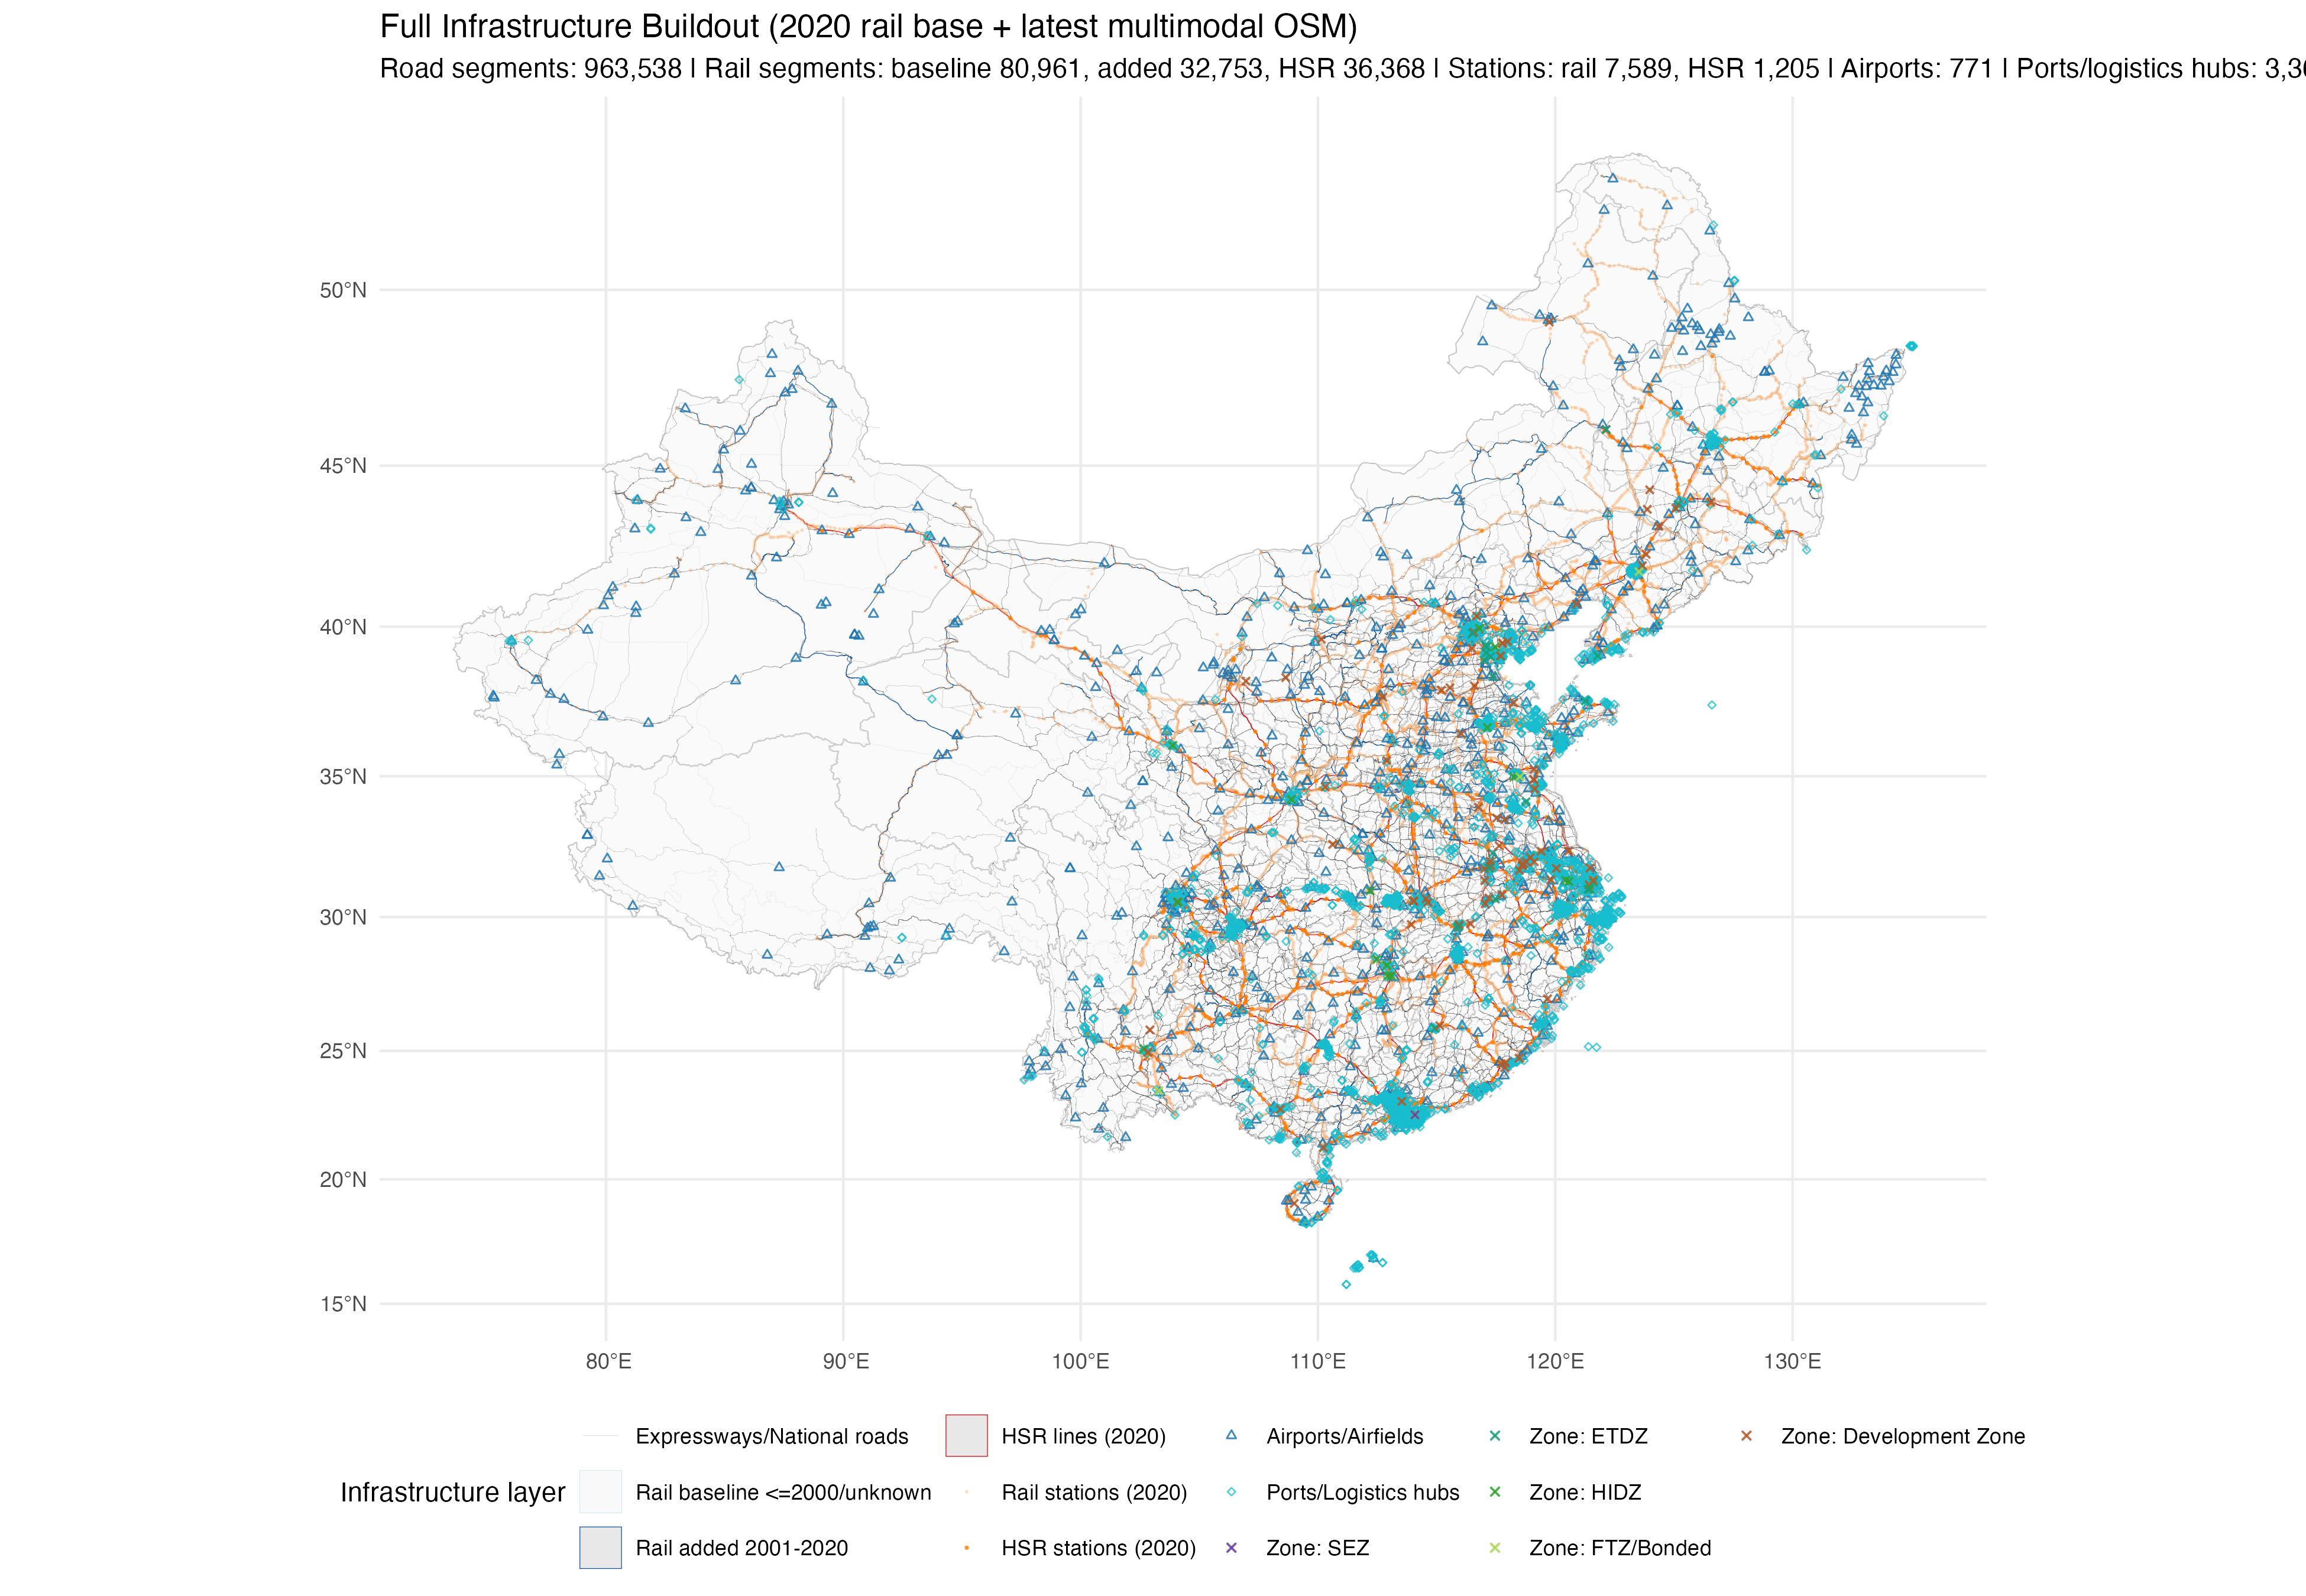
\includegraphics[width=0.97\linewidth,height=0.82\textheight,keepaspectratio]{outputs/figures/map_16_full_infrastructure_buildout.png}
\end{frame}

\begin{frame}{Rail and HSR Expansion Chronology}
\centering
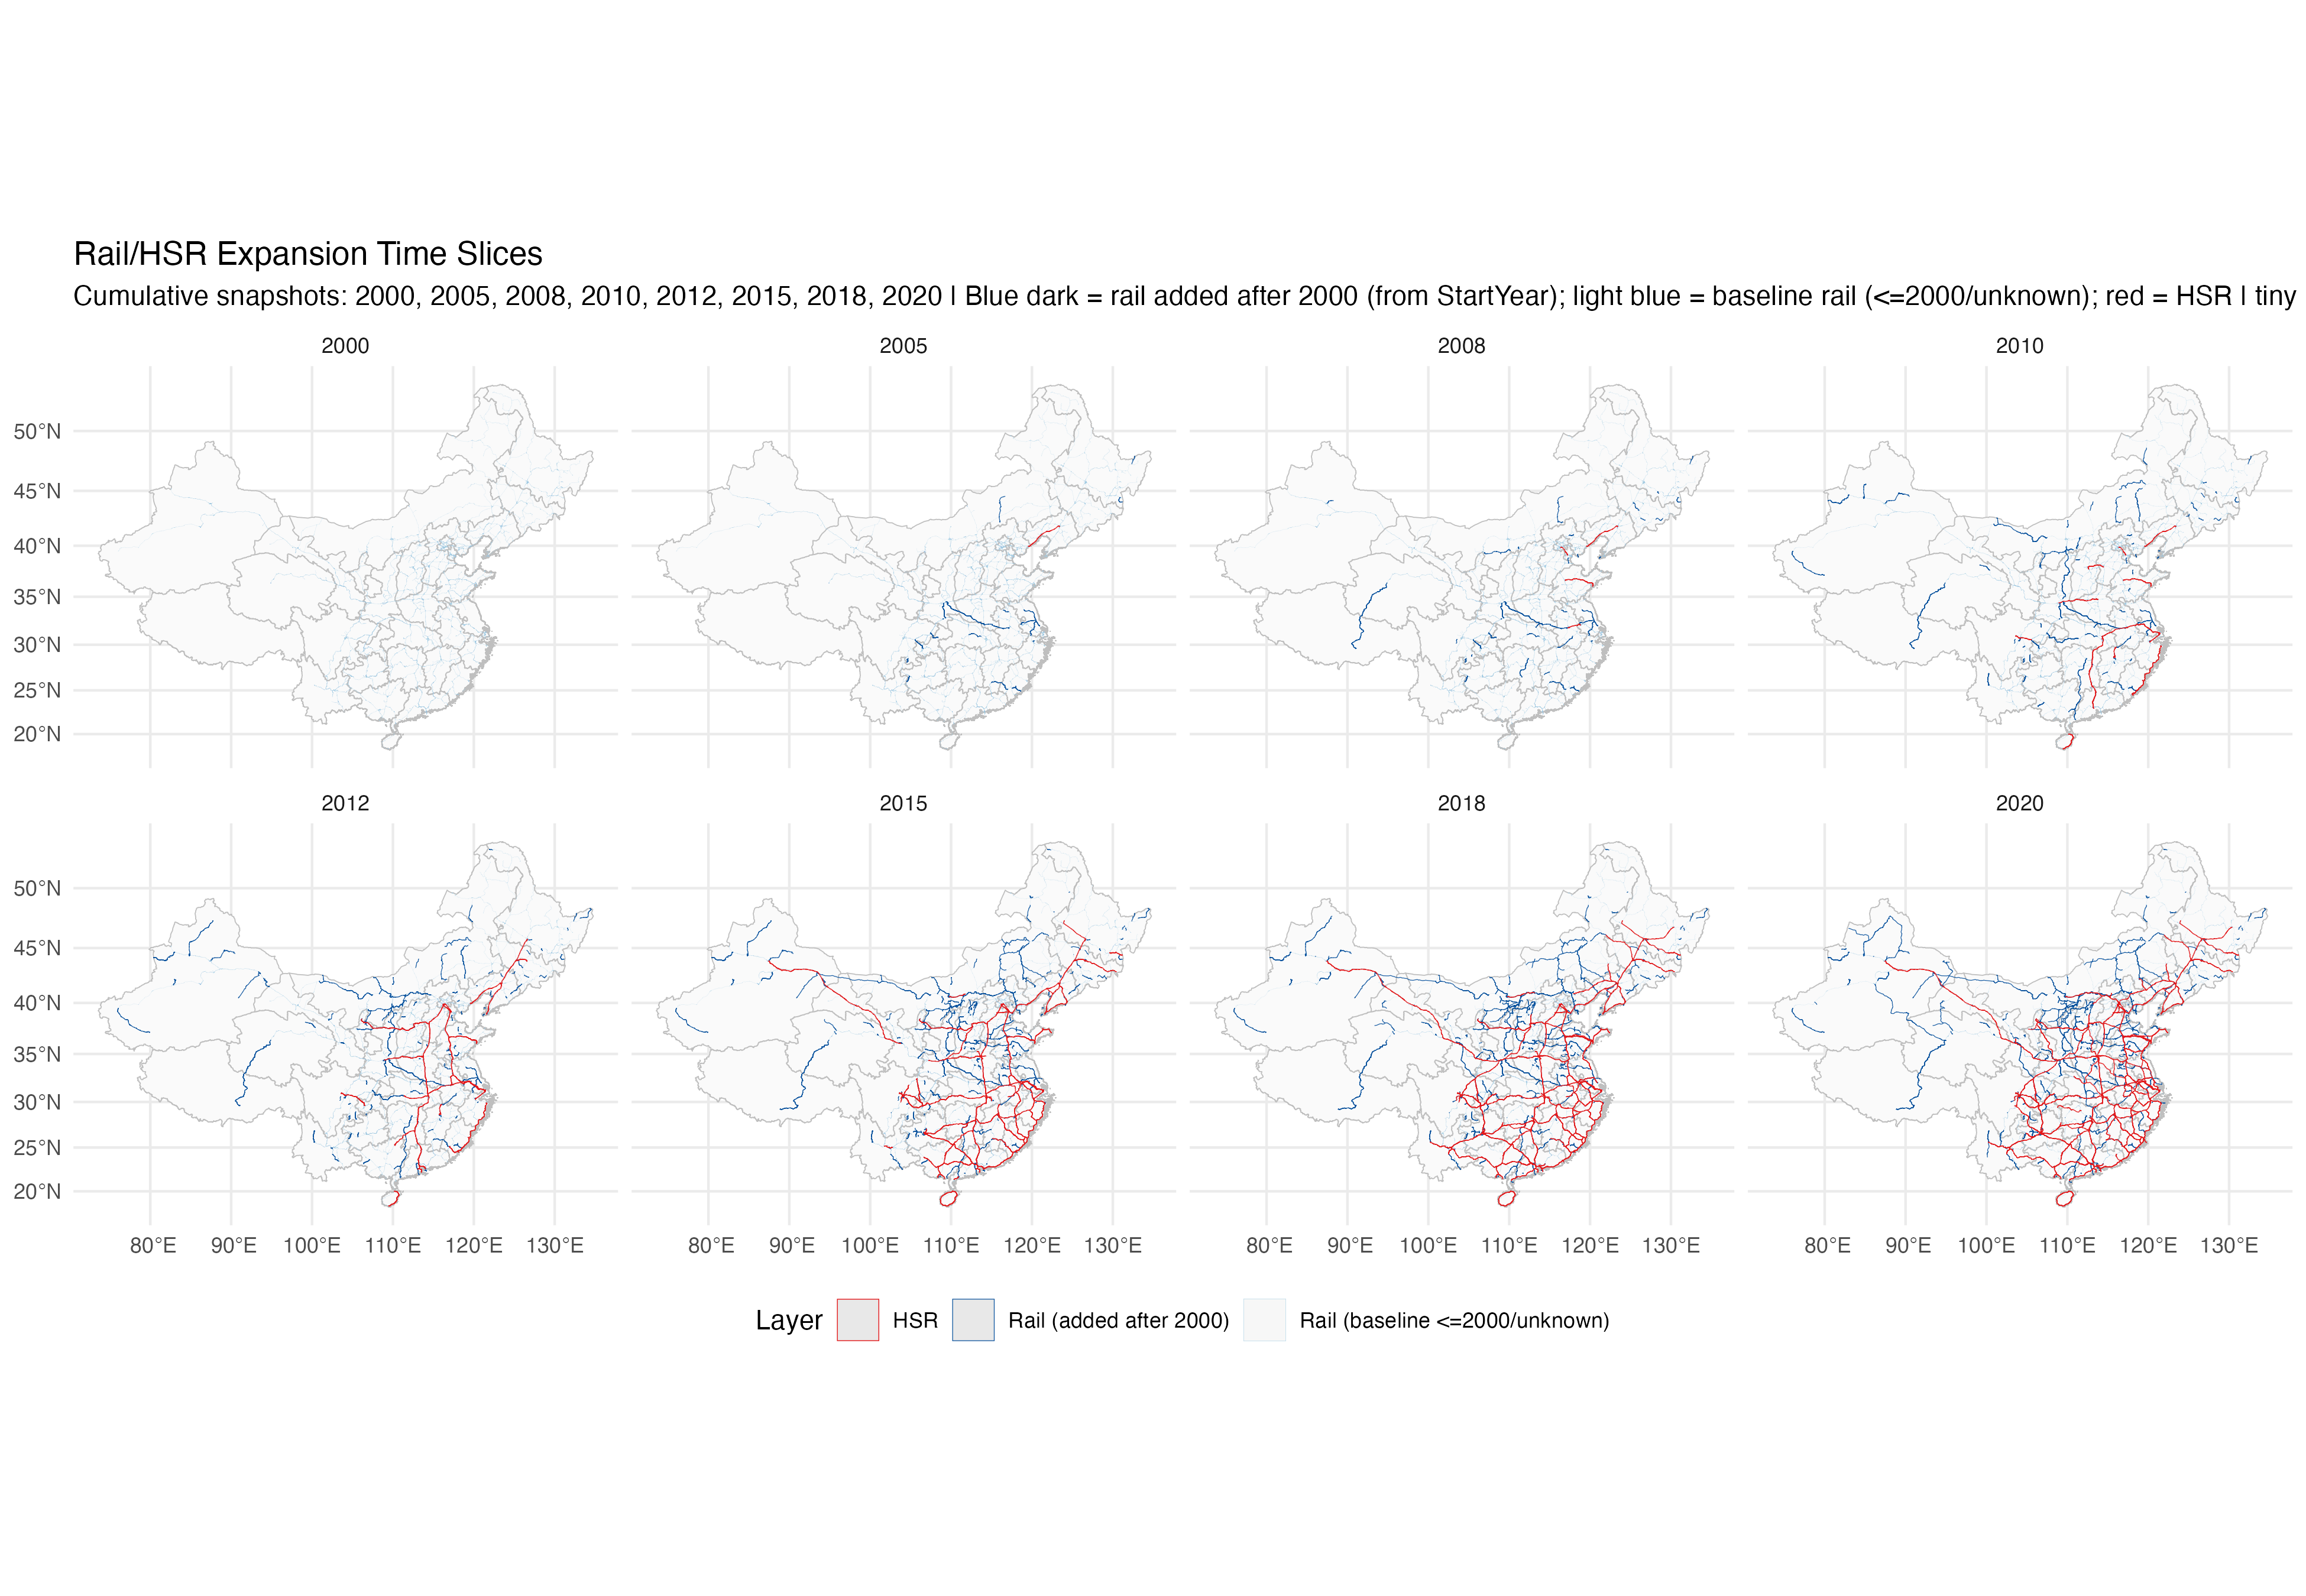
\includegraphics[width=0.97\linewidth,height=0.82\textheight,keepaspectratio]{outputs/figures/map_01_rail_hsr_timeslices.png}
\end{frame}

\begin{frame}{Aggregate Network Dynamics Over Time}
\small
\begin{columns}[T,onlytextwidth]
\column{0.62\linewidth}
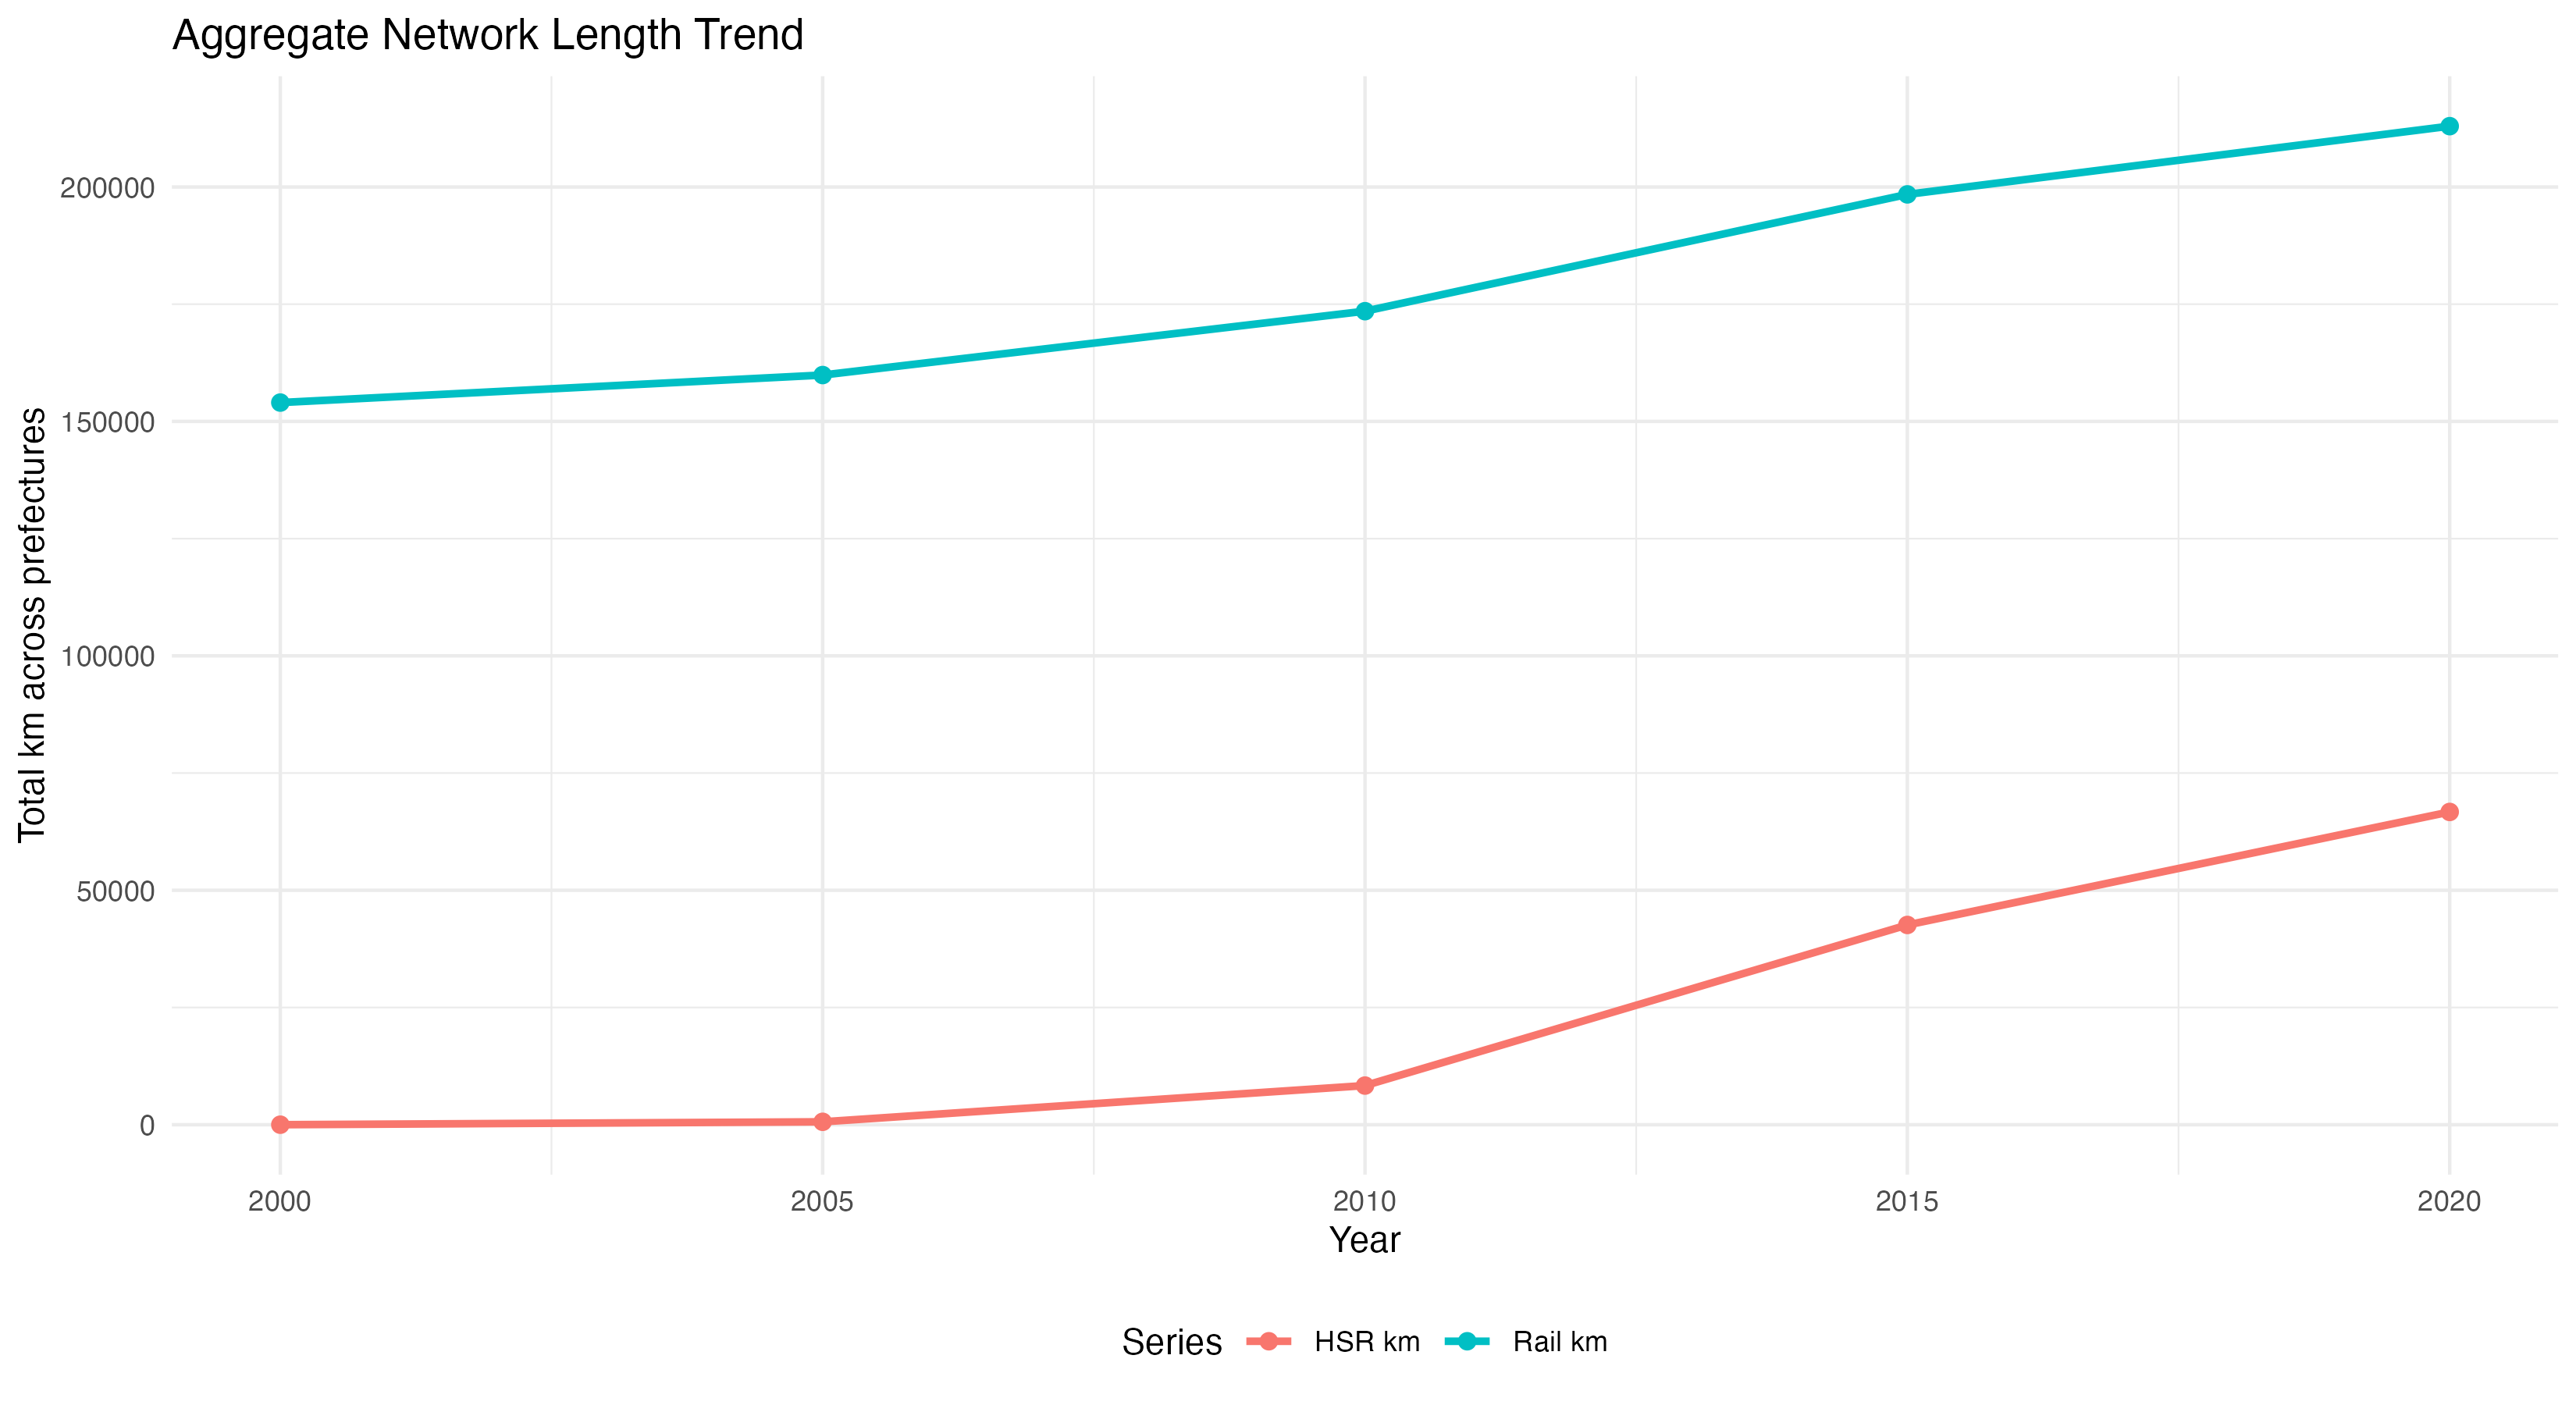
\includegraphics[width=\linewidth,height=0.76\textheight,keepaspectratio]{outputs/figures/fig_19_network_length_trend.png}
\column{0.35\linewidth}
\justifying
\textbf{Readout:}
\begin{itemize}
  \item Strong cumulative network buildout across the panel years.
  \item HSR stock emerges later and then rises quickly, while regular rail remains the dominant base.
  \item This confirms that spatial outcomes are observed under substantial connectivity regime change, not static infrastructure.
\end{itemize}
\end{columns}
\end{frame}

\begin{frame}{Integrated Synergy Hotspots}
\centering
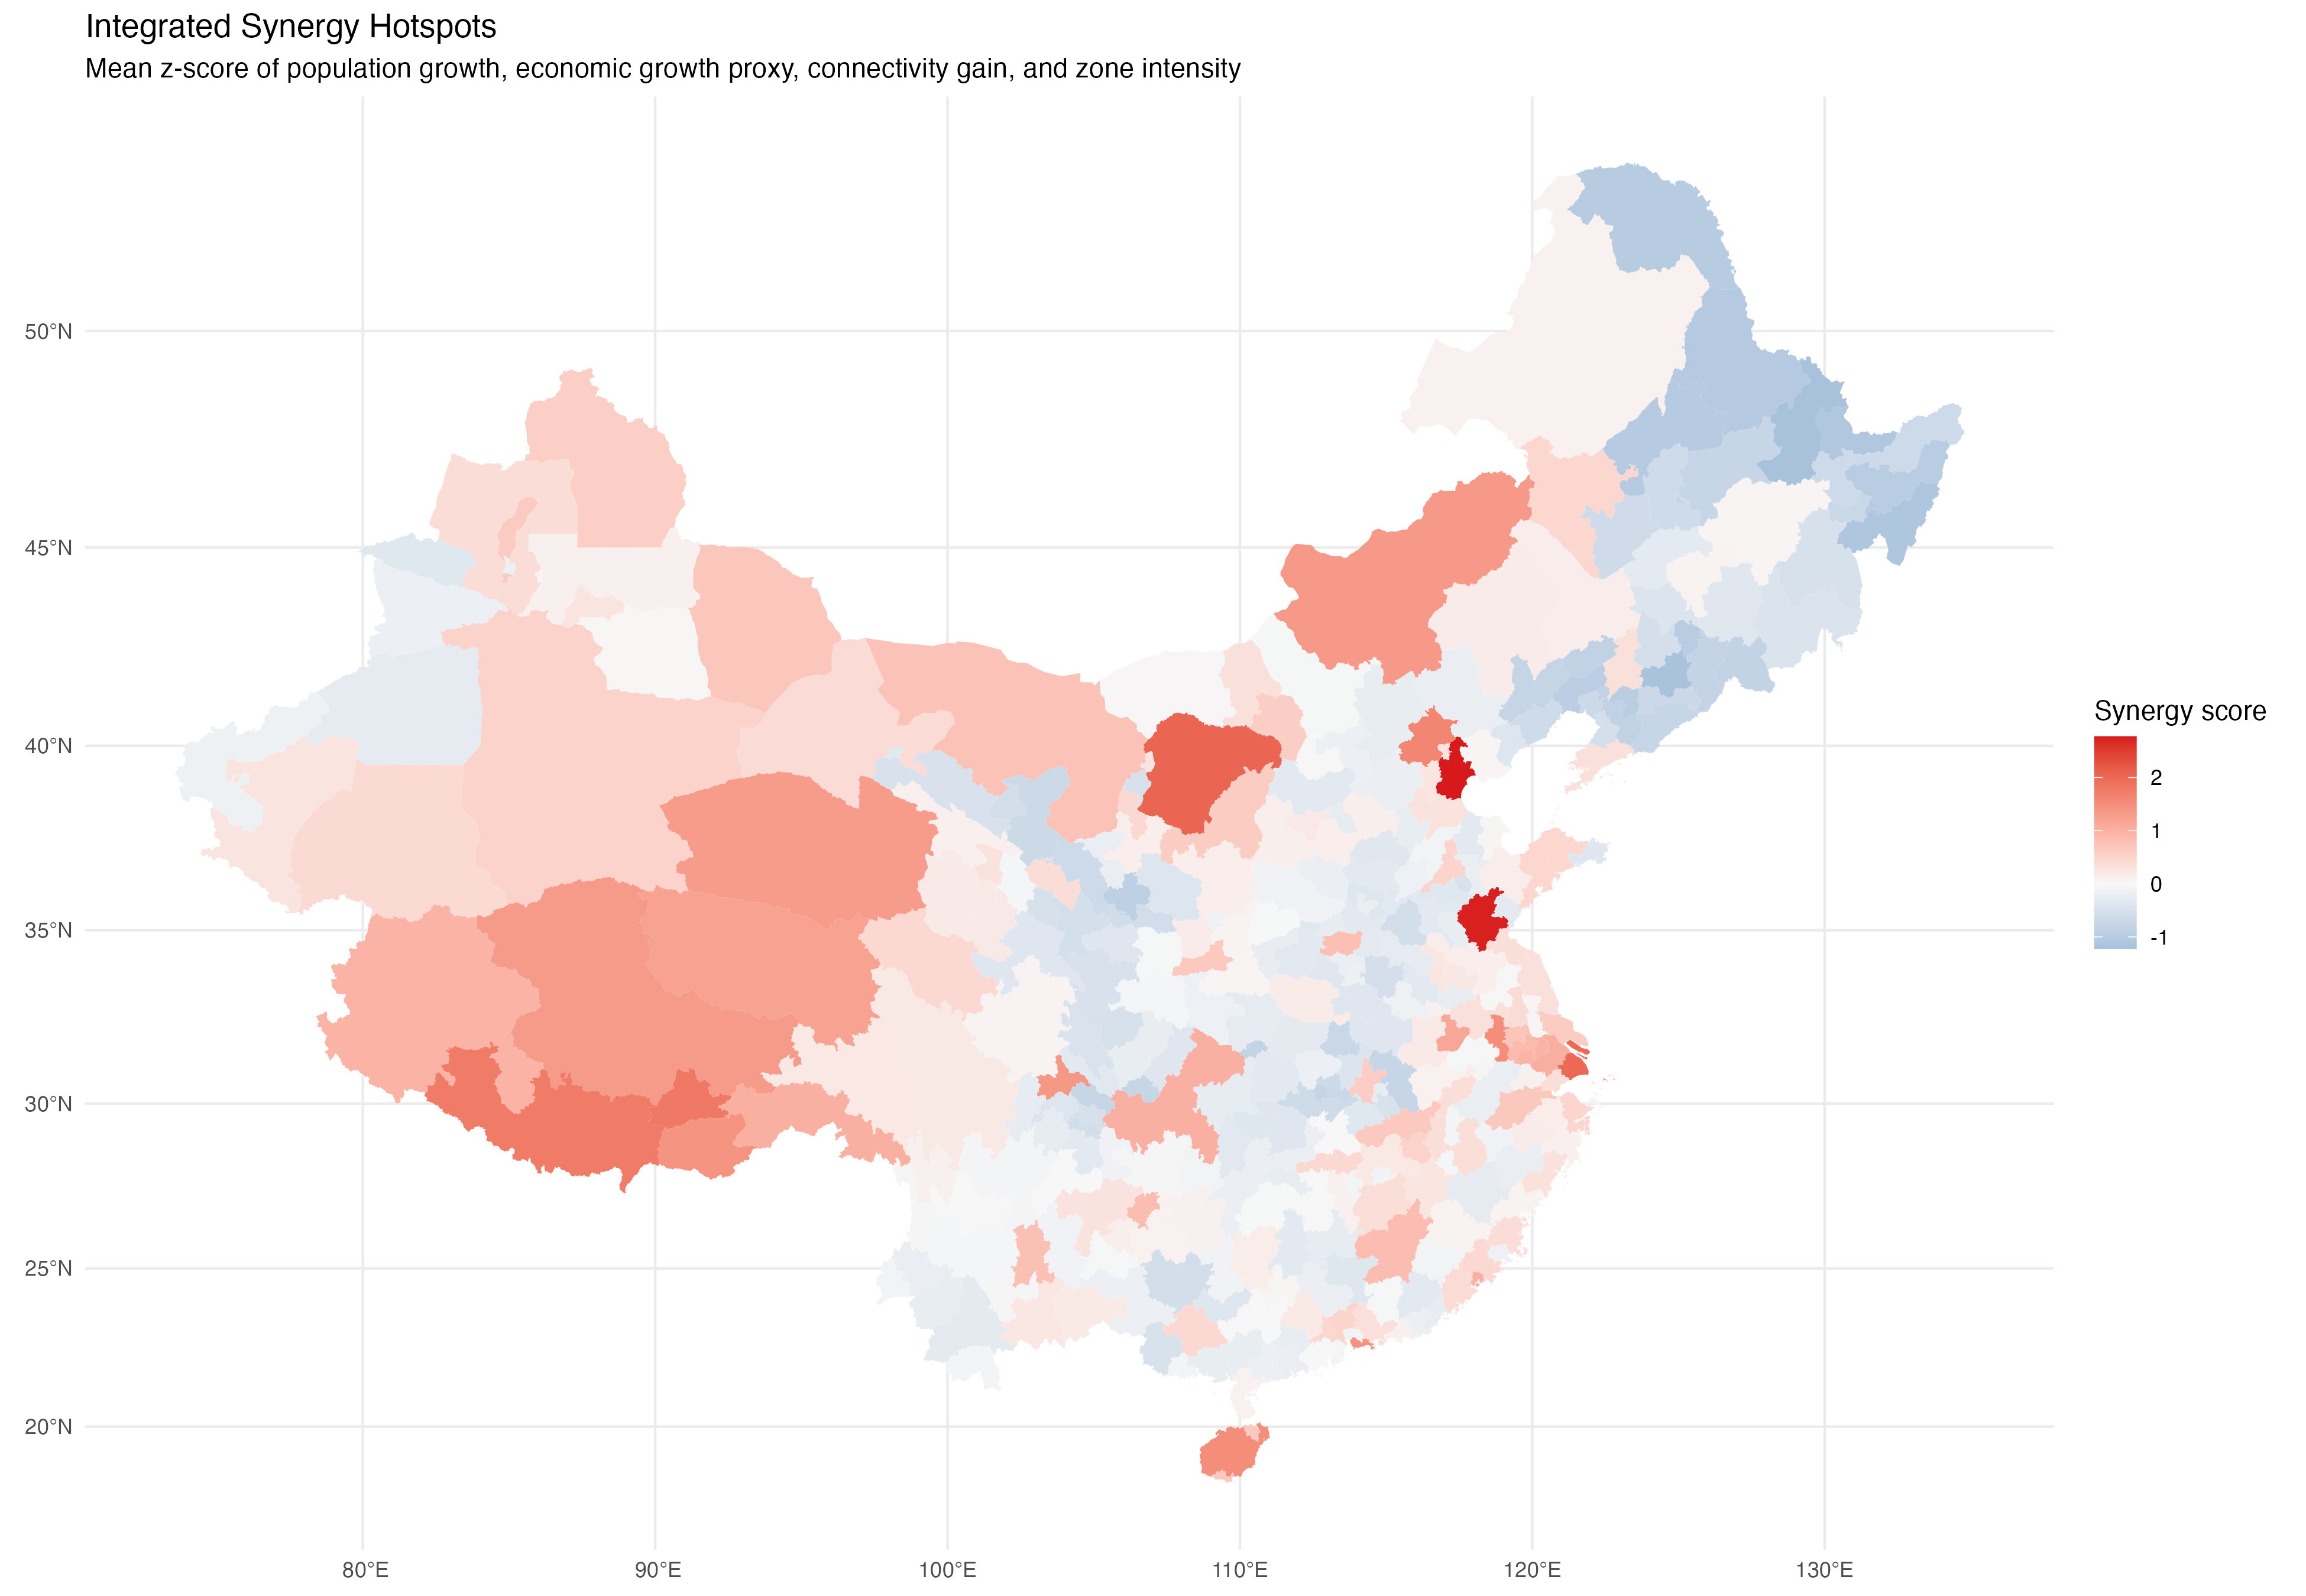
\includegraphics[width=0.97\linewidth,height=0.82\textheight,keepaspectratio]{outputs/figures/map_17_synergy_hotspots.png}
\end{frame}

\begin{frame}{Population-Growth Geography}
\centering
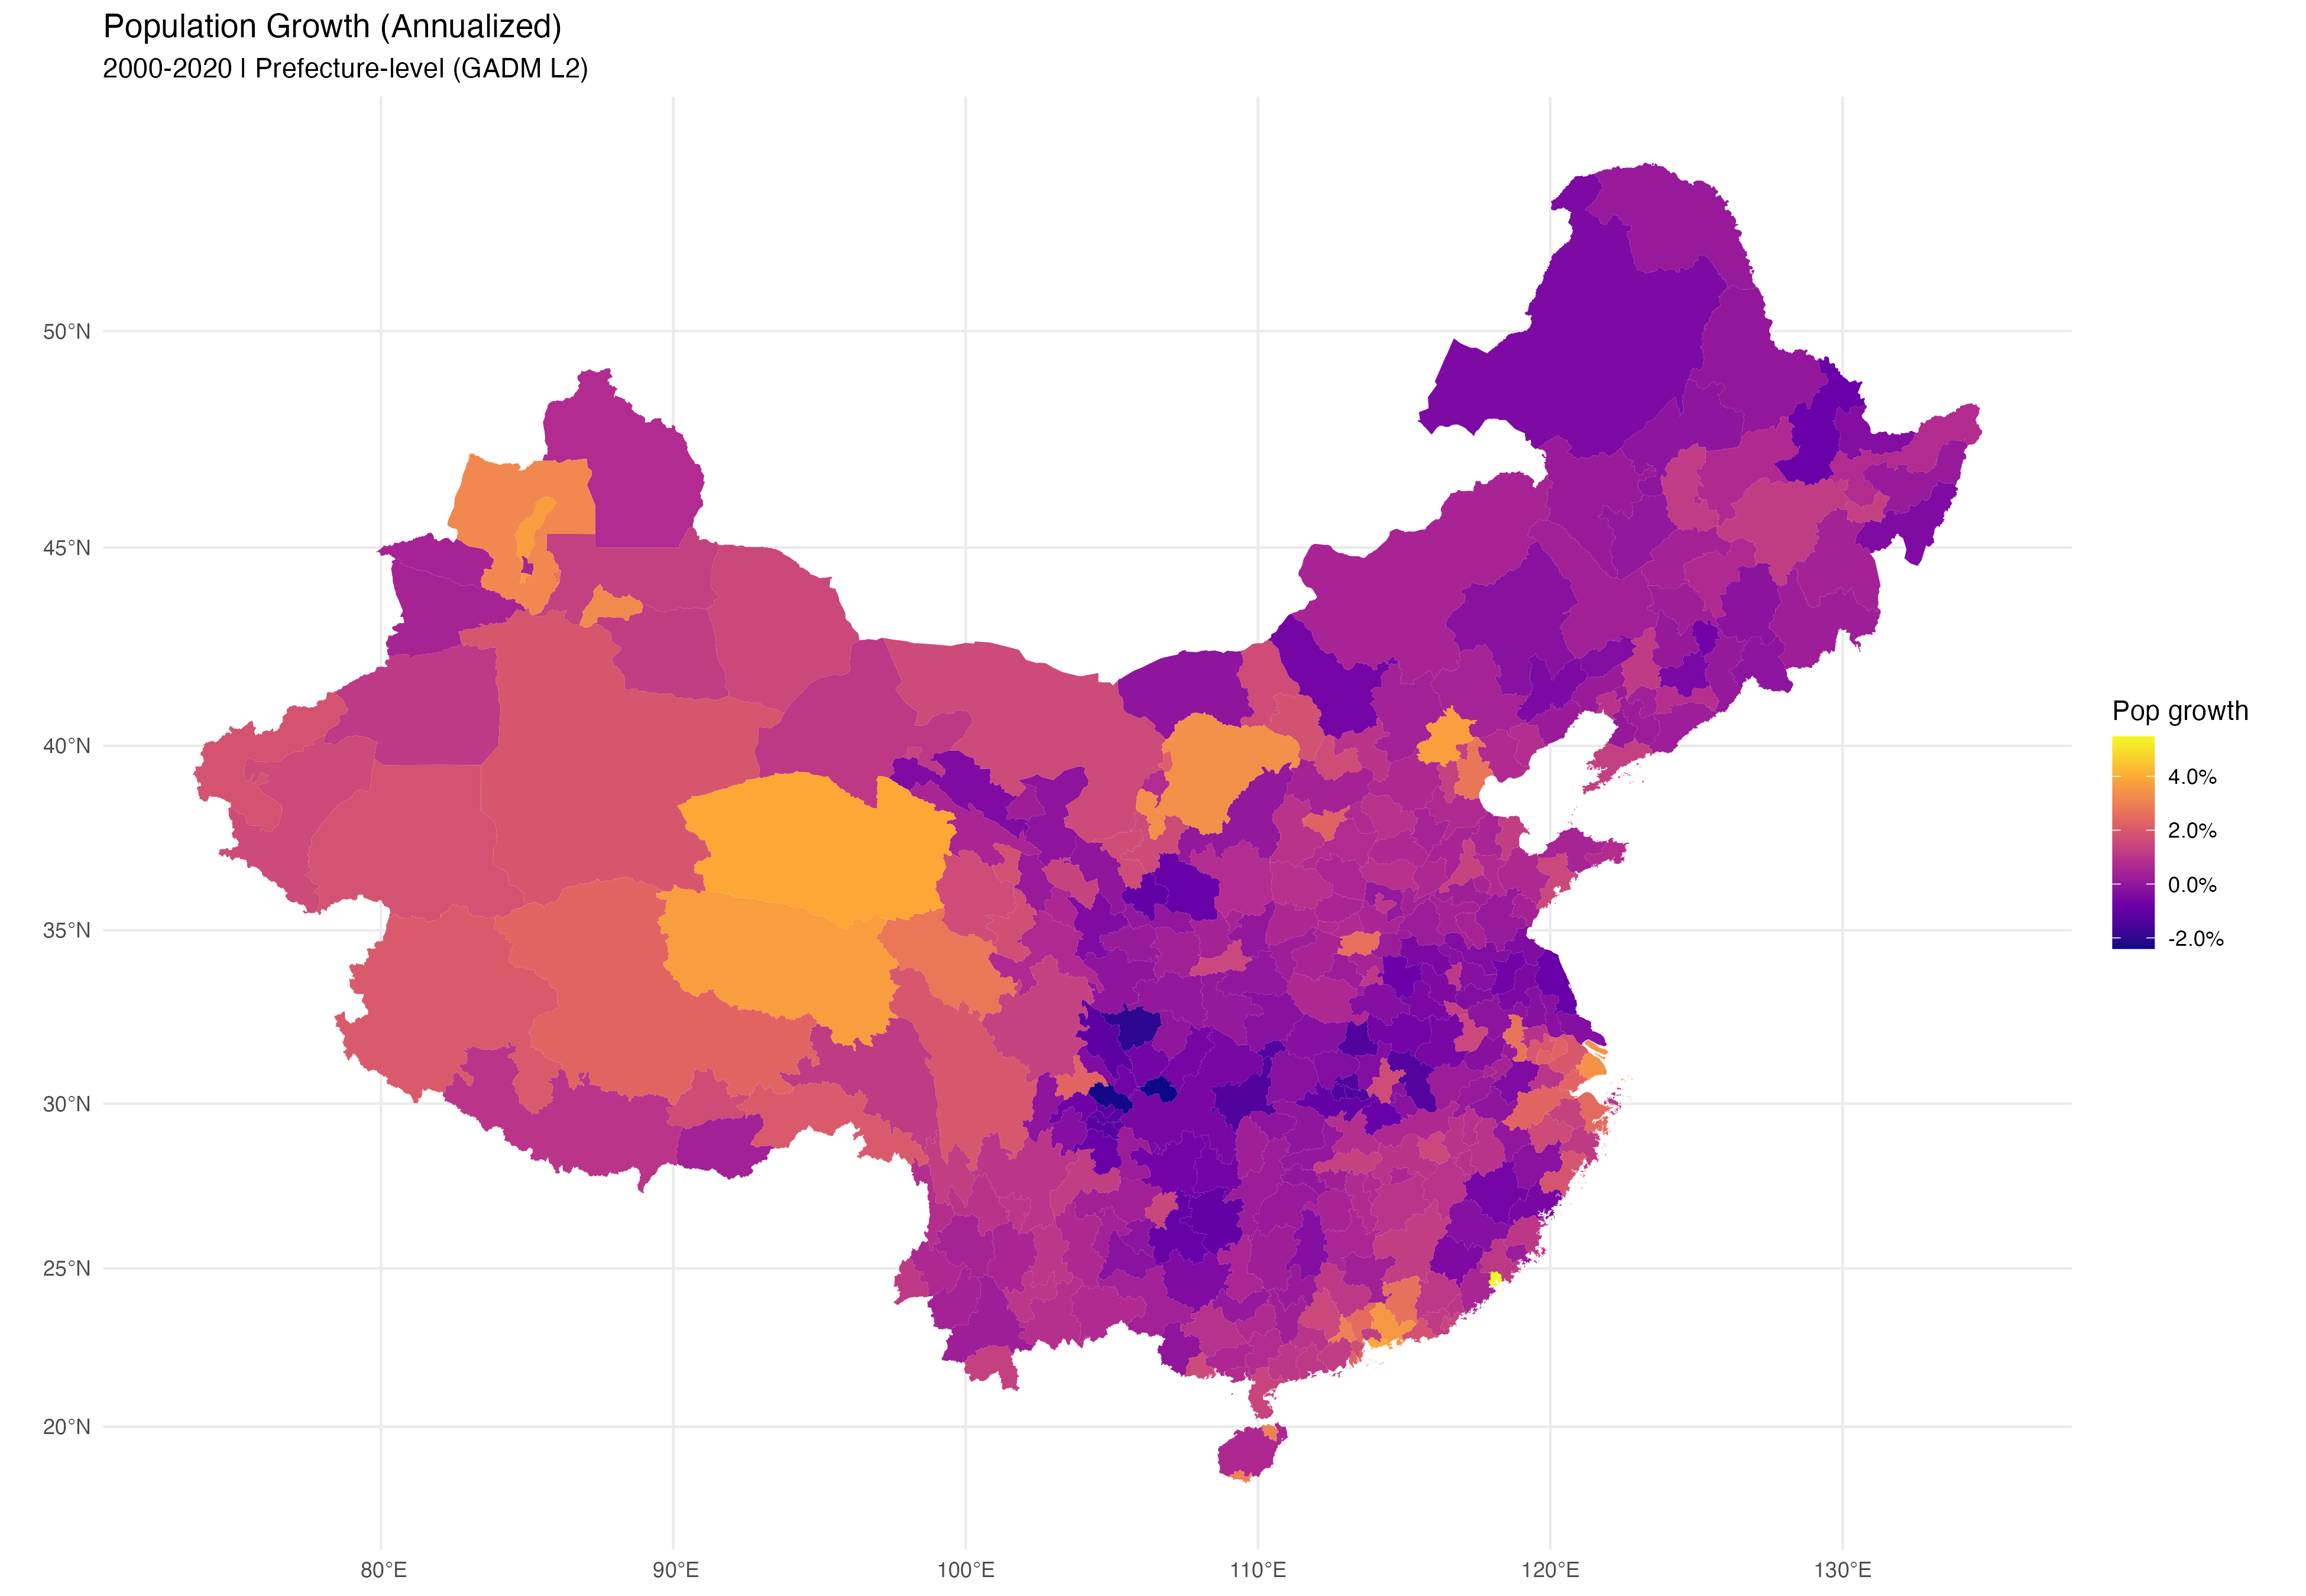
\includegraphics[width=0.97\linewidth,height=0.82\textheight,keepaspectratio]{outputs/figures/map_03_population_growth.png}
\end{frame}

\begin{frame}{Economic-Growth-Proxy Geography}
\centering
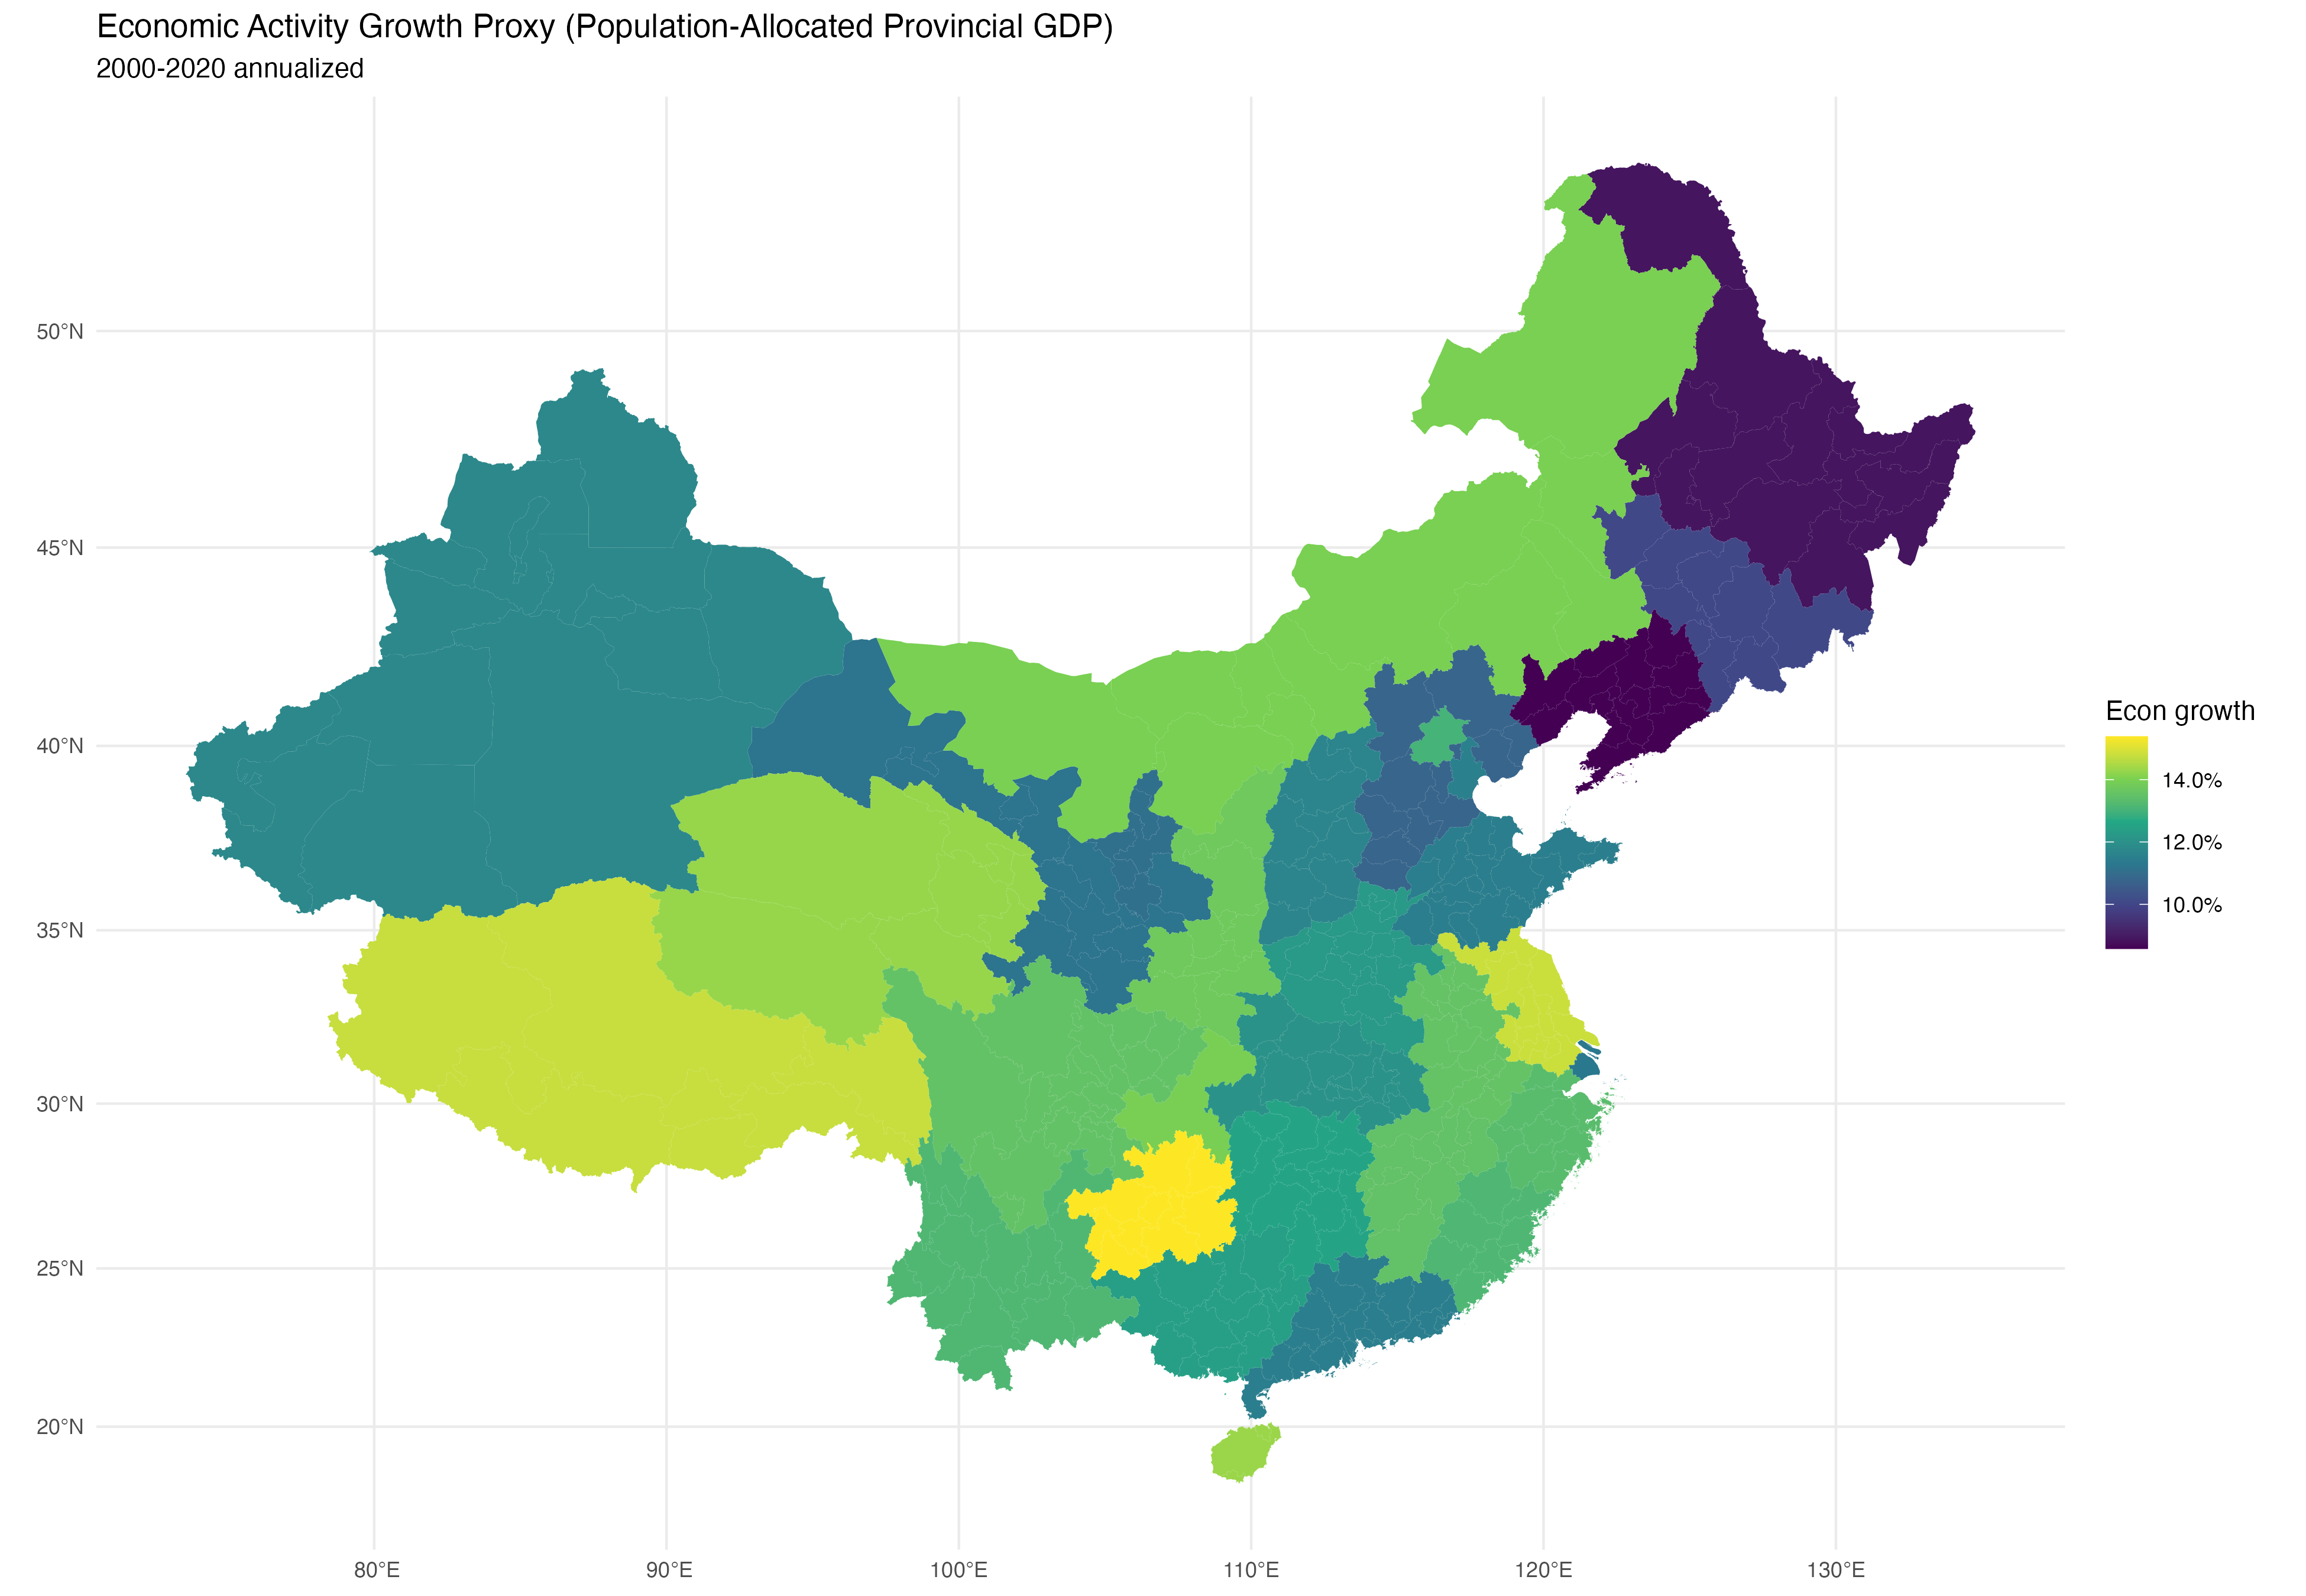
\includegraphics[width=0.97\linewidth,height=0.82\textheight,keepaspectratio]{outputs/figures/map_04_economic_growth_proxy.png}
\end{frame}

\begin{frame}{Trajectory Typology Map}
\centering
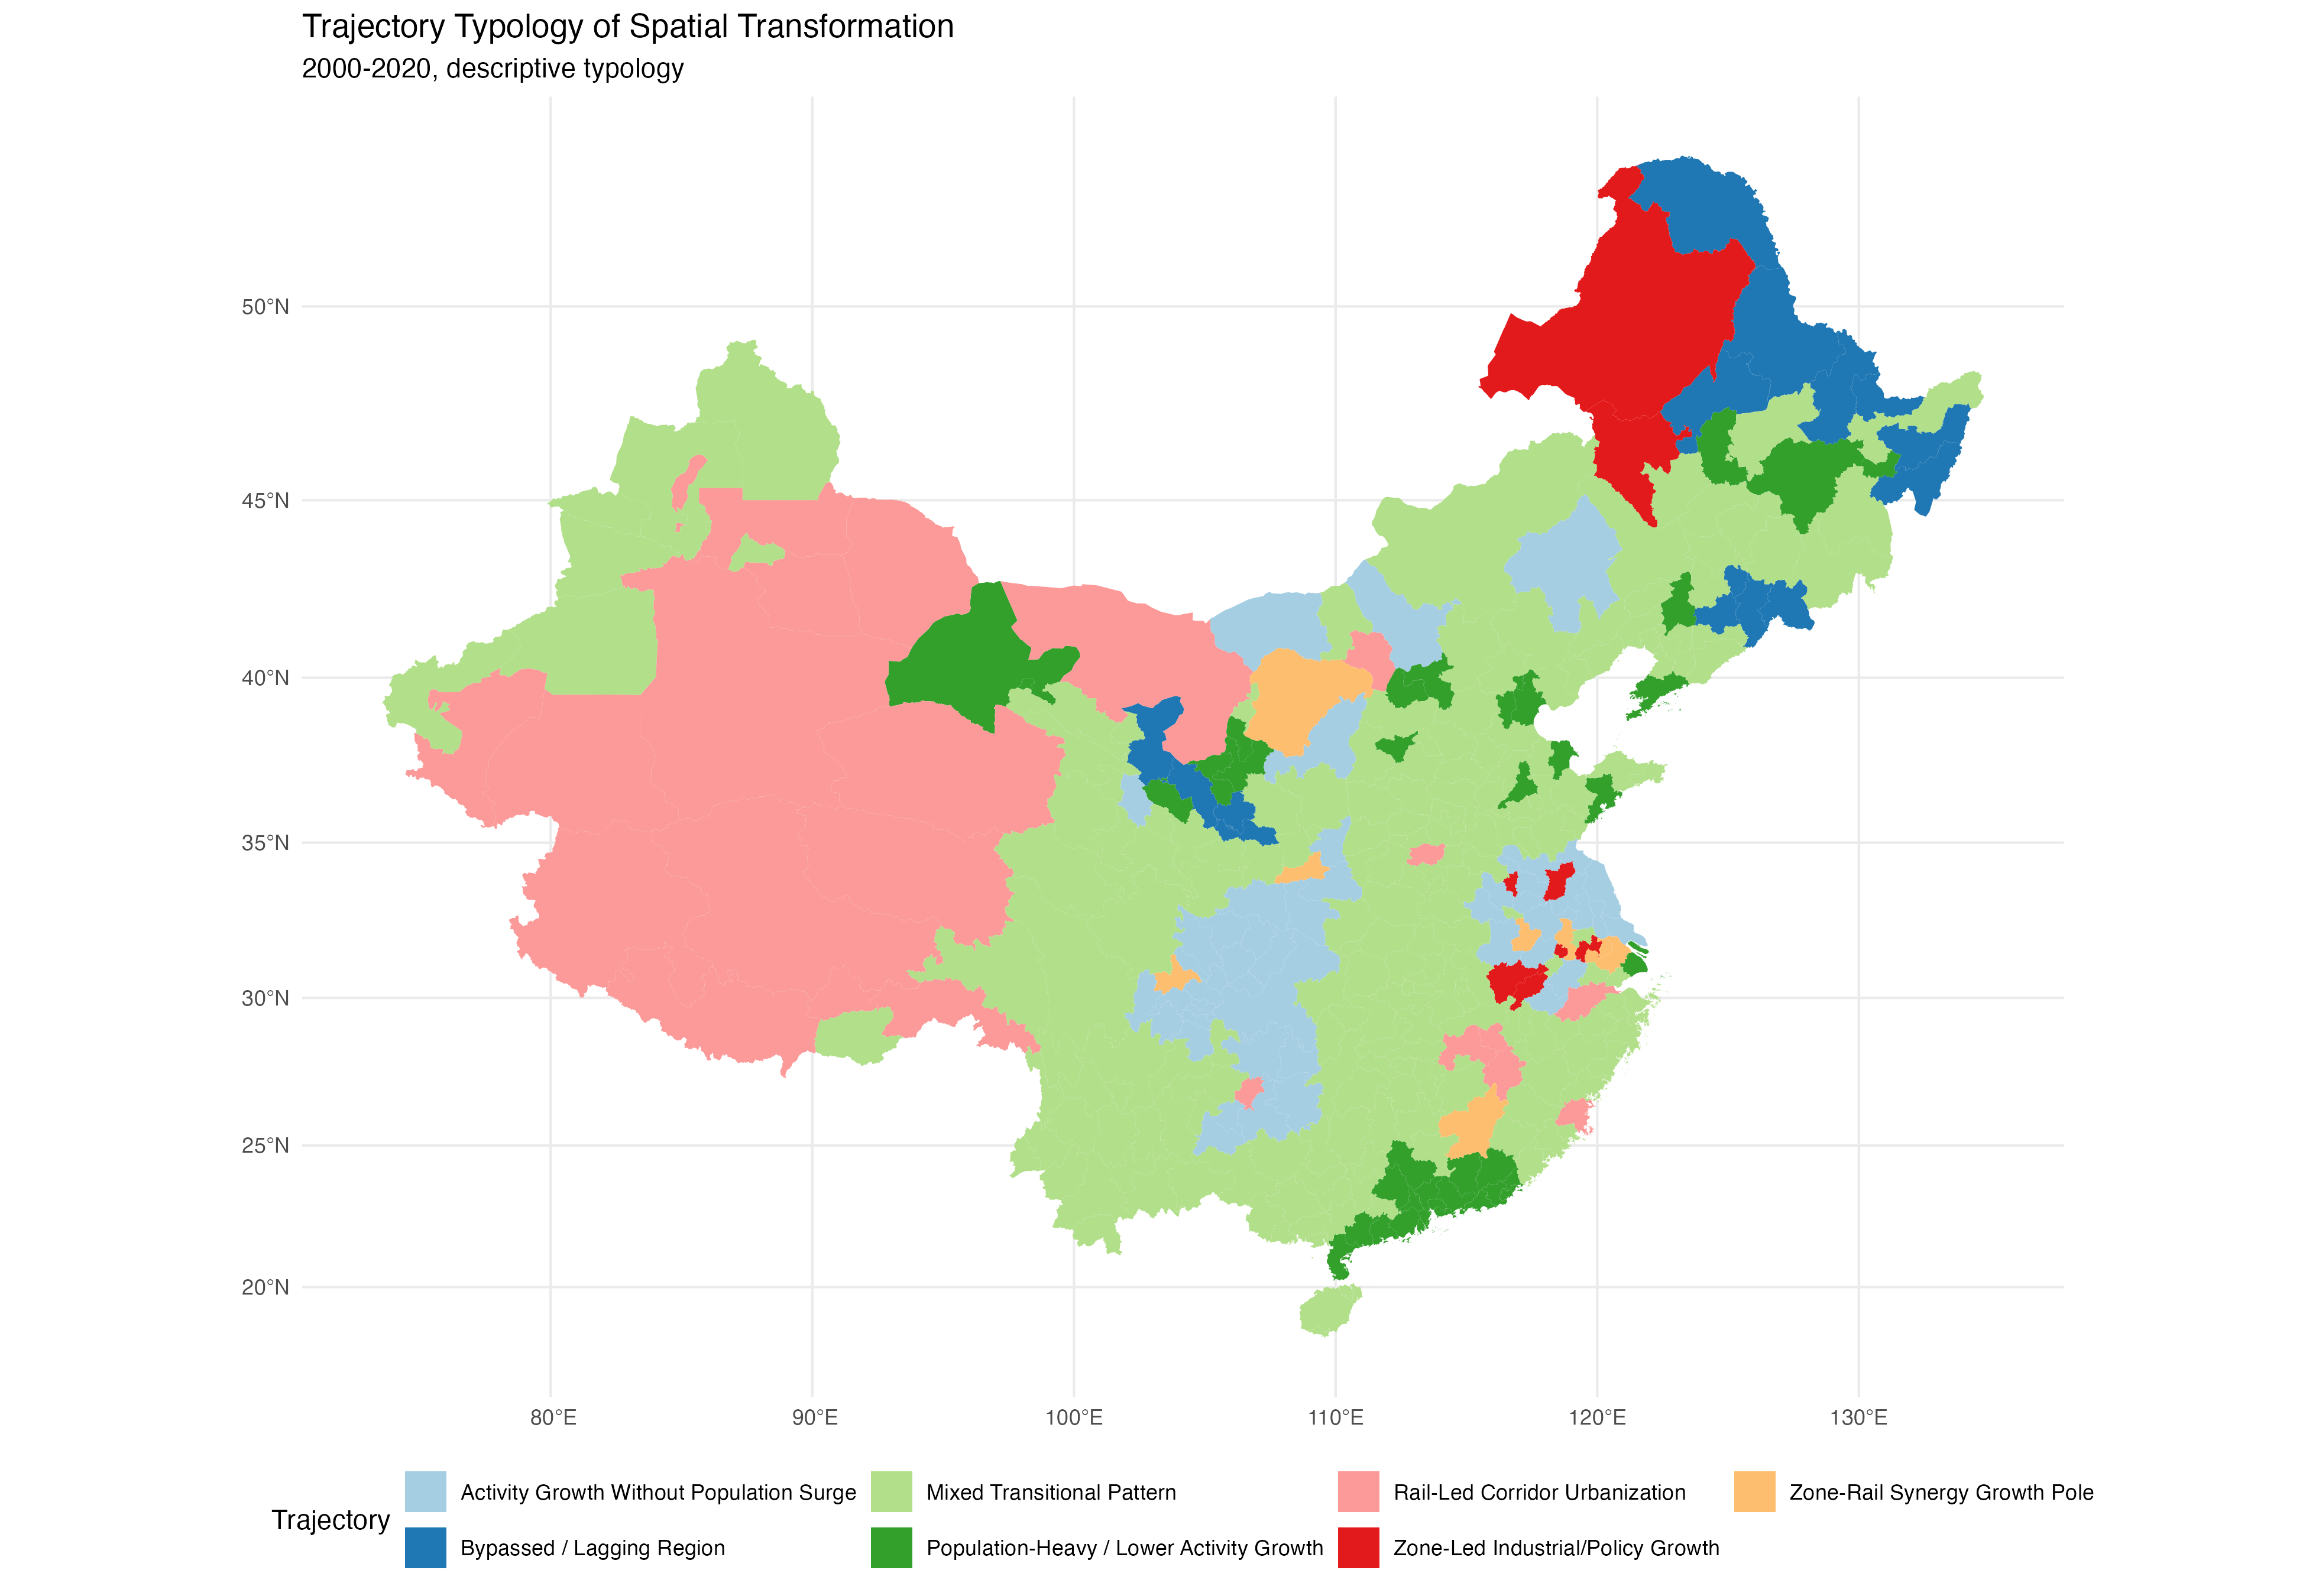
\includegraphics[width=0.97\linewidth,height=0.82\textheight,keepaspectratio]{outputs/figures/map_07_typology_prefecture.png}
\end{frame}

\begin{frame}{Typology Composition and Mean Profiles}
\small
\begin{columns}[T,onlytextwidth]
\column{0.54\linewidth}
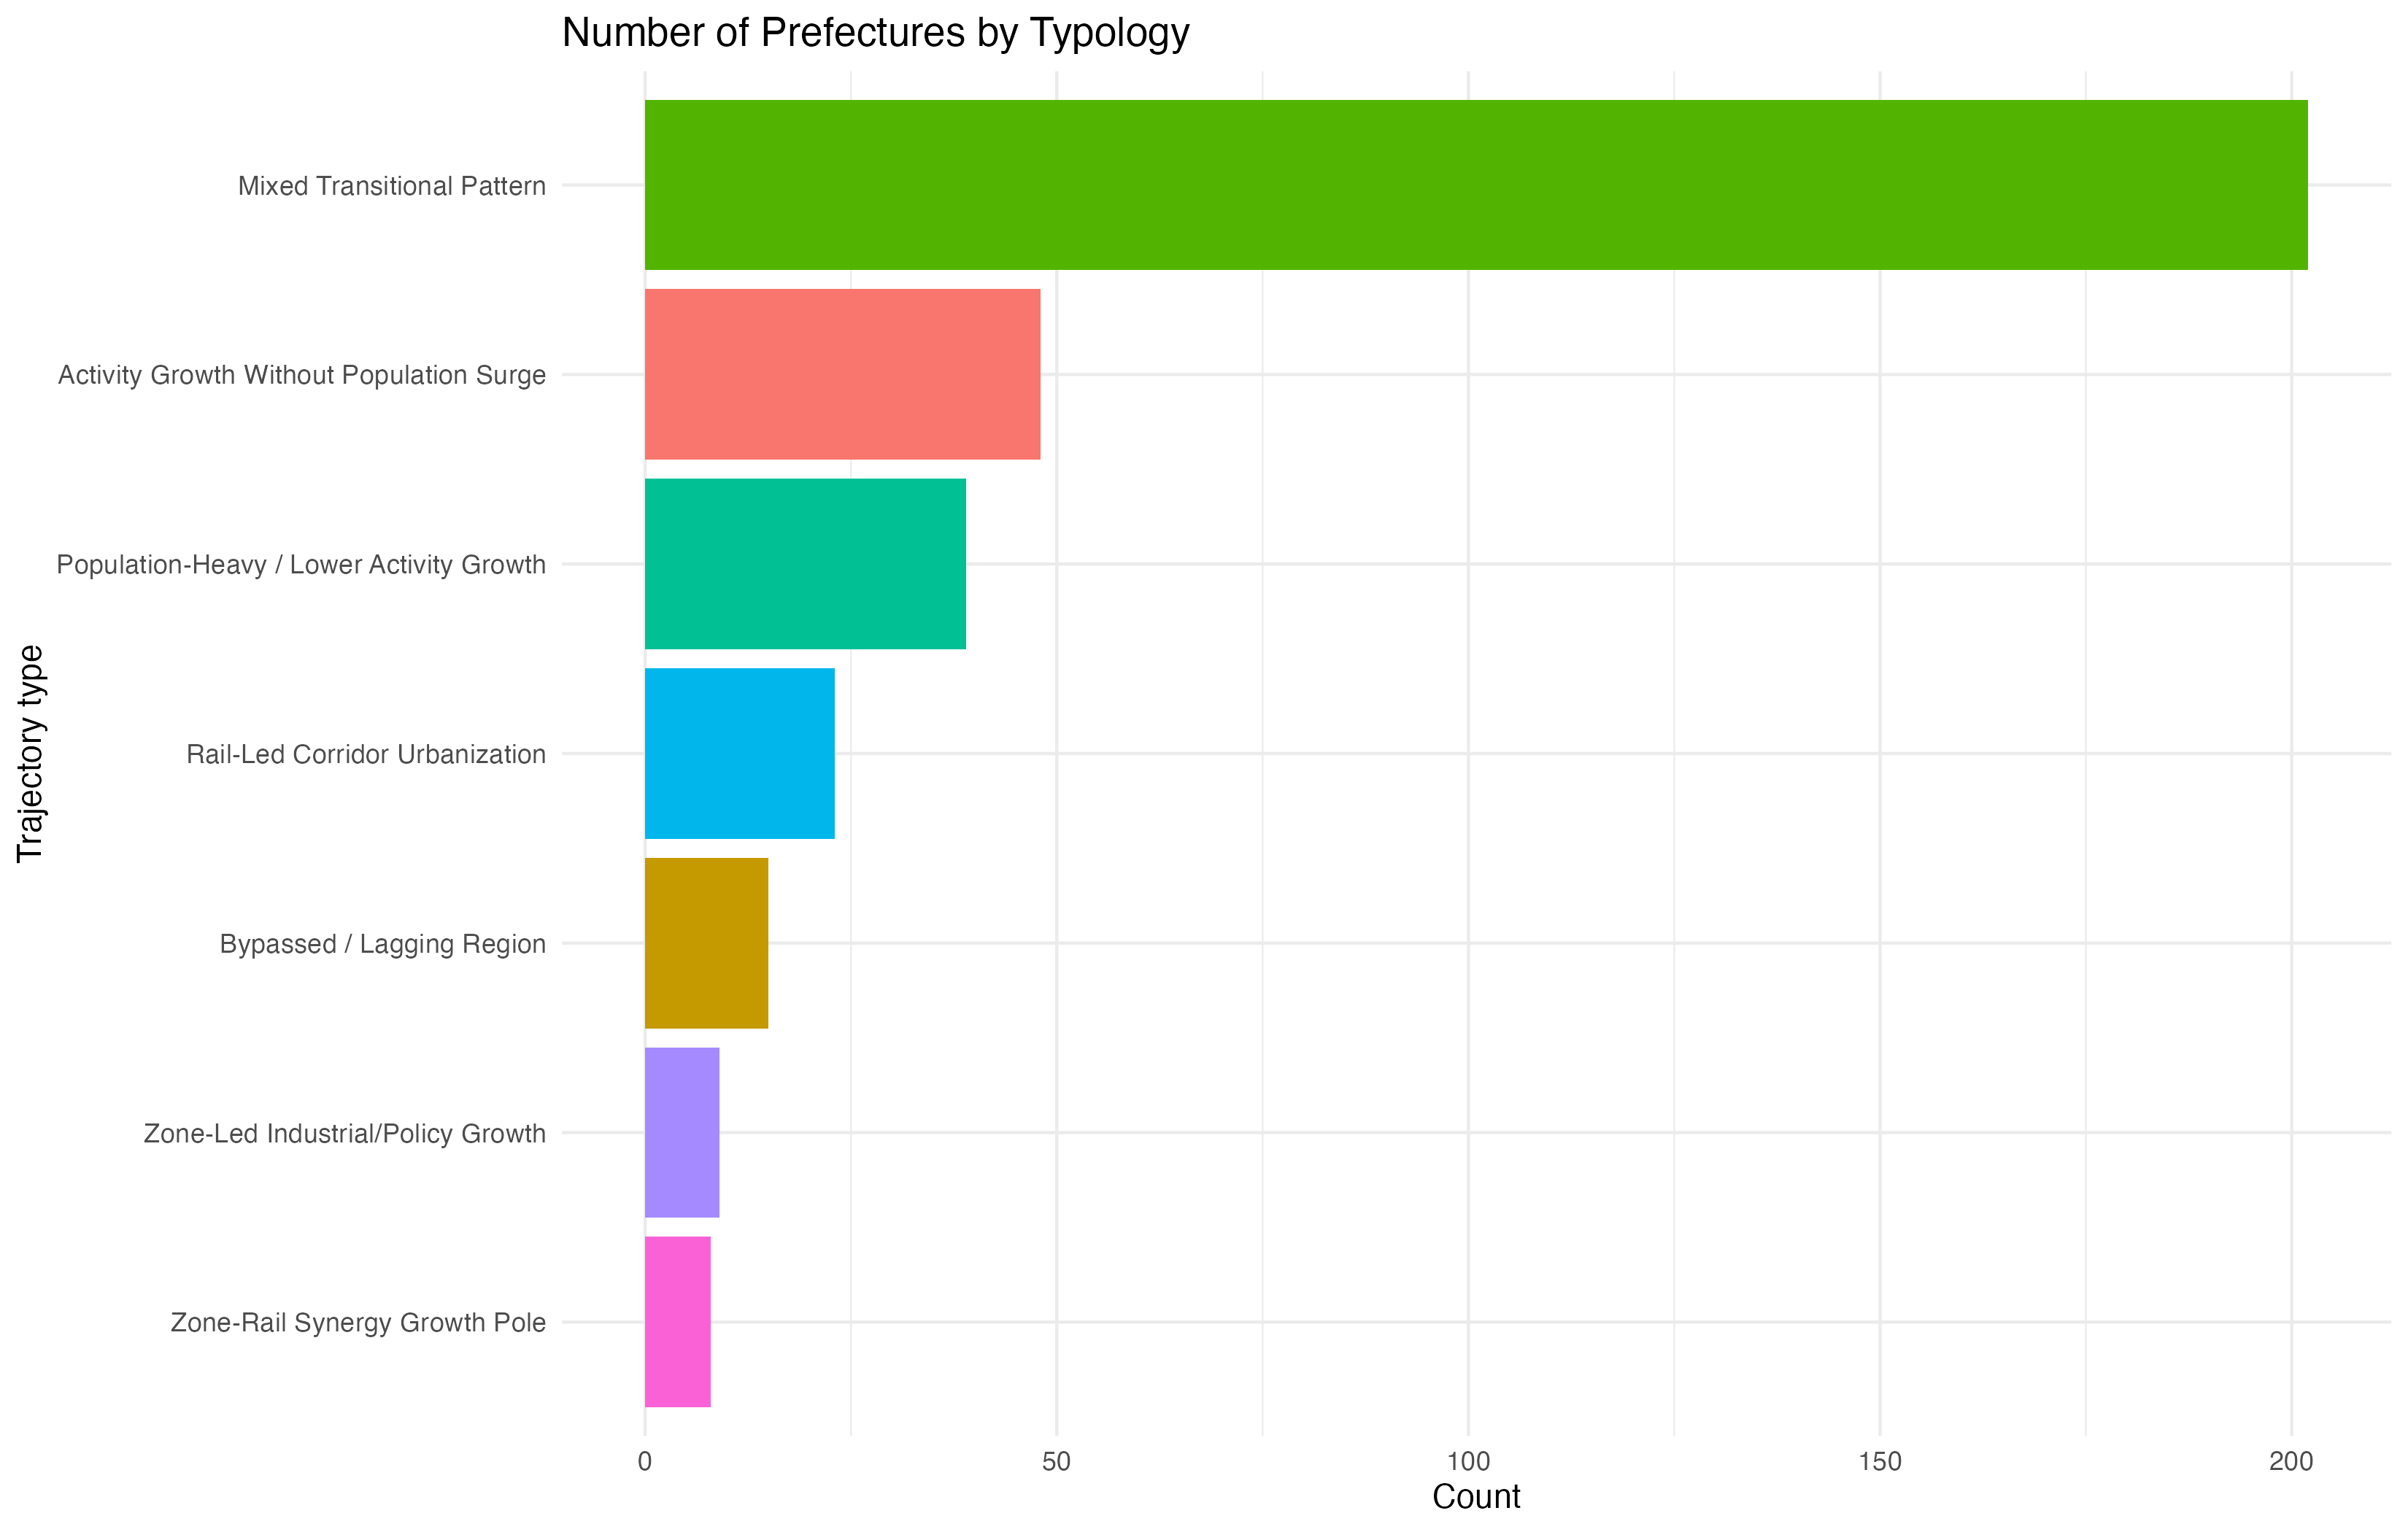
\includegraphics[width=\linewidth,height=0.76\textheight,keepaspectratio]{outputs/figures/fig_15_typology_counts.png}
\column{0.44\linewidth}
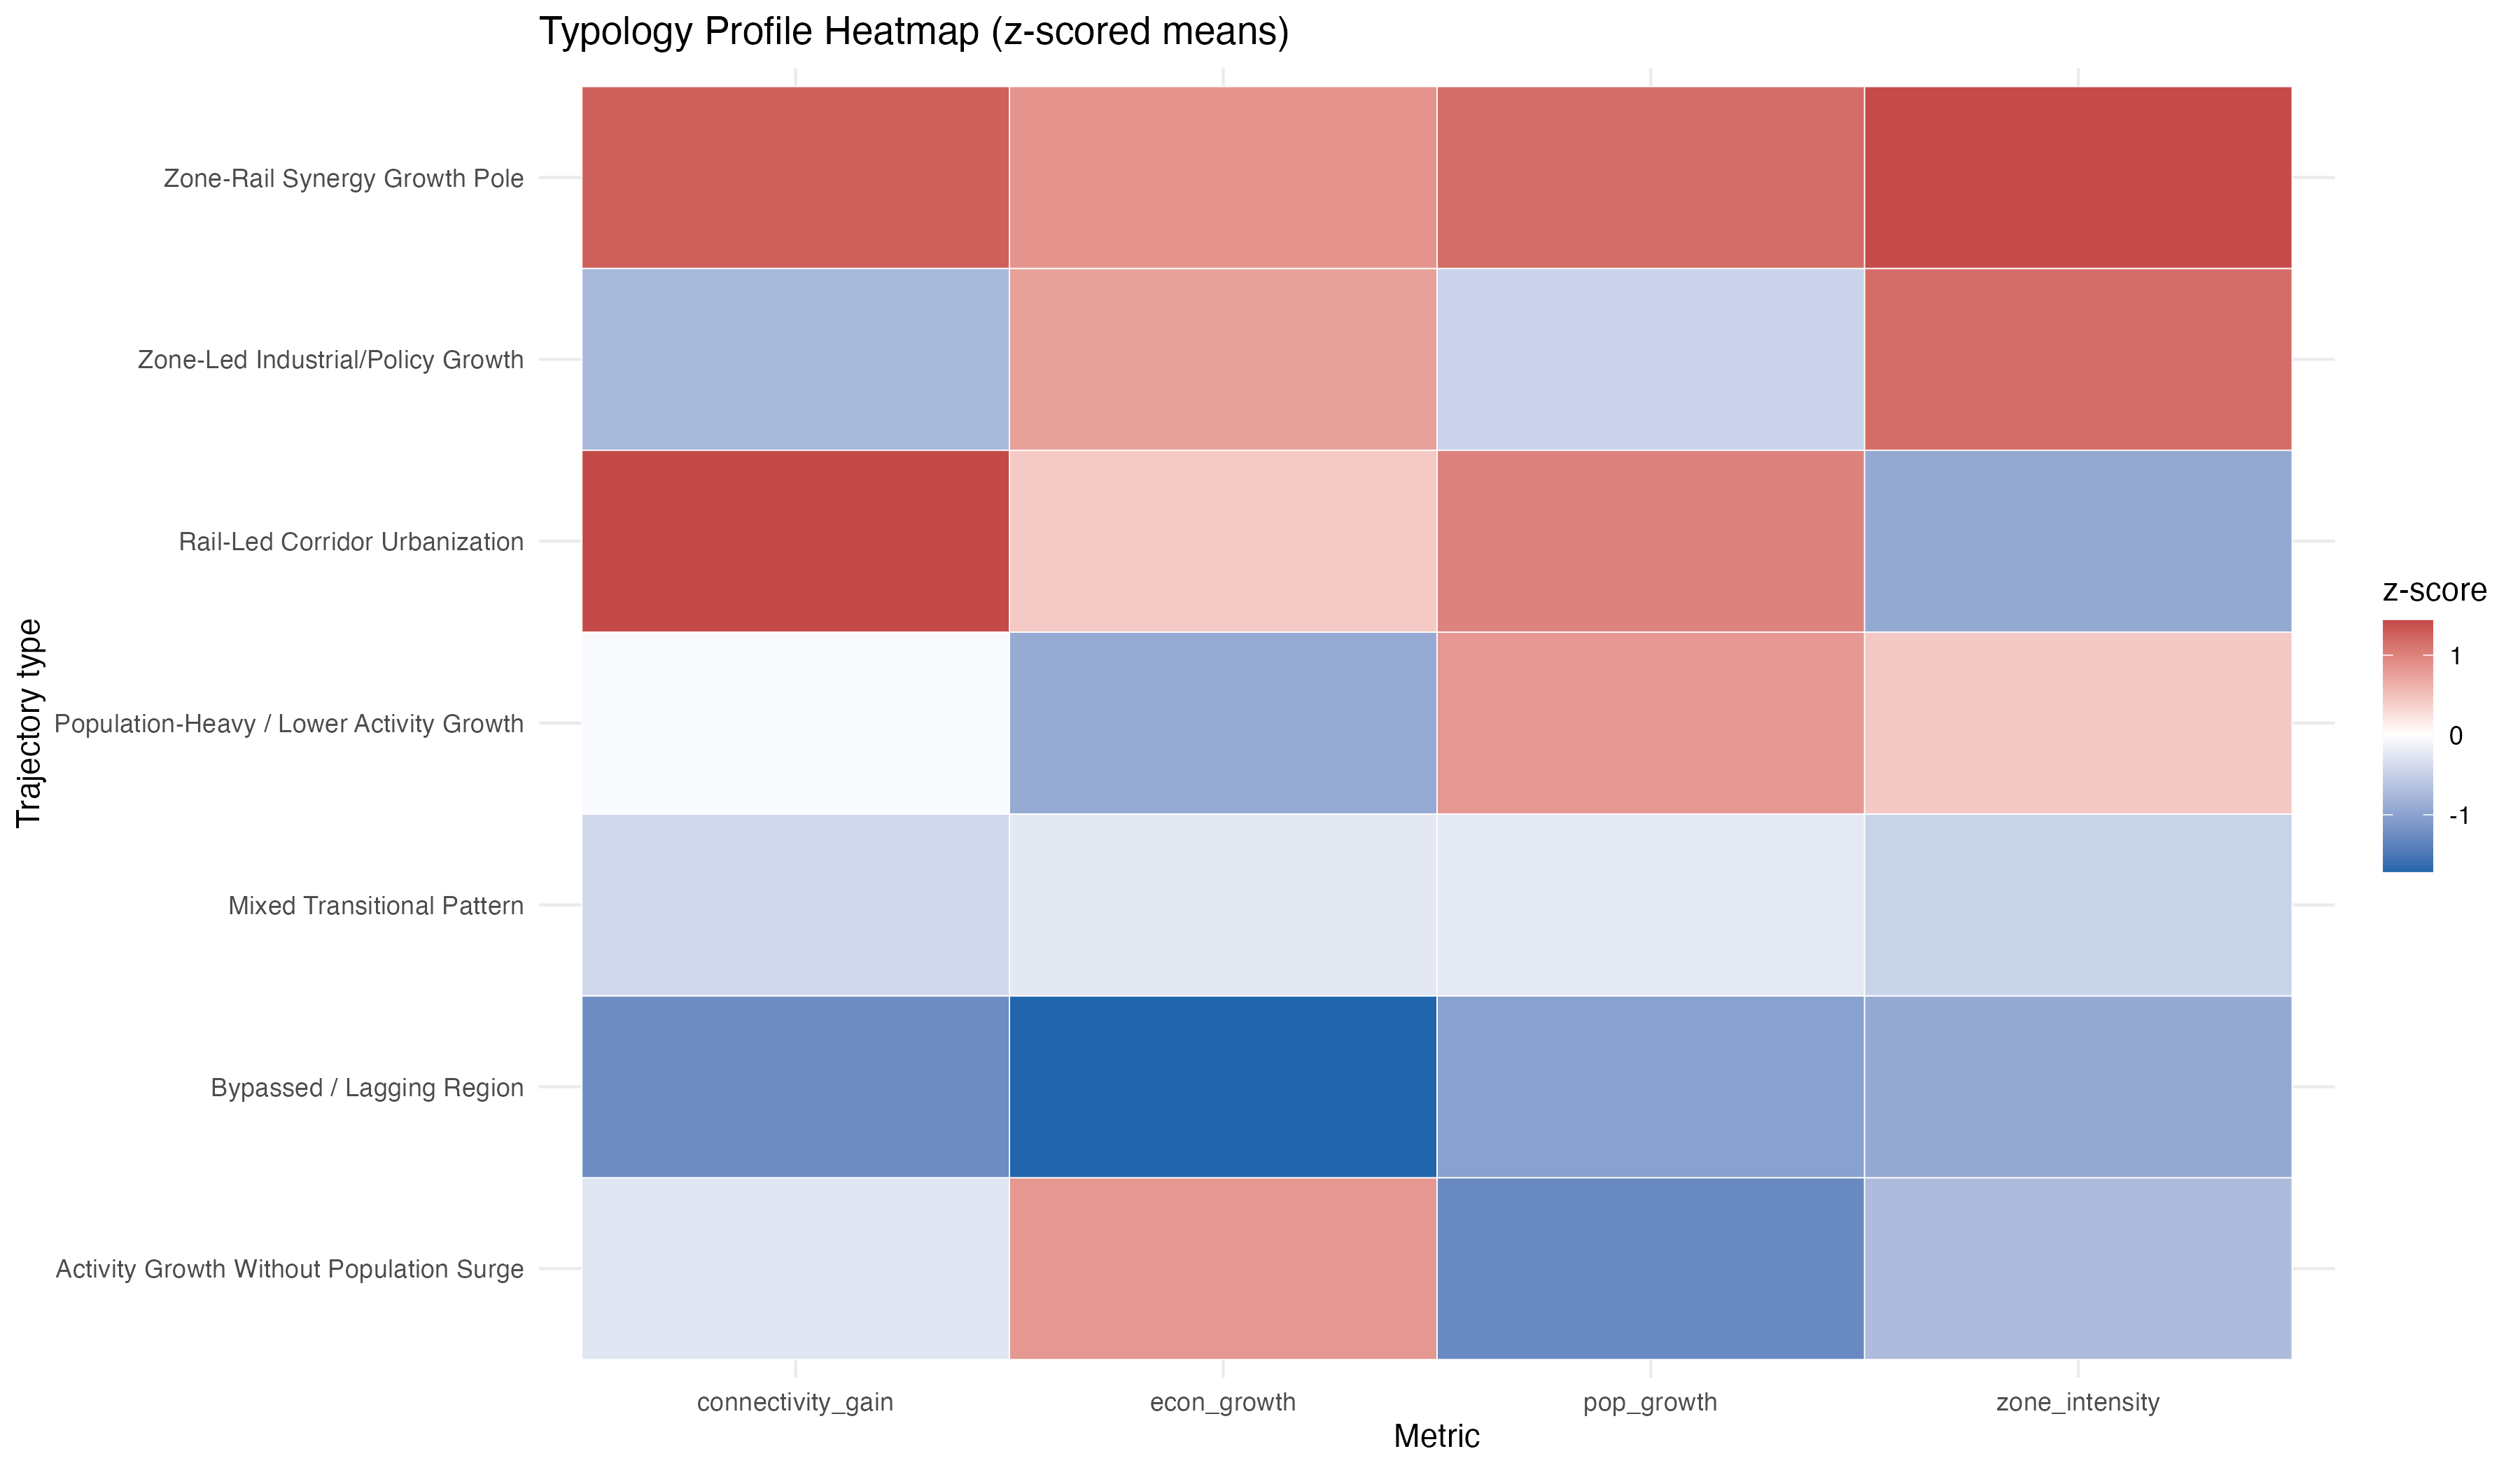
\includegraphics[width=\linewidth,height=0.76\textheight,keepaspectratio]{outputs/figures/fig_16_typology_metric_heatmap.png}
\end{columns}
\vspace{0.2em}
\small
Mixed Transitional Pattern dominates (58.72\%), while high-synergy poles are concentrated but limited in count (2.33\%).
\end{frame}

\begin{frame}{Corridor Gradient: Population Outcome}
\small
\begin{columns}[T,onlytextwidth]
\column{0.64\linewidth}
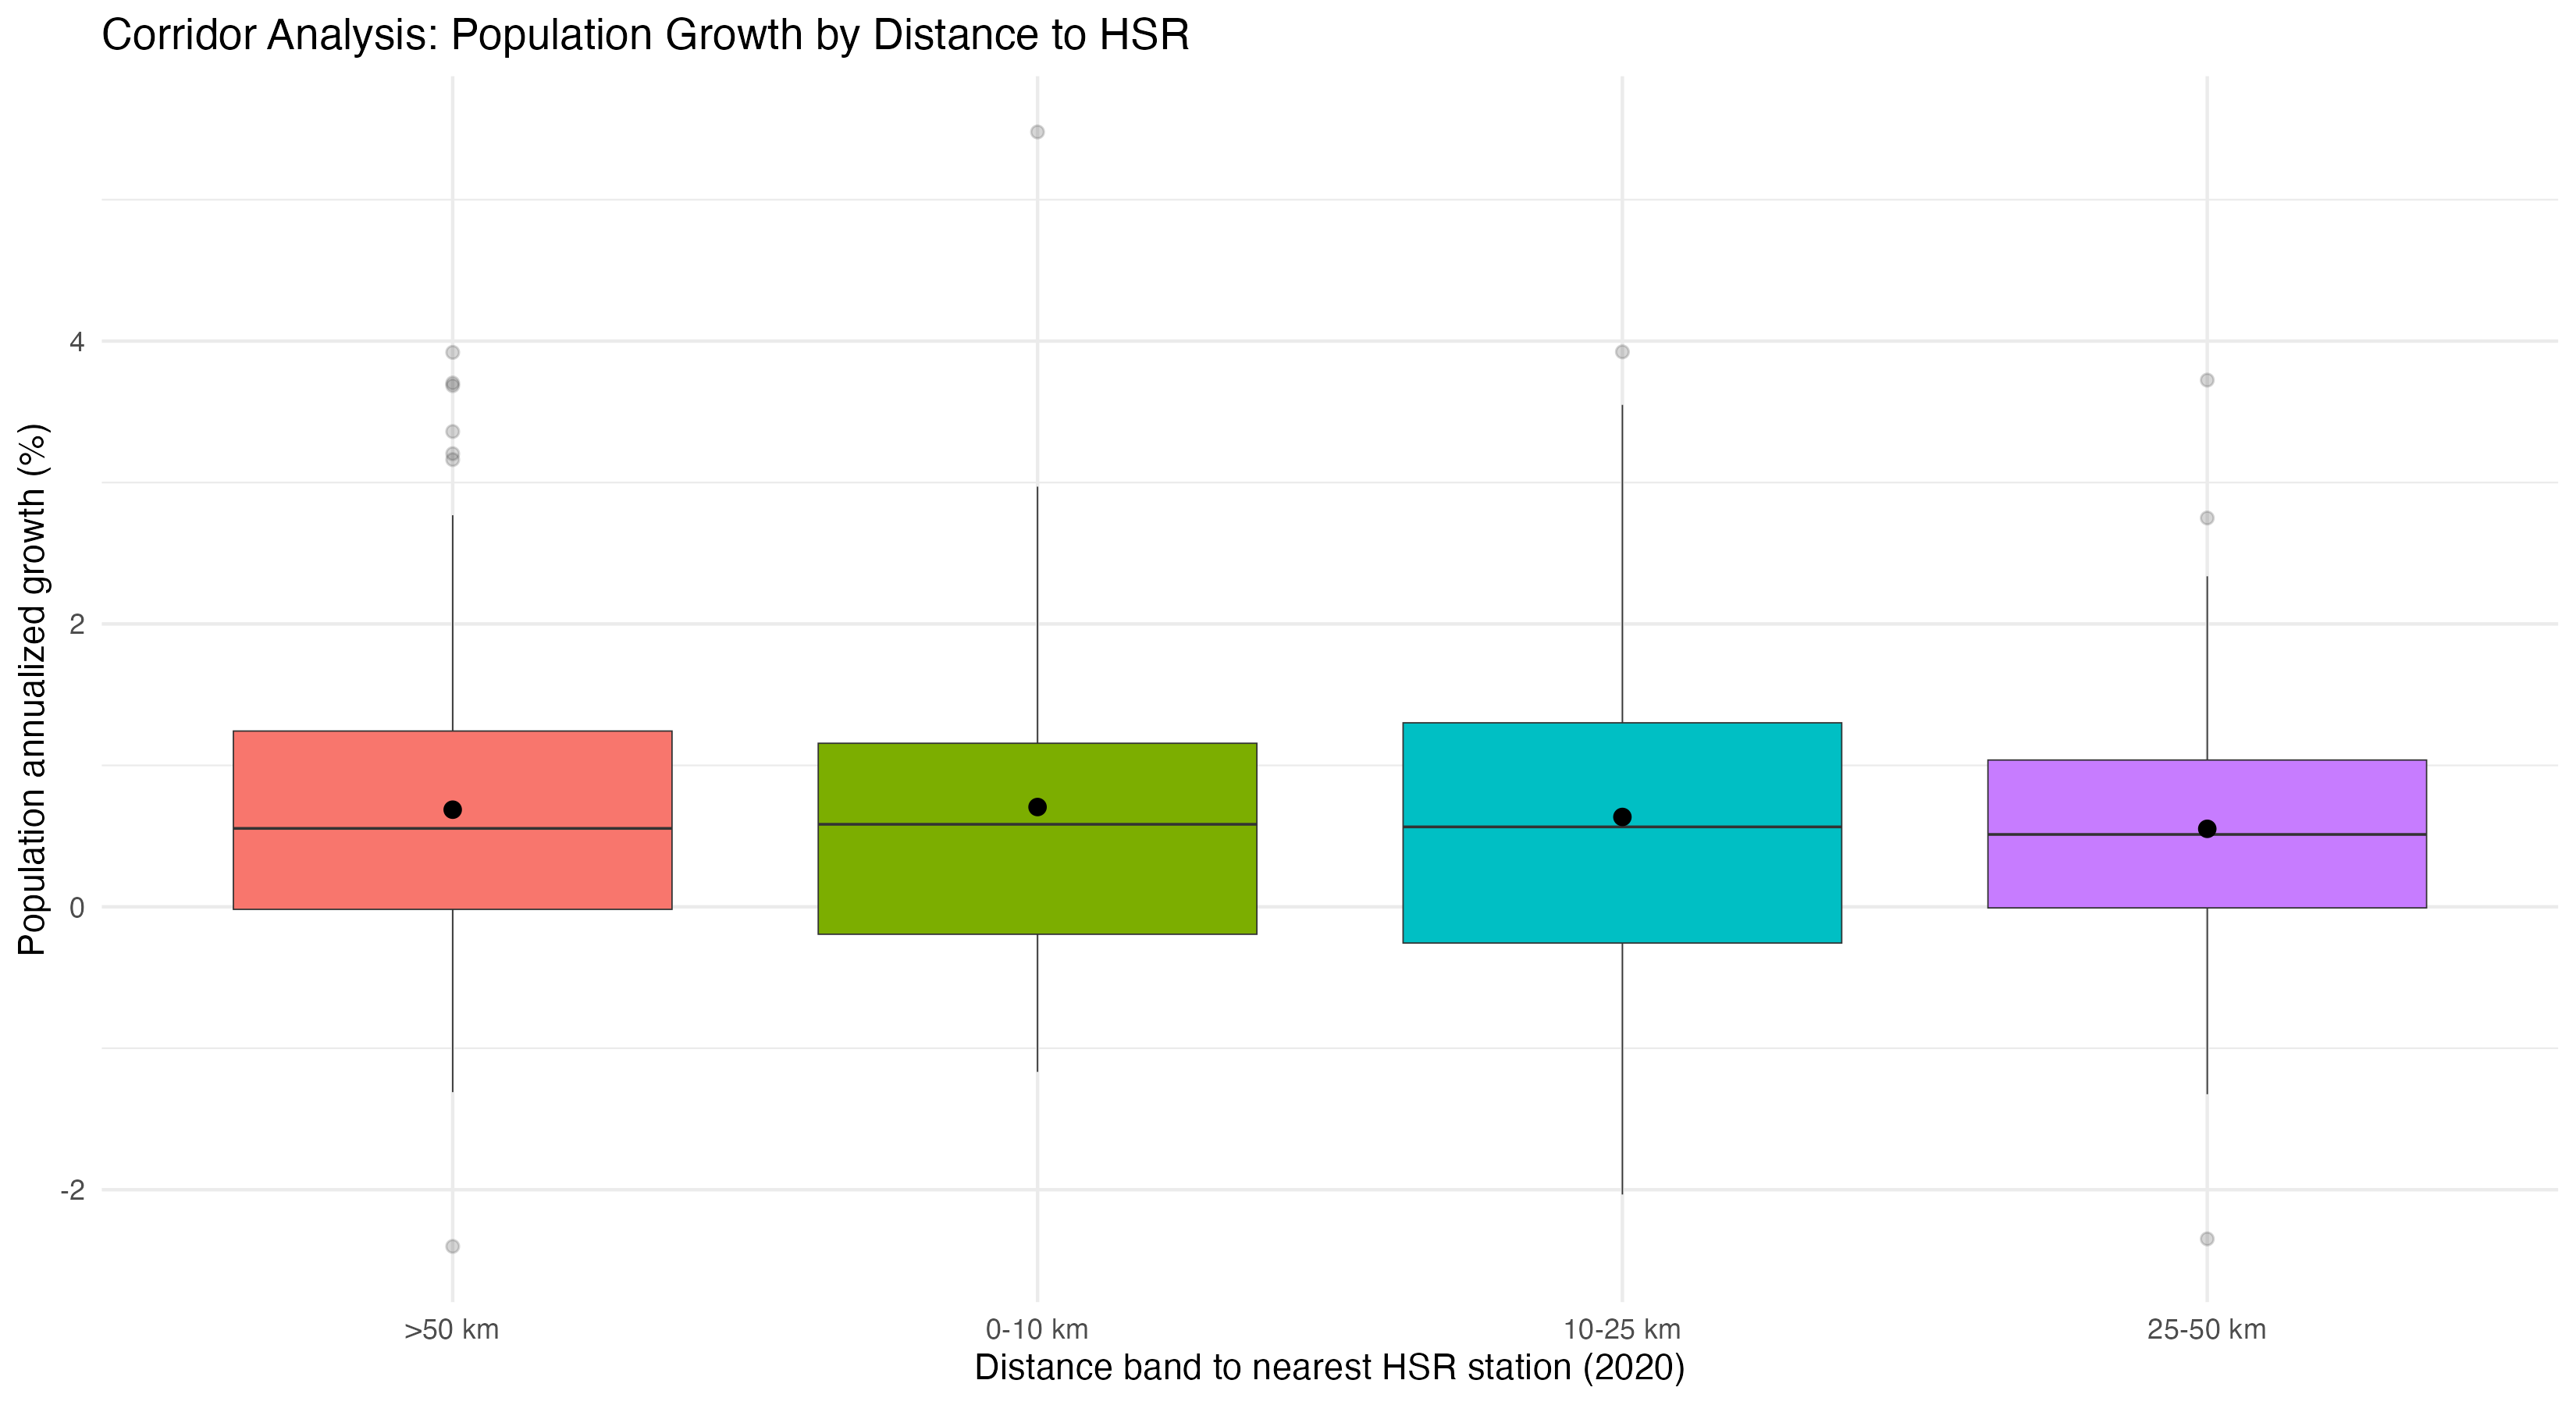
\includegraphics[width=\linewidth,height=0.74\textheight,keepaspectratio]{outputs/figures/fig_10_corridor_population_growth.png}
\column{0.34\linewidth}
\justifying
Near-far HSR gap (near $\leq$10 km vs far $>$50 km):
\begin{itemize}
  \item estimate: +0.019 pp/year
  \item 95\% CI: [-0.427, 0.478]
  \item permutation p-value: 0.921
\end{itemize}
\vspace{0.2em}
Interpretation: direction is positive but evidence is weak for a population-growth differential at this baseline threshold.
\end{columns}
\end{frame}

\begin{frame}{Corridor Gradient: Economic Outcome}
\small
\begin{columns}[T,onlytextwidth]
\column{0.64\linewidth}
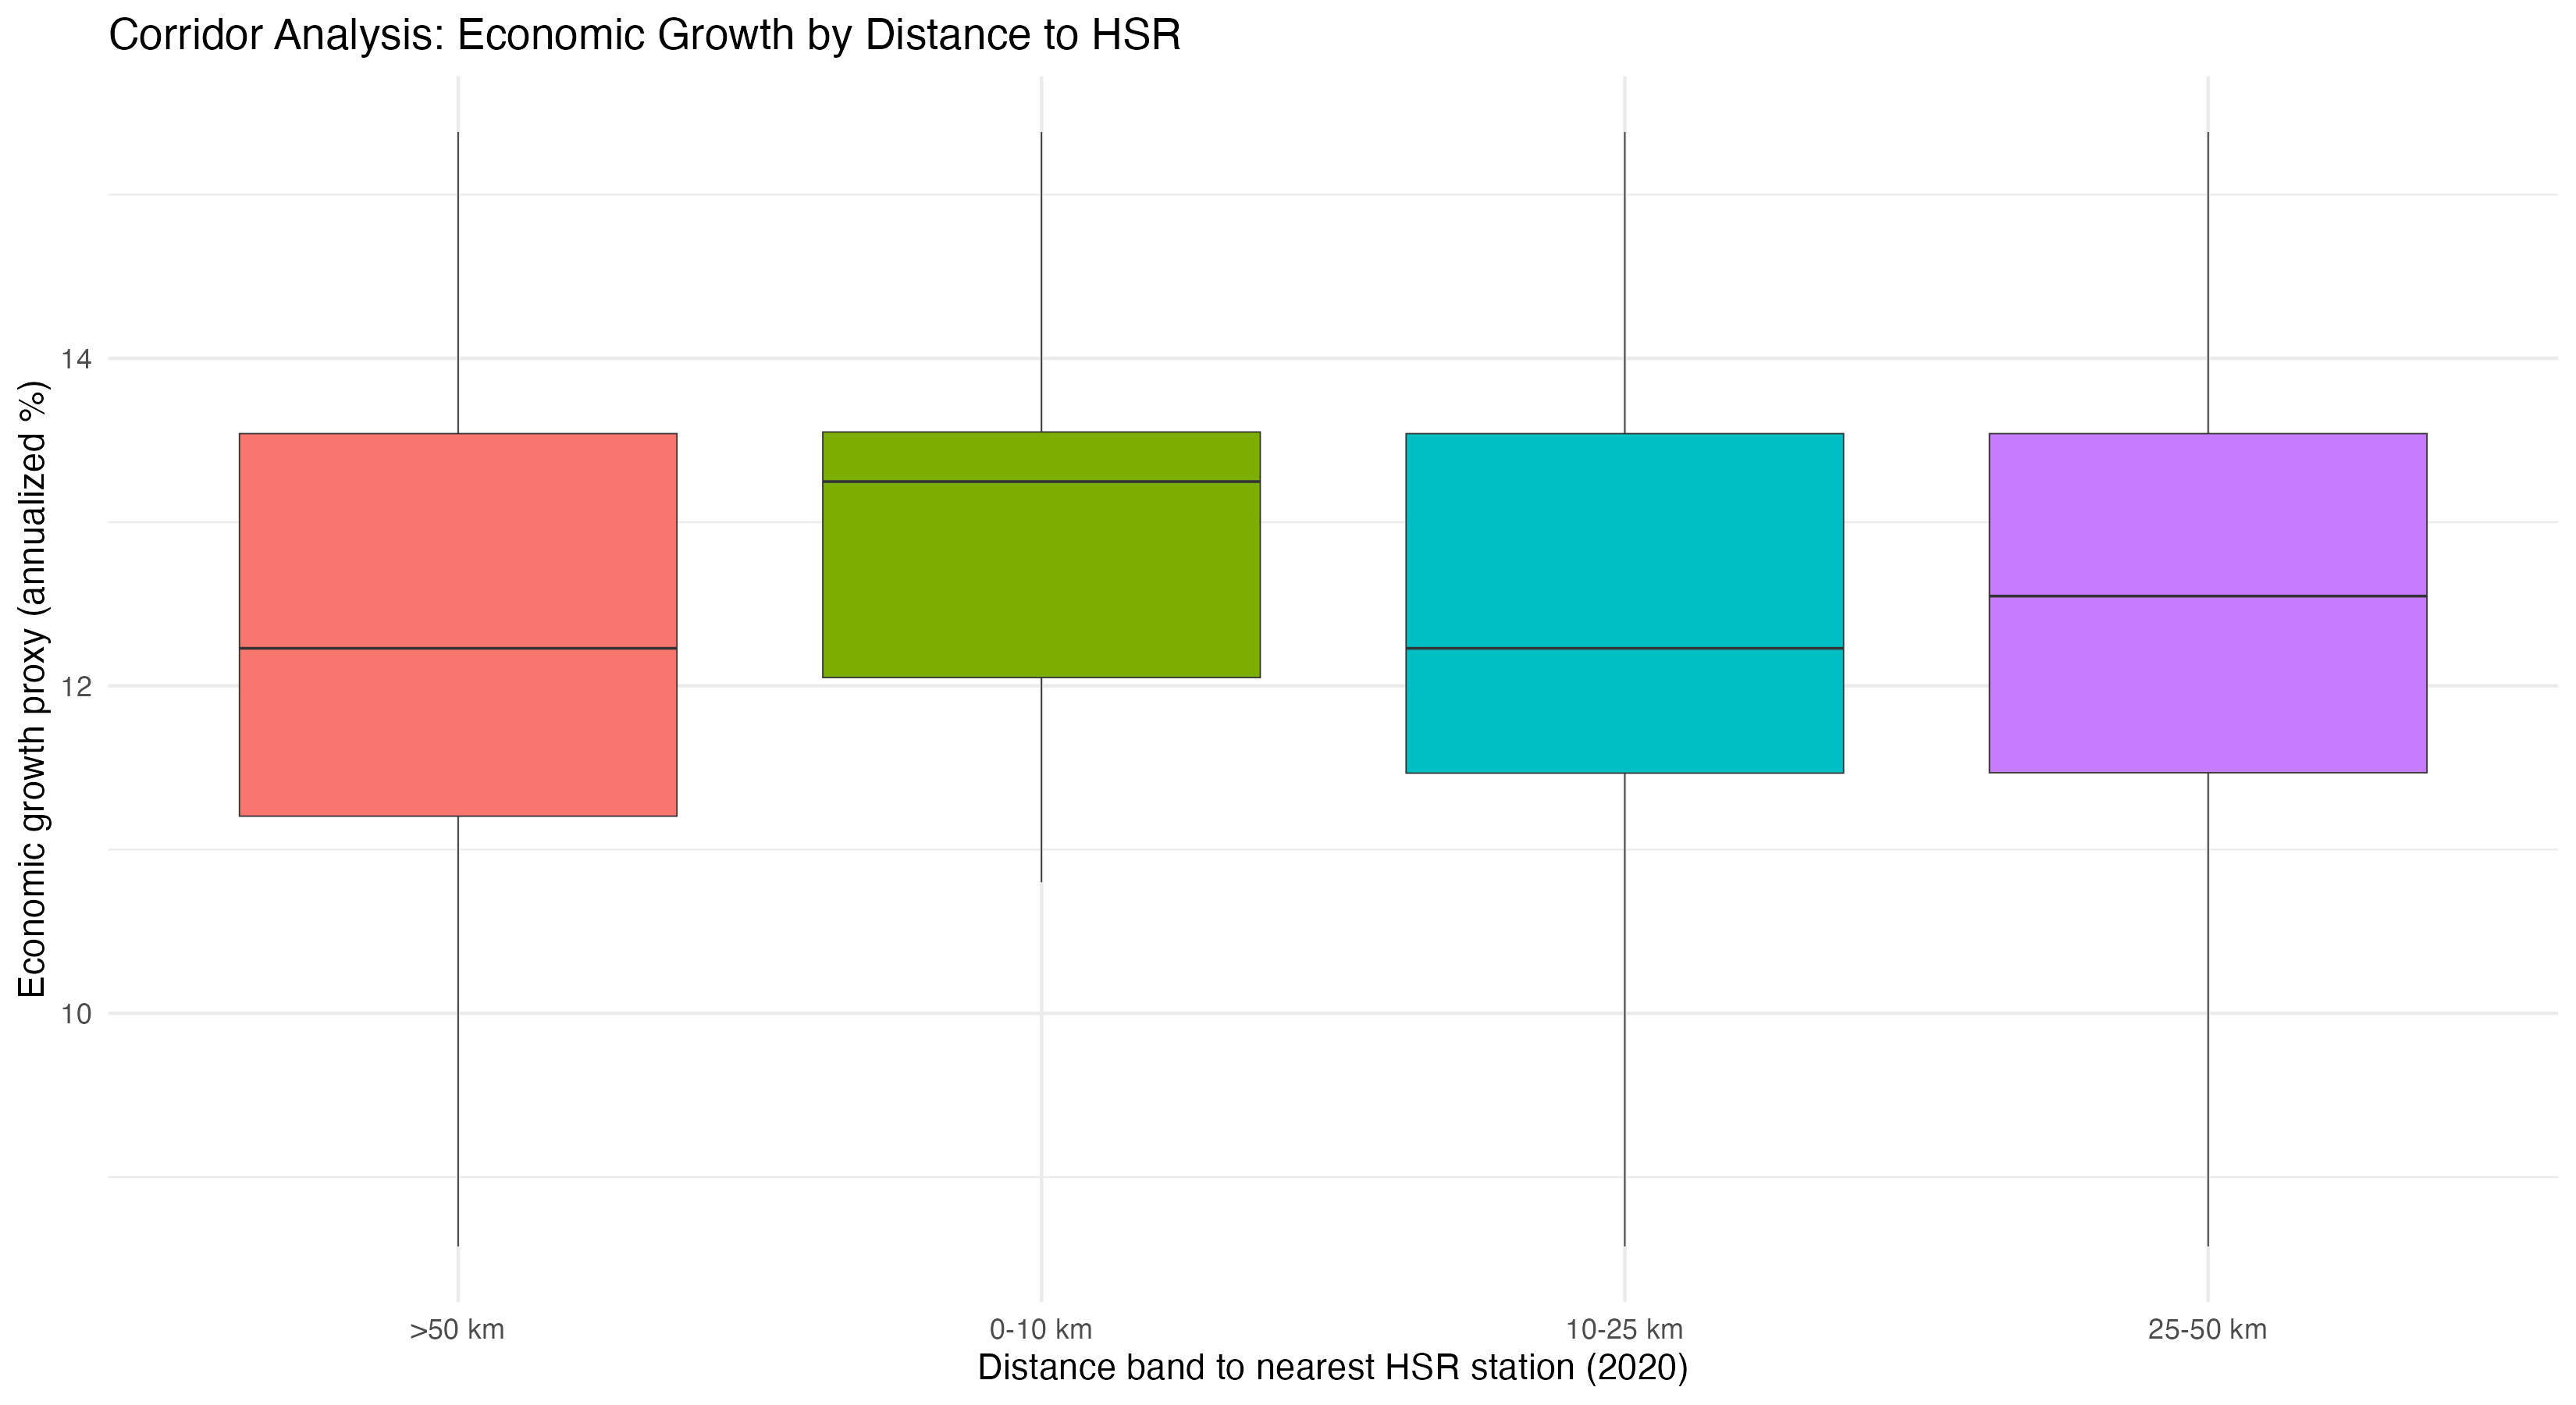
\includegraphics[width=\linewidth,height=0.74\textheight,keepaspectratio]{outputs/figures/fig_11_corridor_econ_growth.png}
\column{0.34\linewidth}
\justifying
Near-far HSR gap (near $\leq$10 km vs far $>$50 km):
\begin{itemize}
  \item estimate: +0.762 pp/year
  \item 95\% CI: [0.302, 1.263]
  \item permutation p-value: 0.011
\end{itemize}
\vspace{0.2em}
Interpretation: economically meaningful and statistically robust association in the baseline corridor contrast.
\end{columns}
\end{frame}

\begin{frame}{Threshold Sensitivity of Near-Far Gaps}
\centering
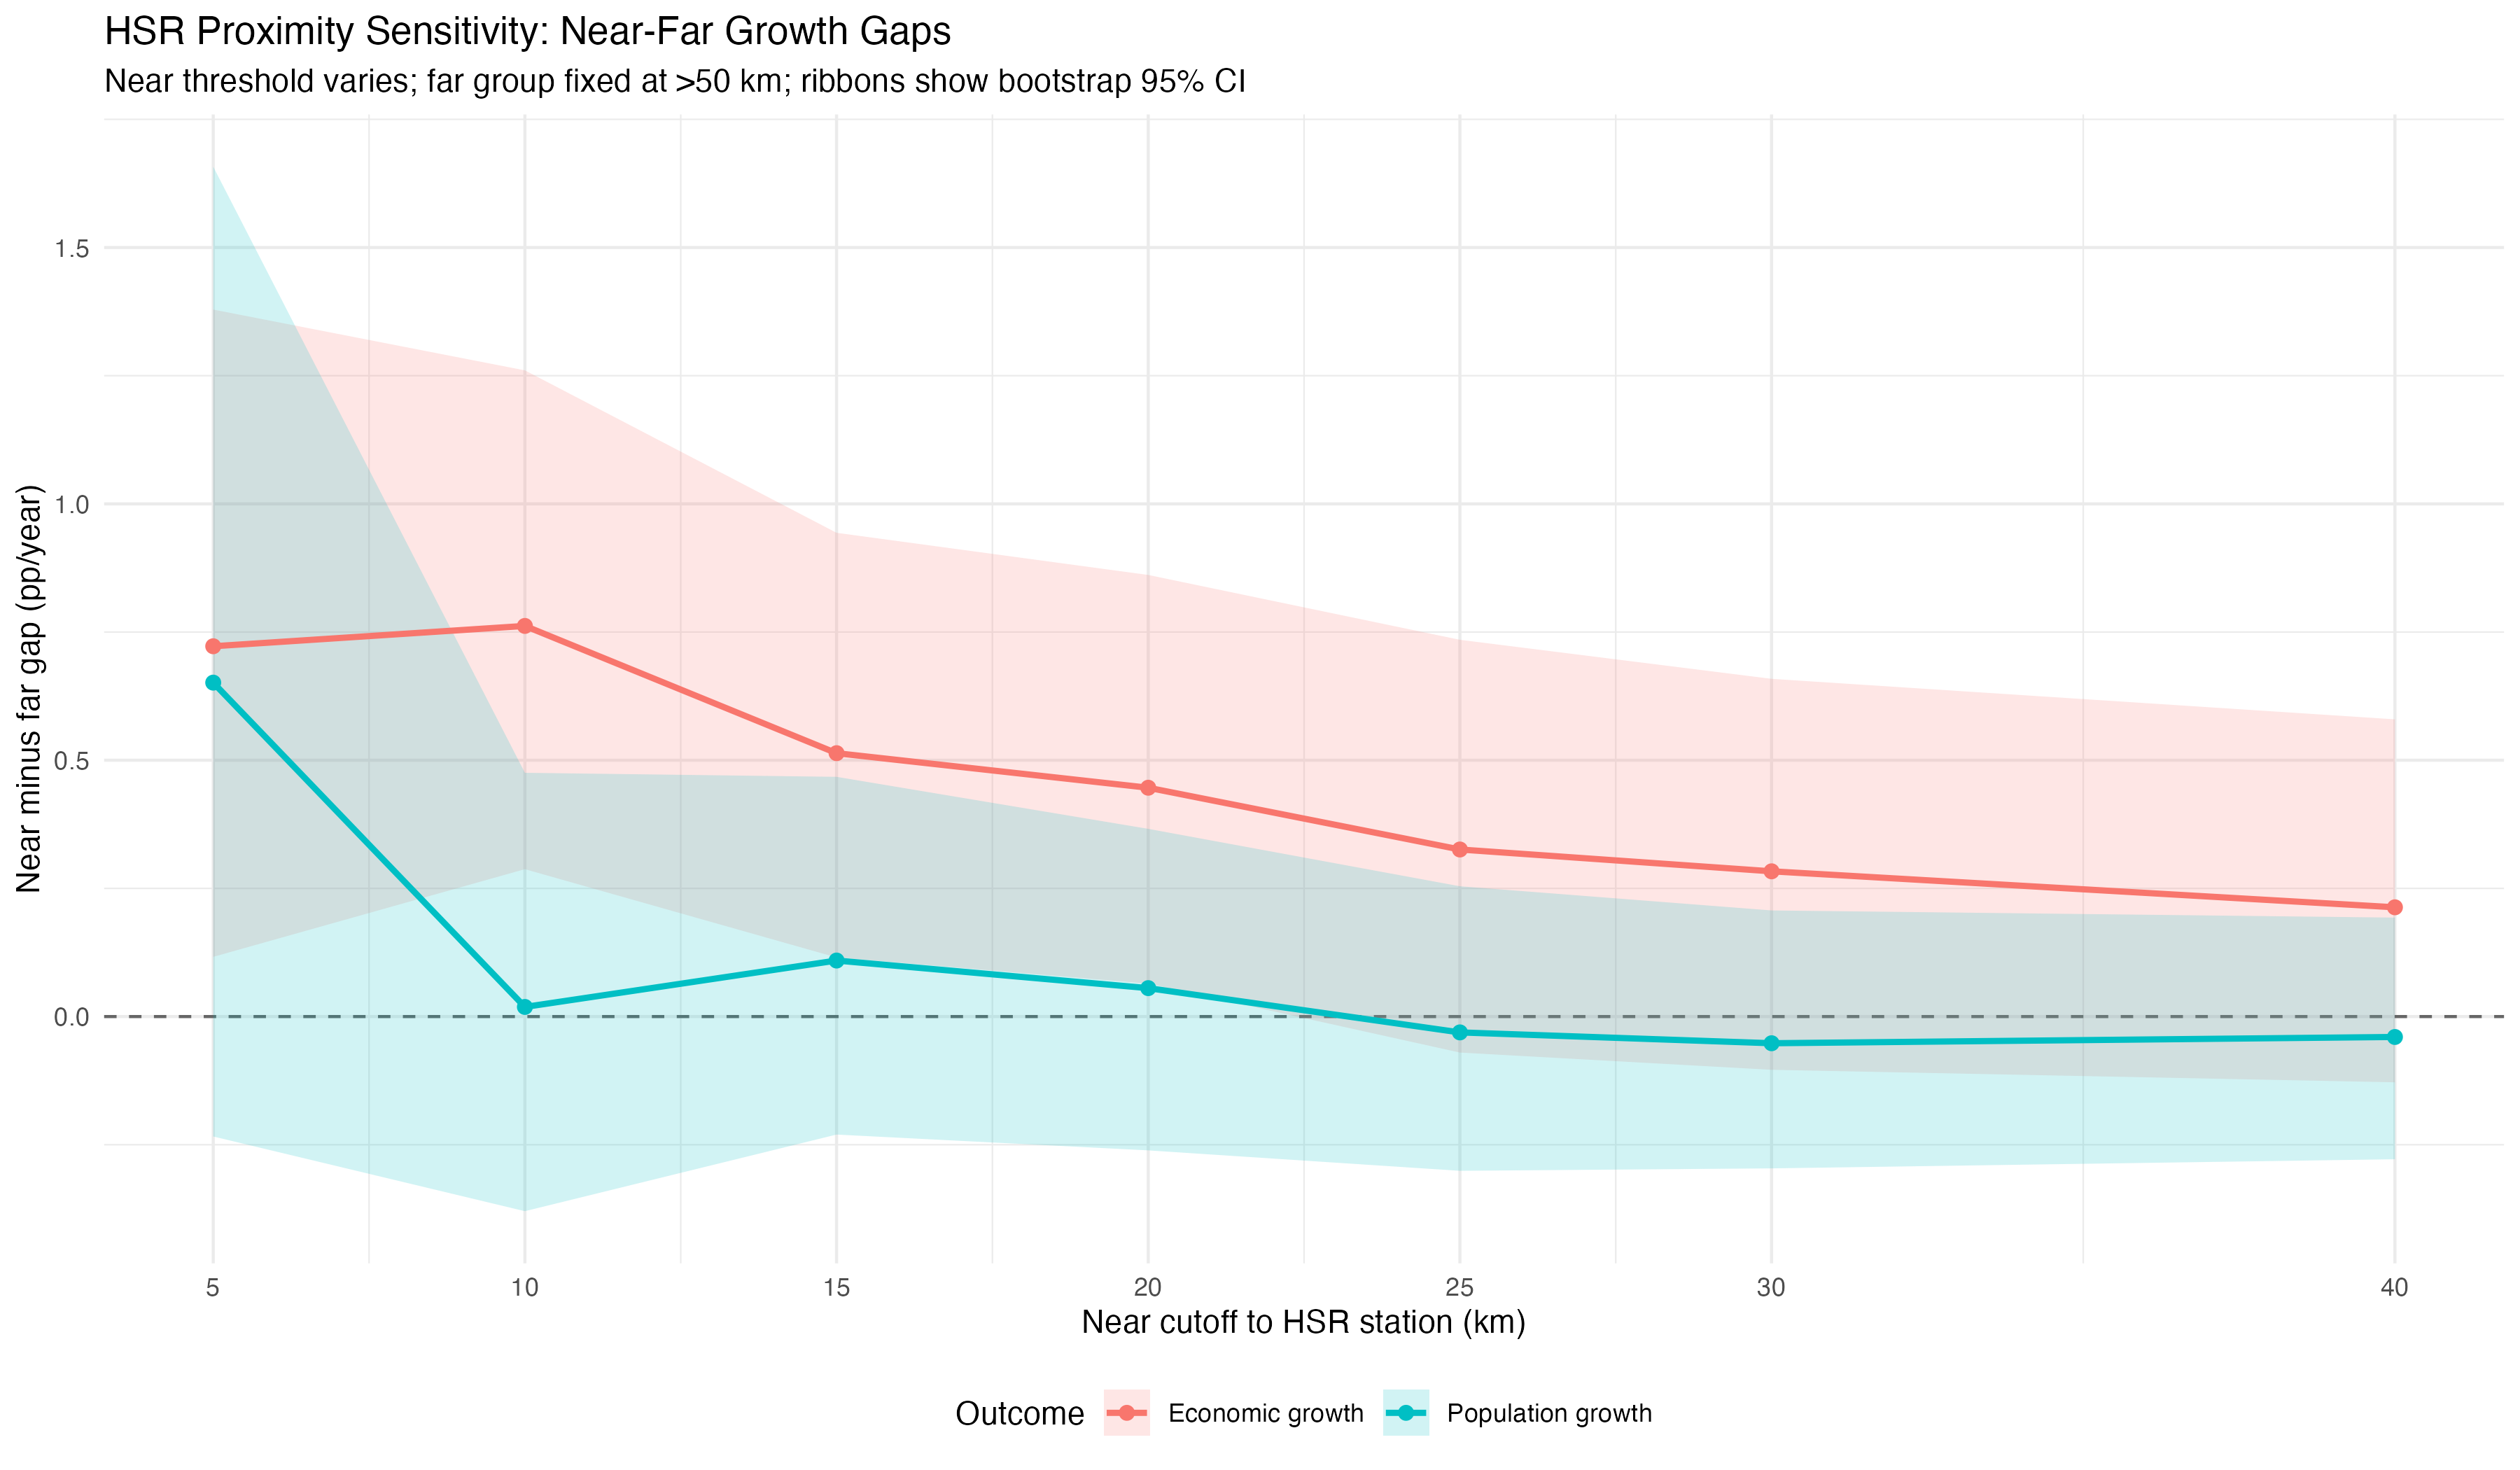
\includegraphics[width=0.97\linewidth,height=0.82\textheight,keepaspectratio]{outputs/figures/fig_23_hsr_threshold_sensitivity.png}
\end{frame}

\begin{frame}{Adjusted Driver Associations}
\centering
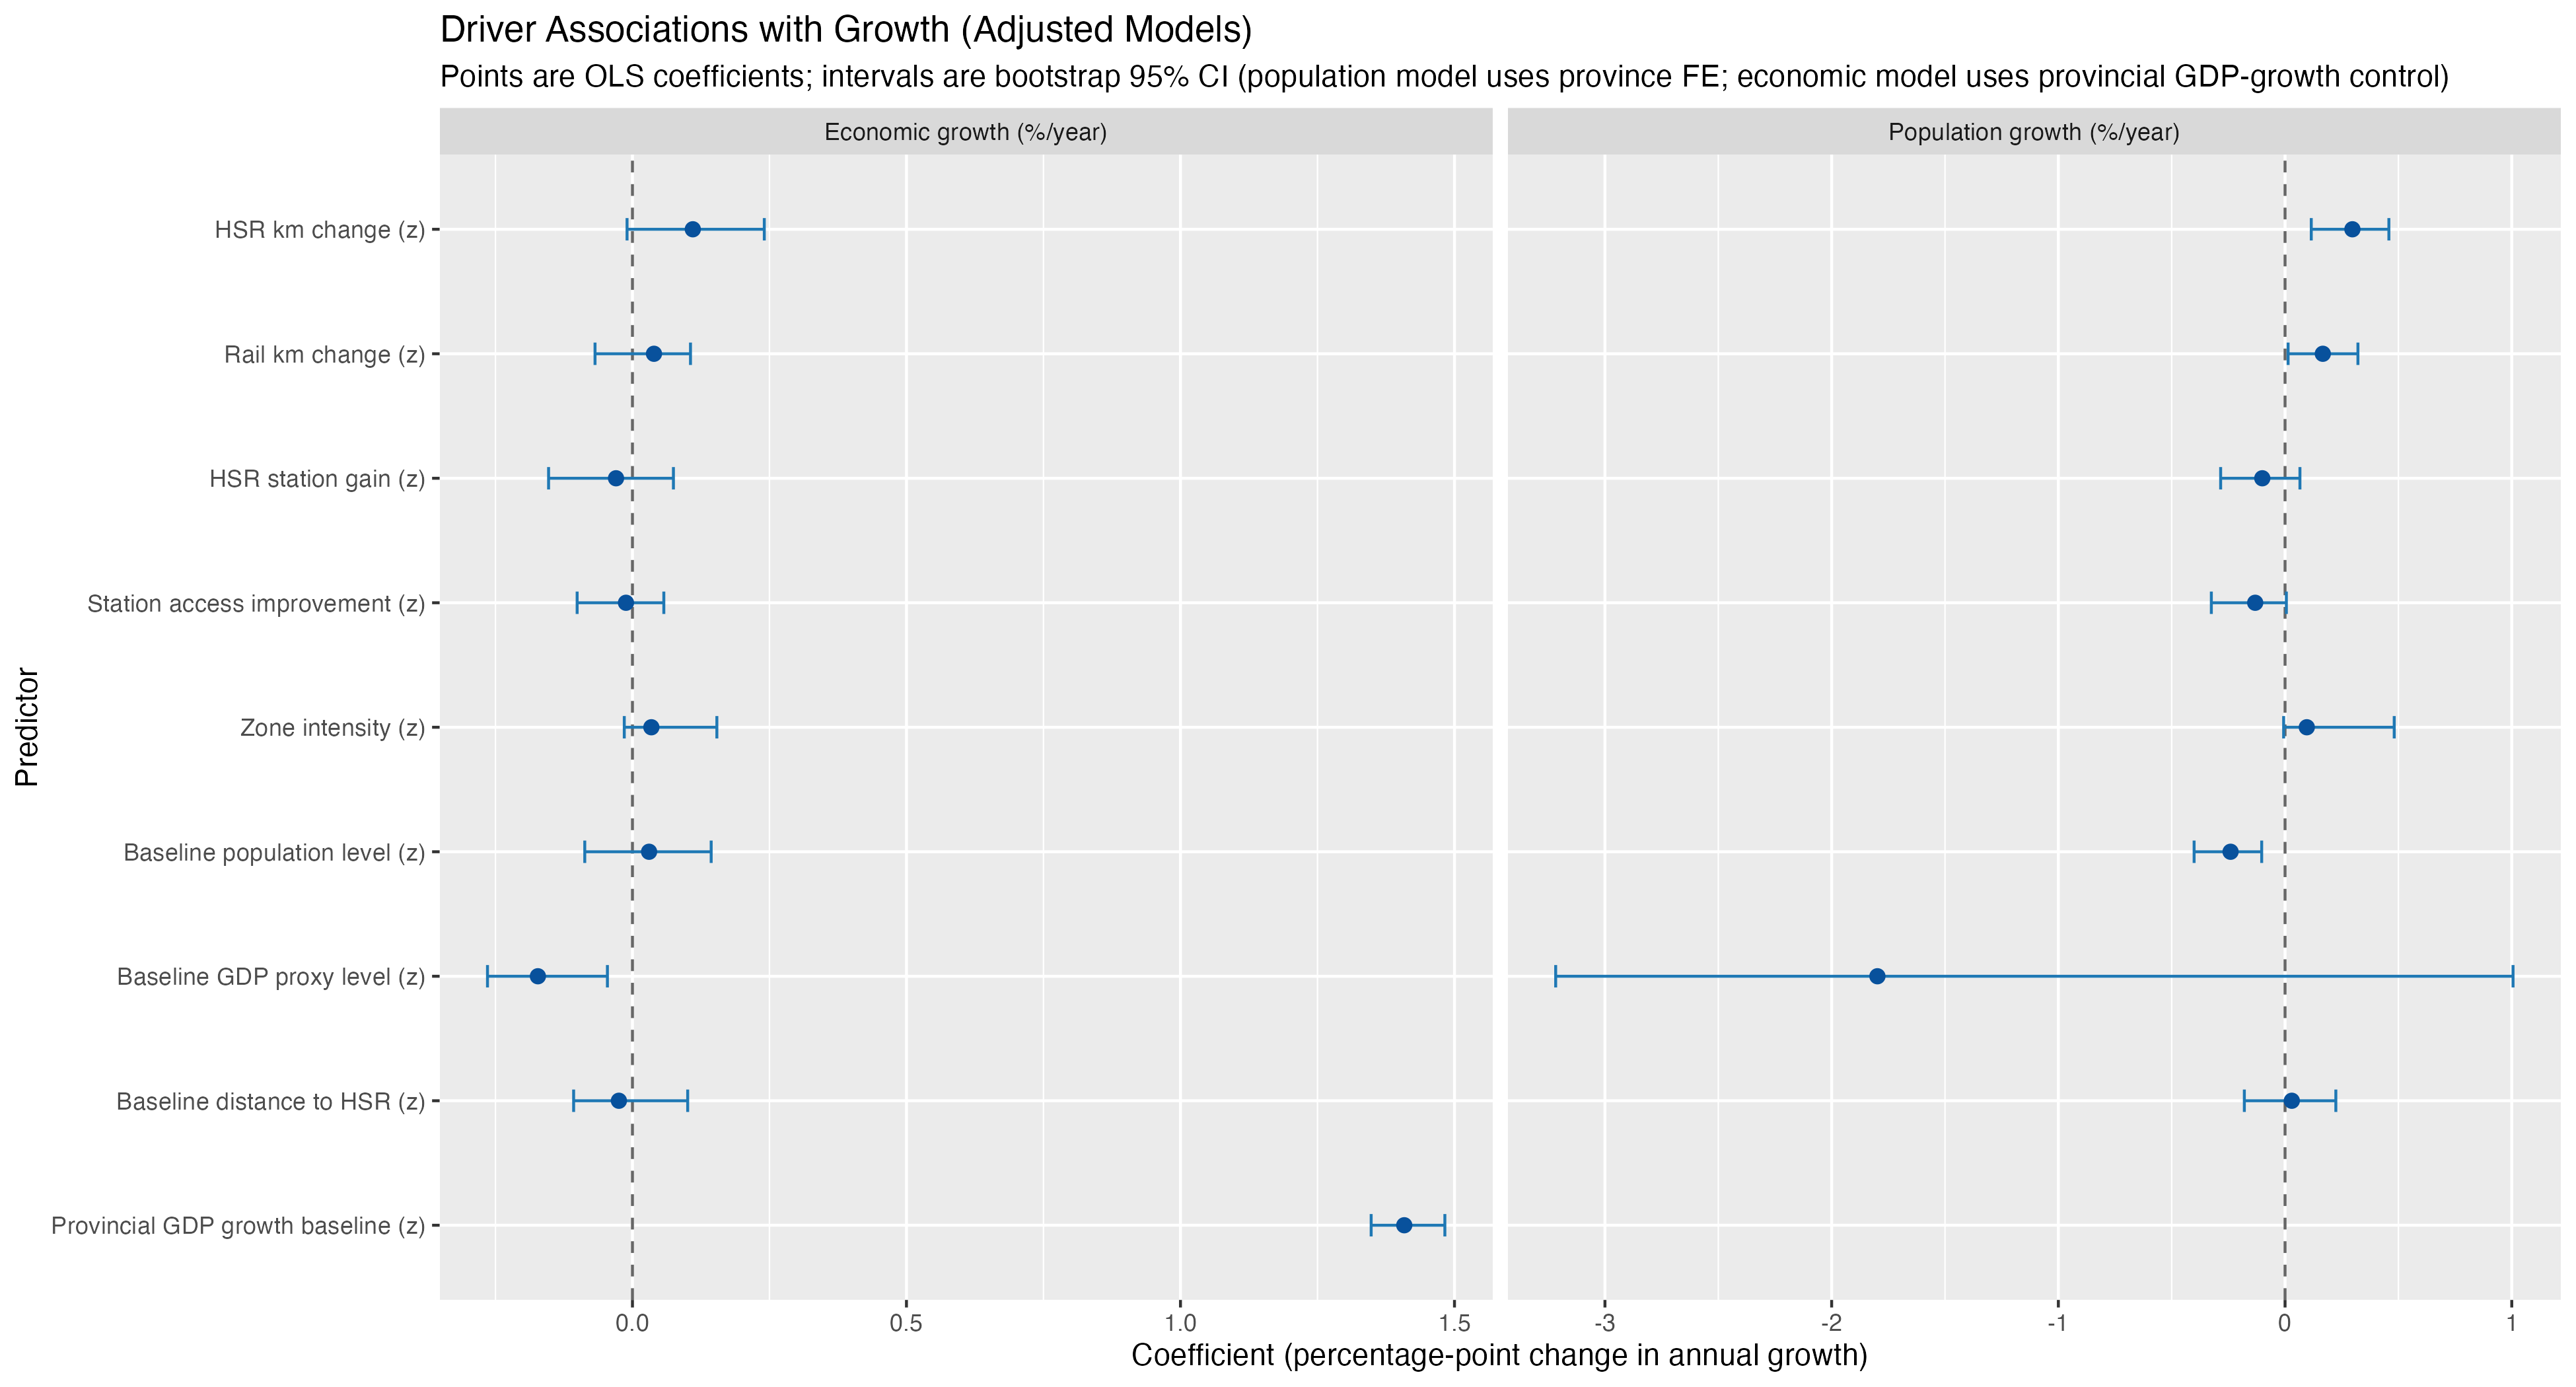
\includegraphics[width=0.97\linewidth,height=0.82\textheight,keepaspectratio]{outputs/figures/fig_24_driver_coefficients_bootstrap.png}
\end{frame}

\begin{frame}{Concentration Dynamics and Distribution Shape}
\small
\begin{columns}[T,onlytextwidth]
\column{0.49\linewidth}
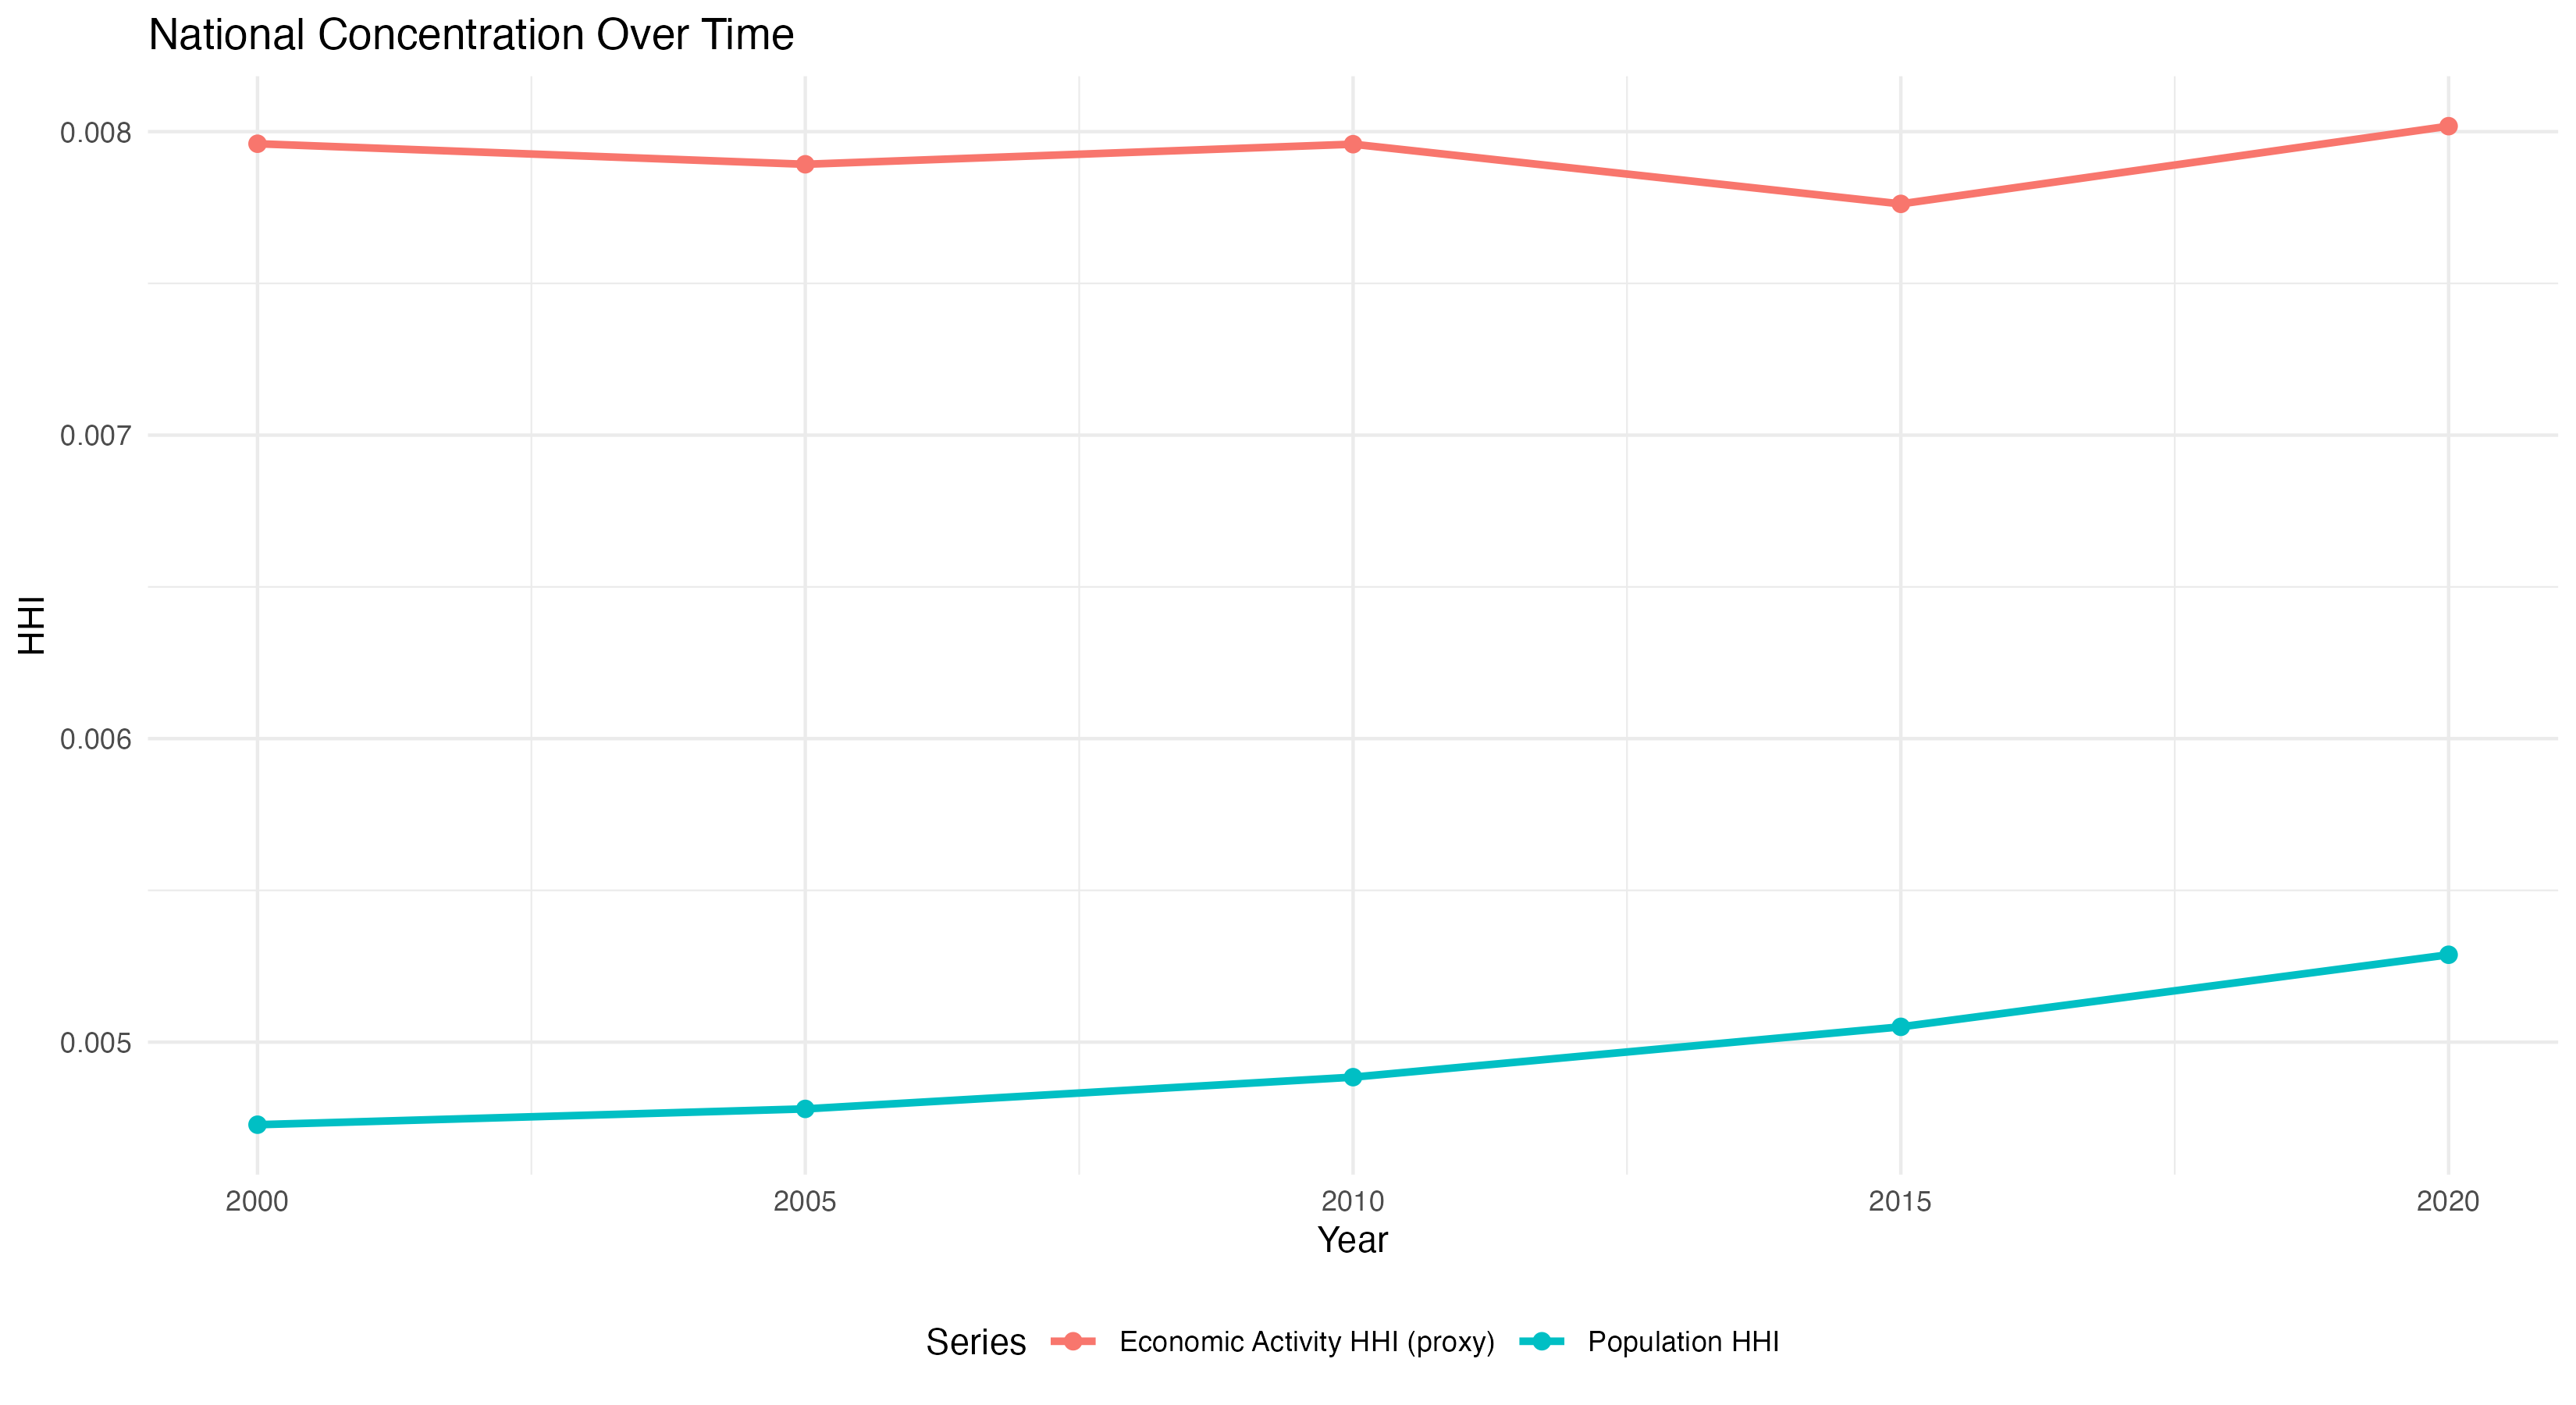
\includegraphics[width=\linewidth,height=0.72\textheight,keepaspectratio]{outputs/figures/fig_08_concentration_trends.png}
\column{0.49\linewidth}
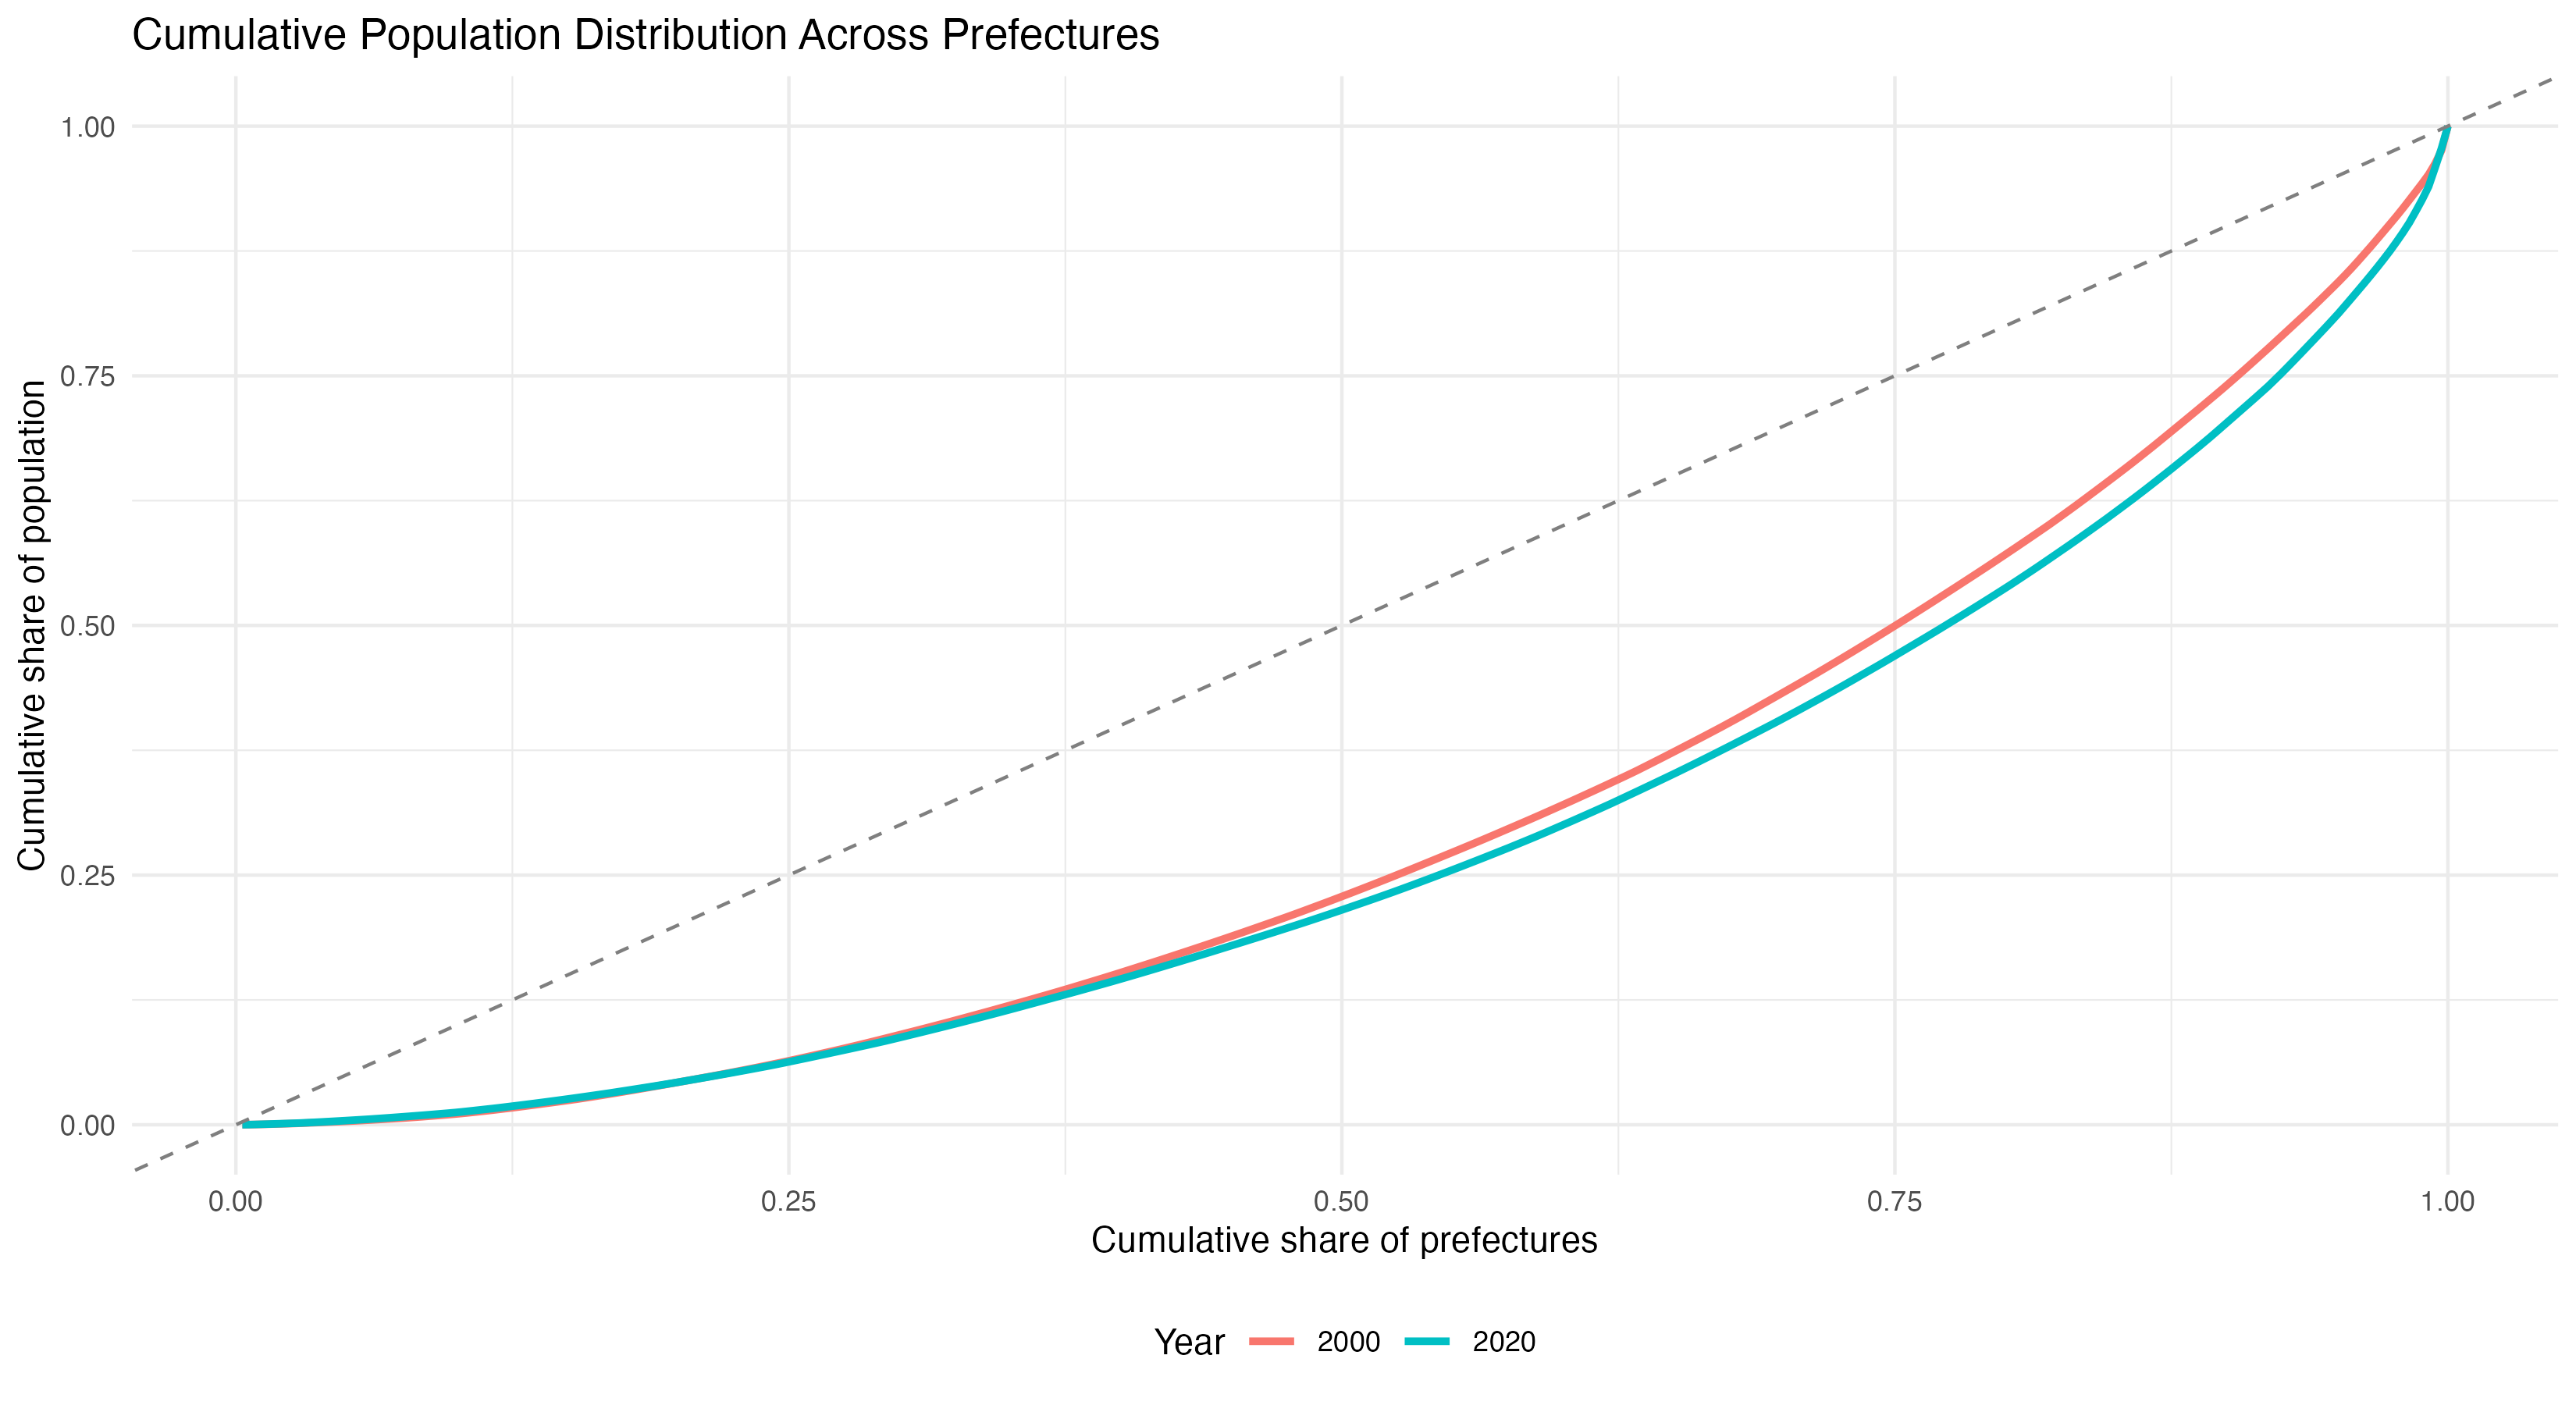
\includegraphics[width=\linewidth,height=0.72\textheight,keepaspectratio]{outputs/figures/fig_21_lorenz_population_distribution.png}
\end{columns}
\small
Population concentration rose by 11.84\% (HHI), while economic-proxy concentration changed only +0.73\%, indicating stronger demographic concentration than economic concentration in this panel setup.
\end{frame}

\begin{frame}{Cross-Metric Correlation Structure}
\small
\begin{columns}[T,onlytextwidth]
\column{0.5\linewidth}
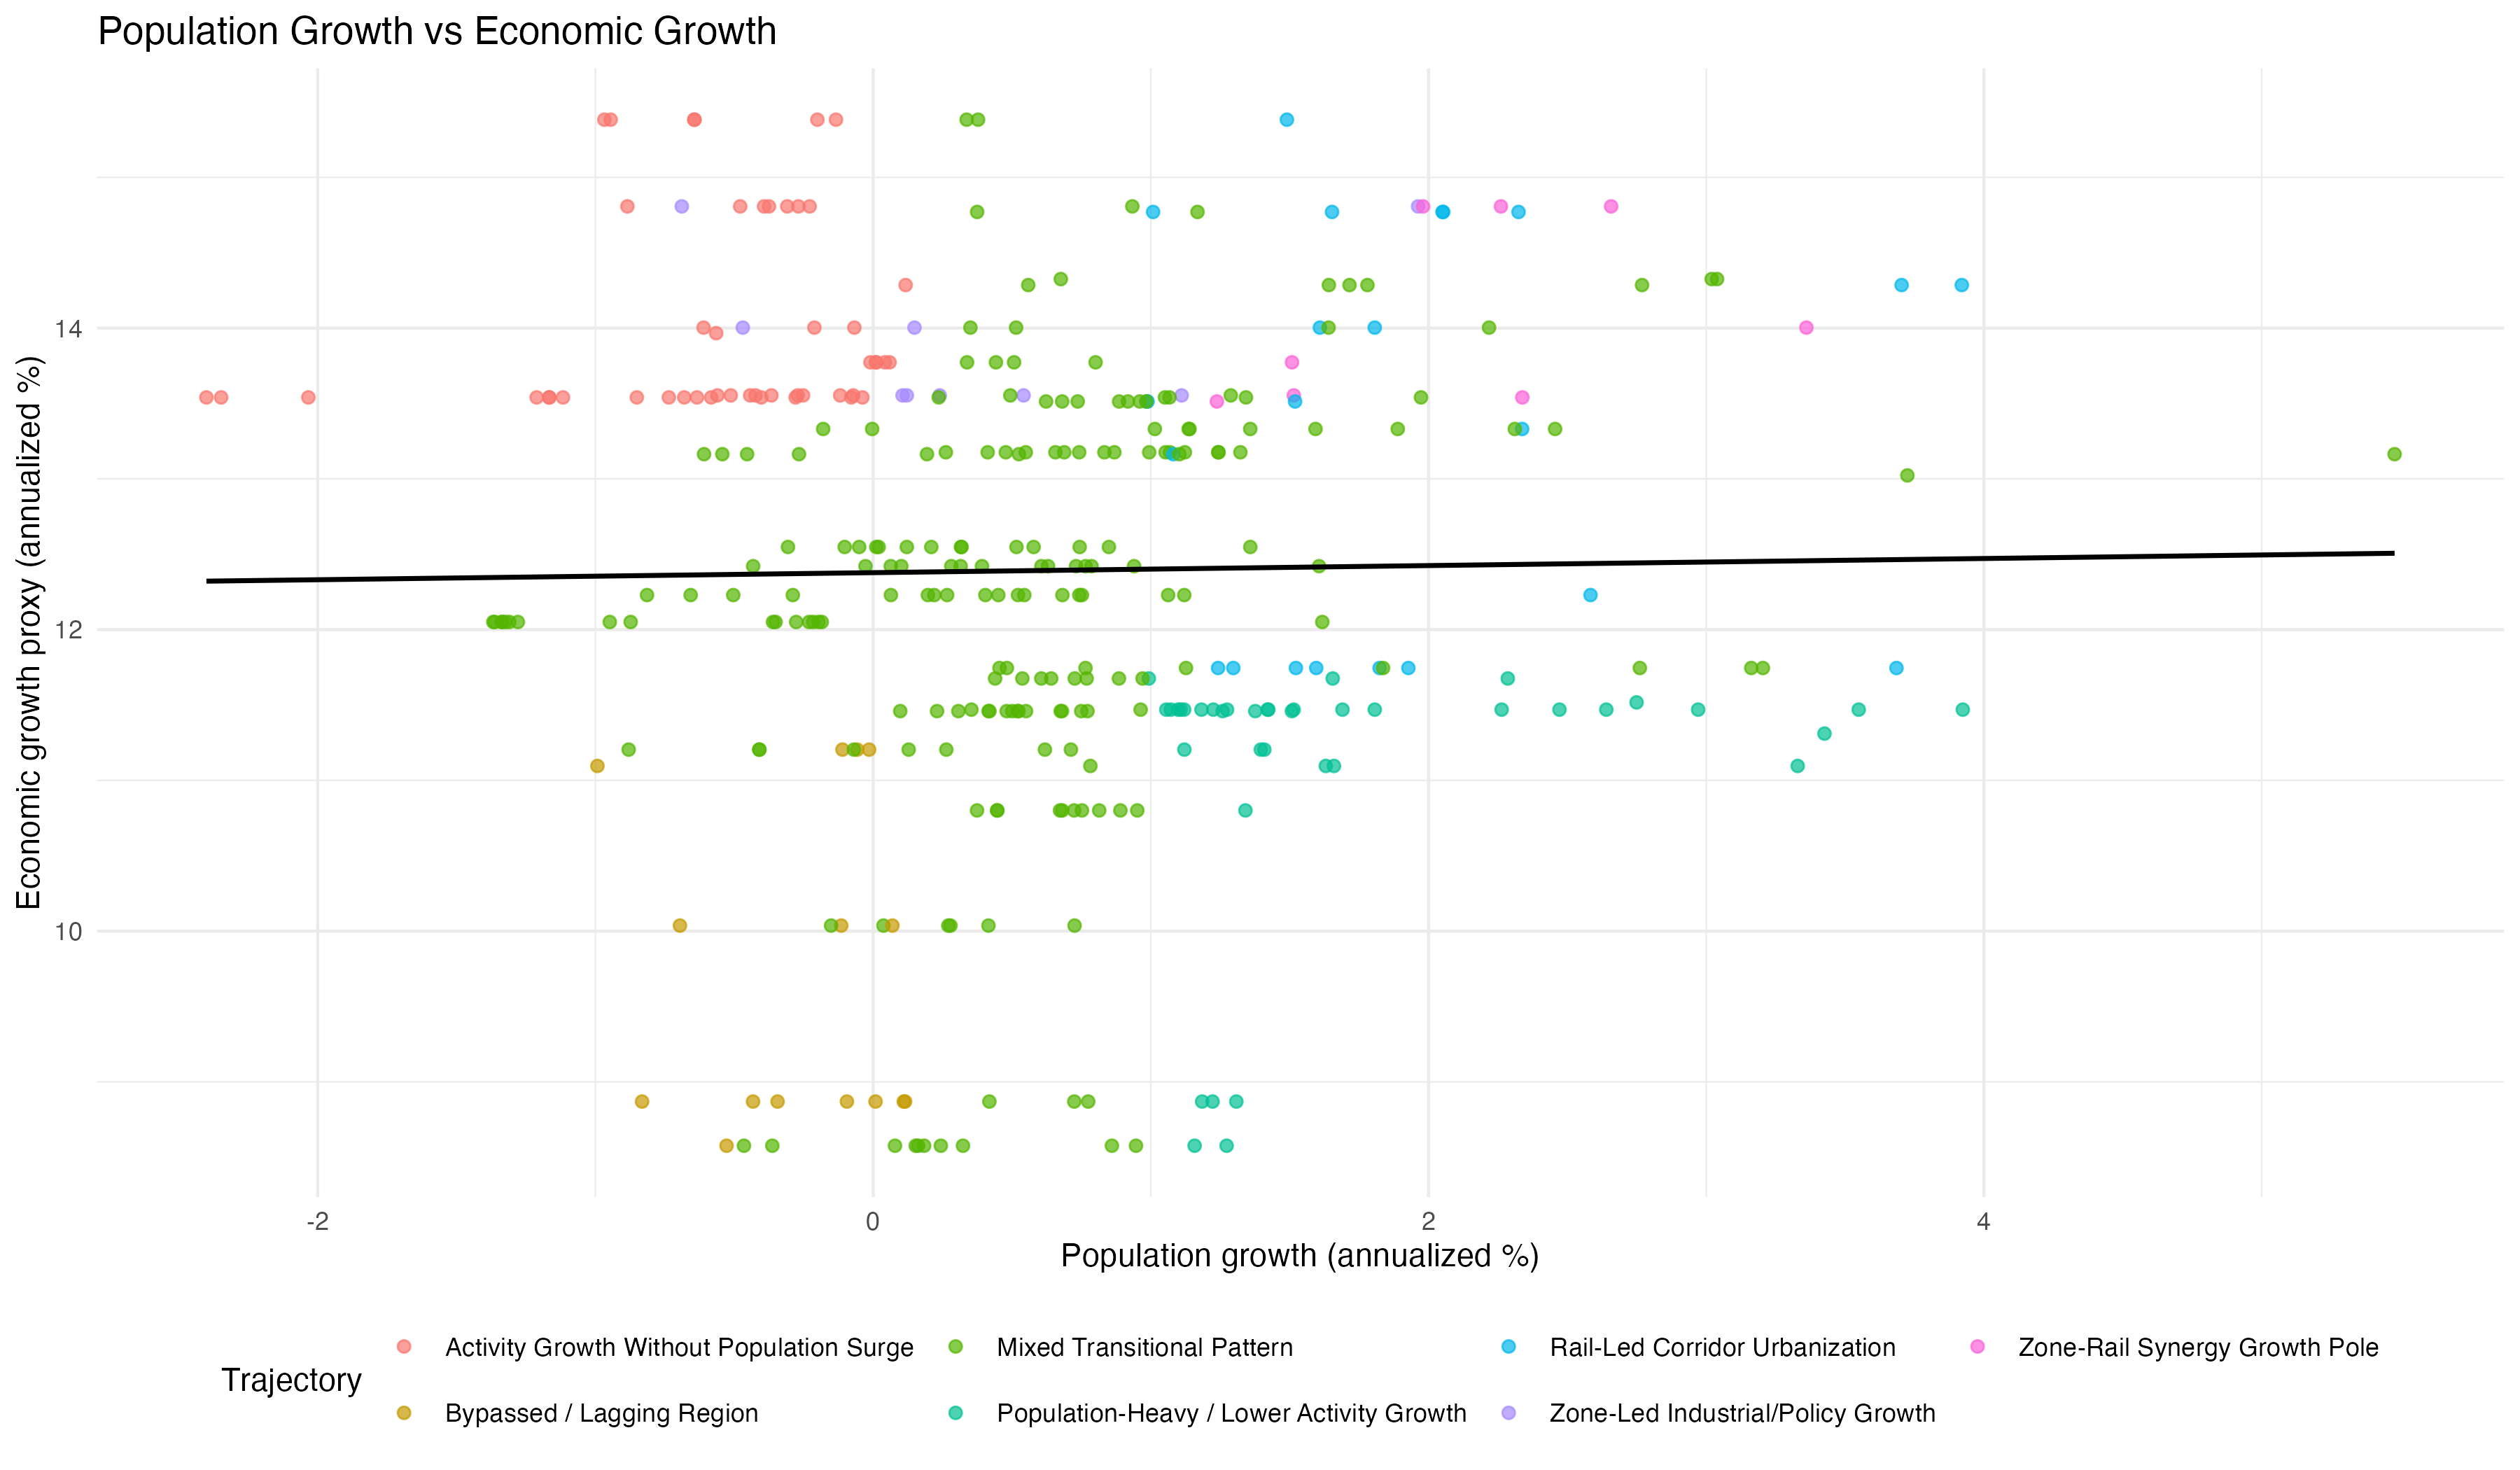
\includegraphics[width=\linewidth,height=0.72\textheight,keepaspectratio]{outputs/figures/fig_12_scatter_pop_vs_econ_growth.png}
\column{0.5\linewidth}
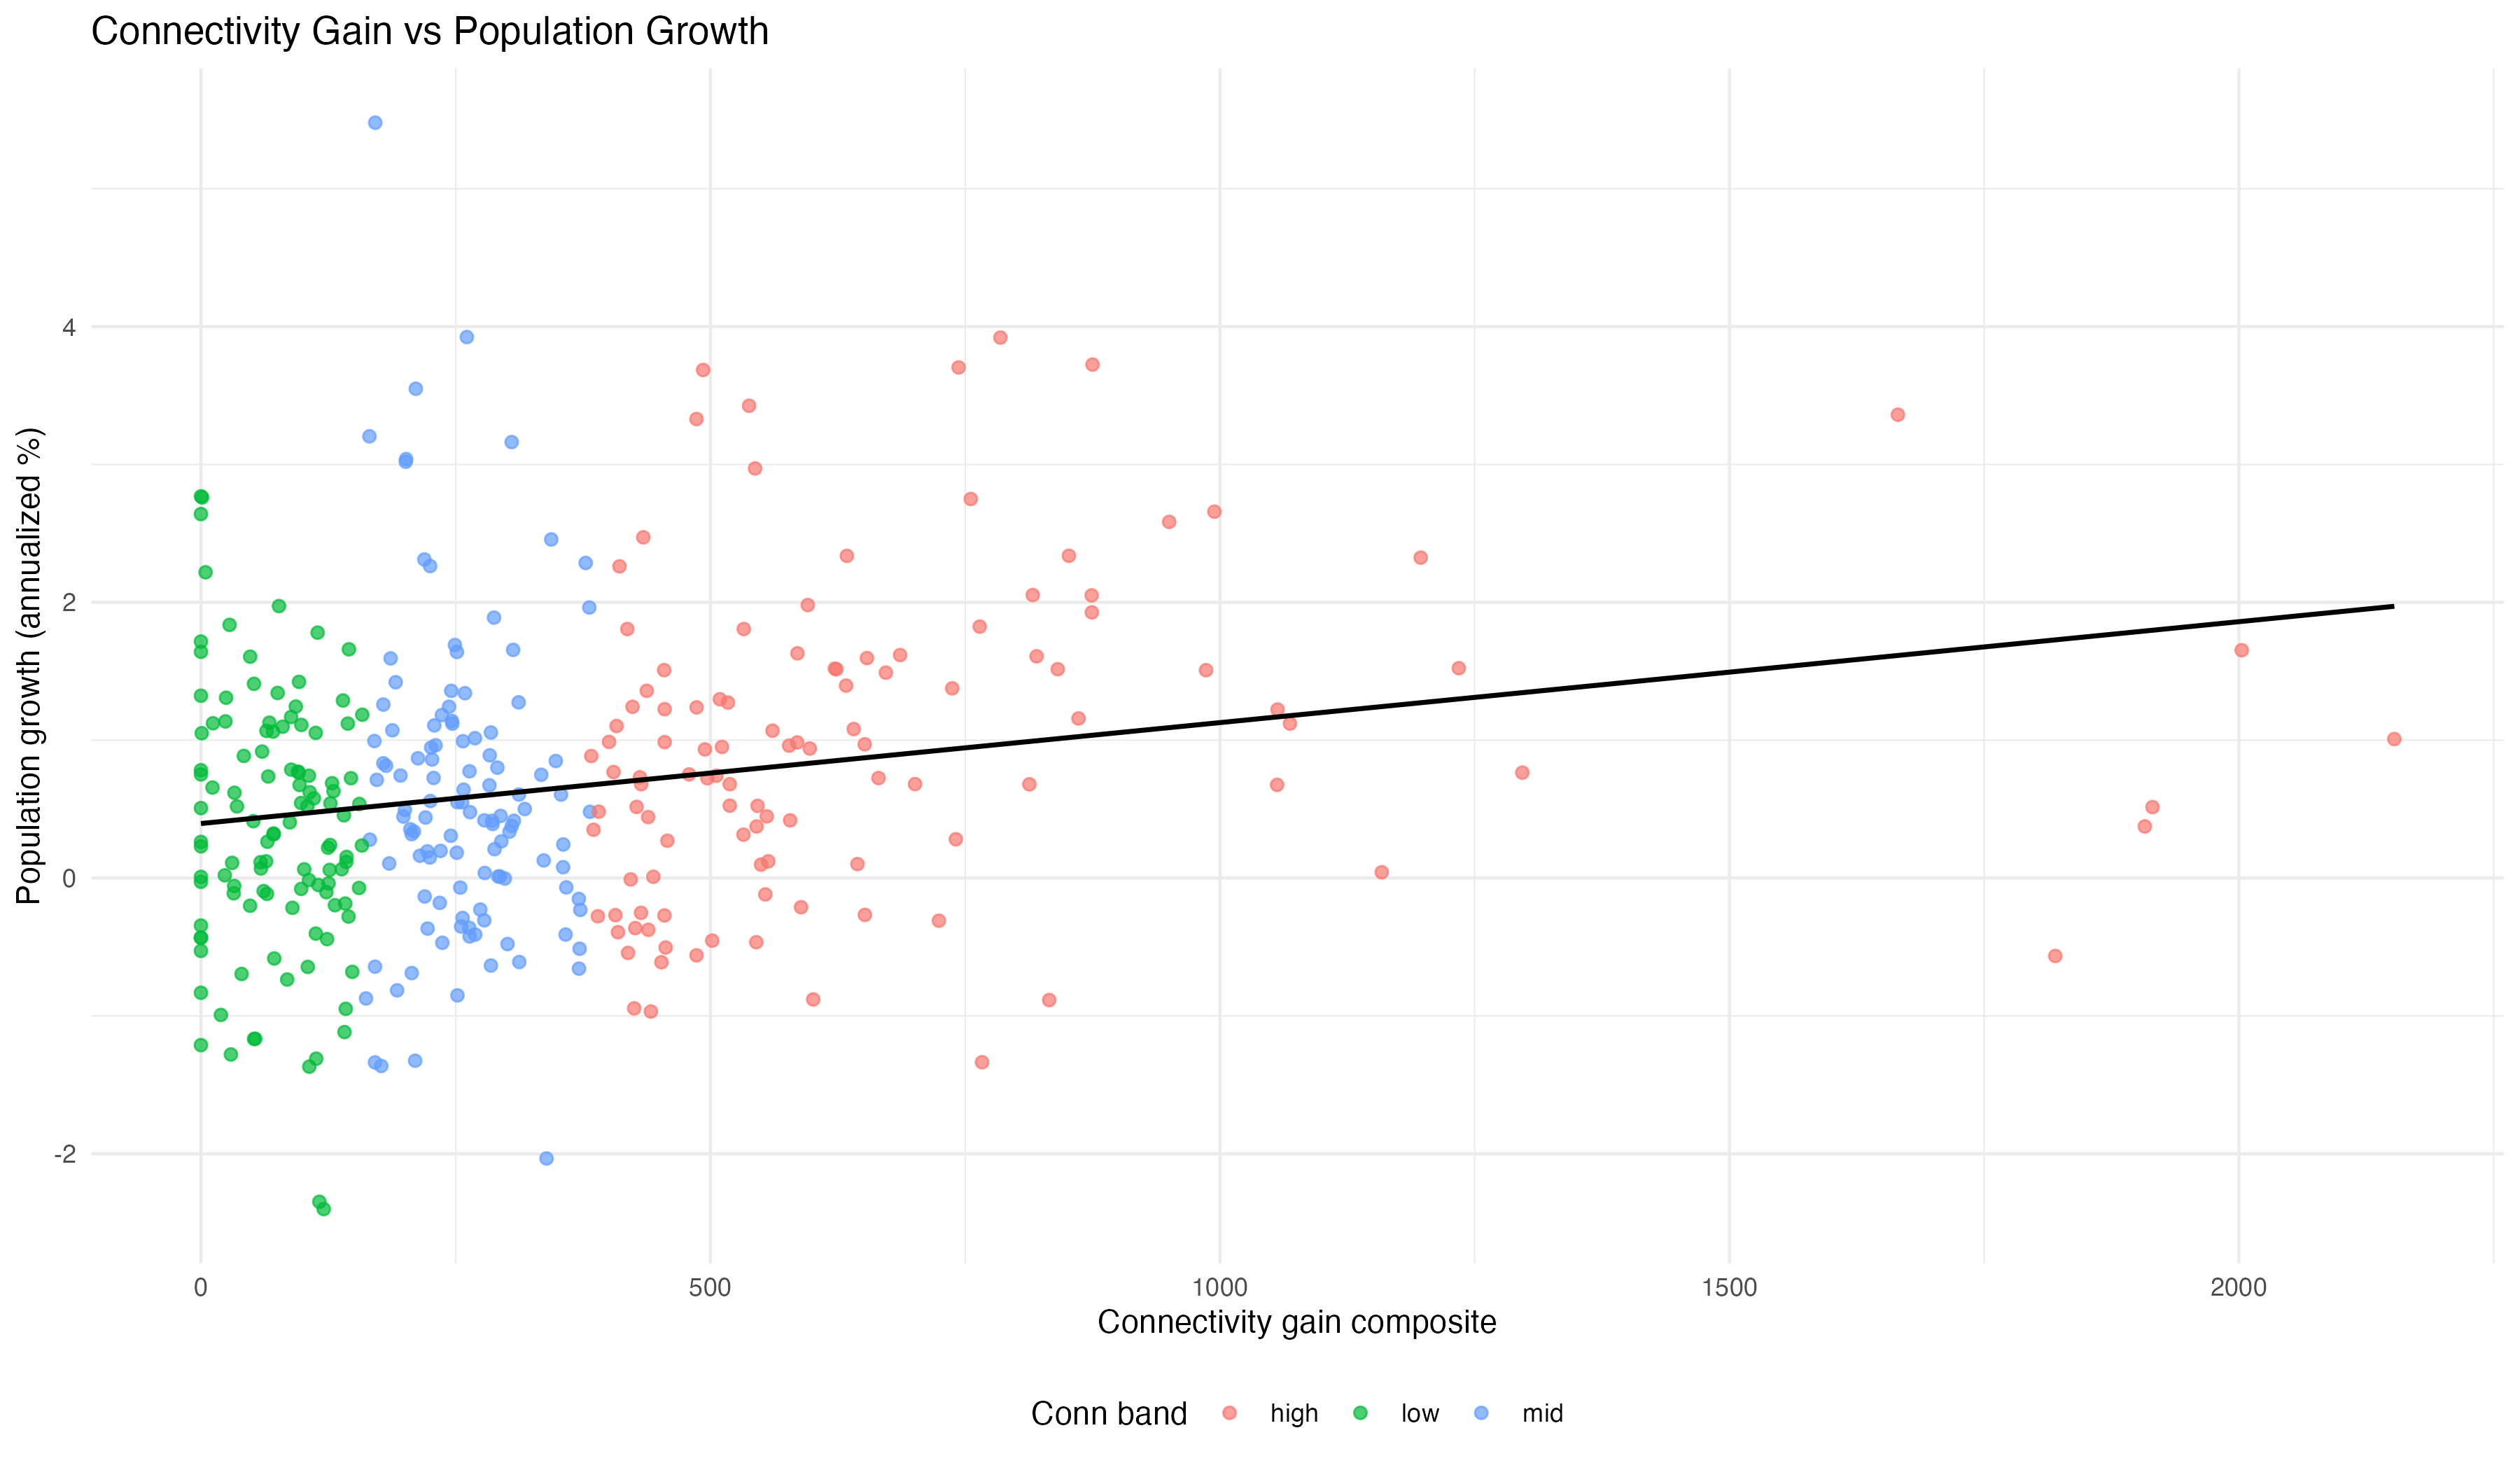
\includegraphics[width=\linewidth,height=0.72\textheight,keepaspectratio]{outputs/figures/fig_13_scatter_connectivity_vs_pop_growth.png}
\end{columns}
\small
The scatter evidence supports a broad positive coupling structure, but with considerable heterogeneity and nontrivial dispersion across trajectory classes.
\end{frame}

\begin{frame}{Policy-Transport Interaction Signal}
\small
\begin{columns}[T,onlytextwidth]
\column{0.53\linewidth}
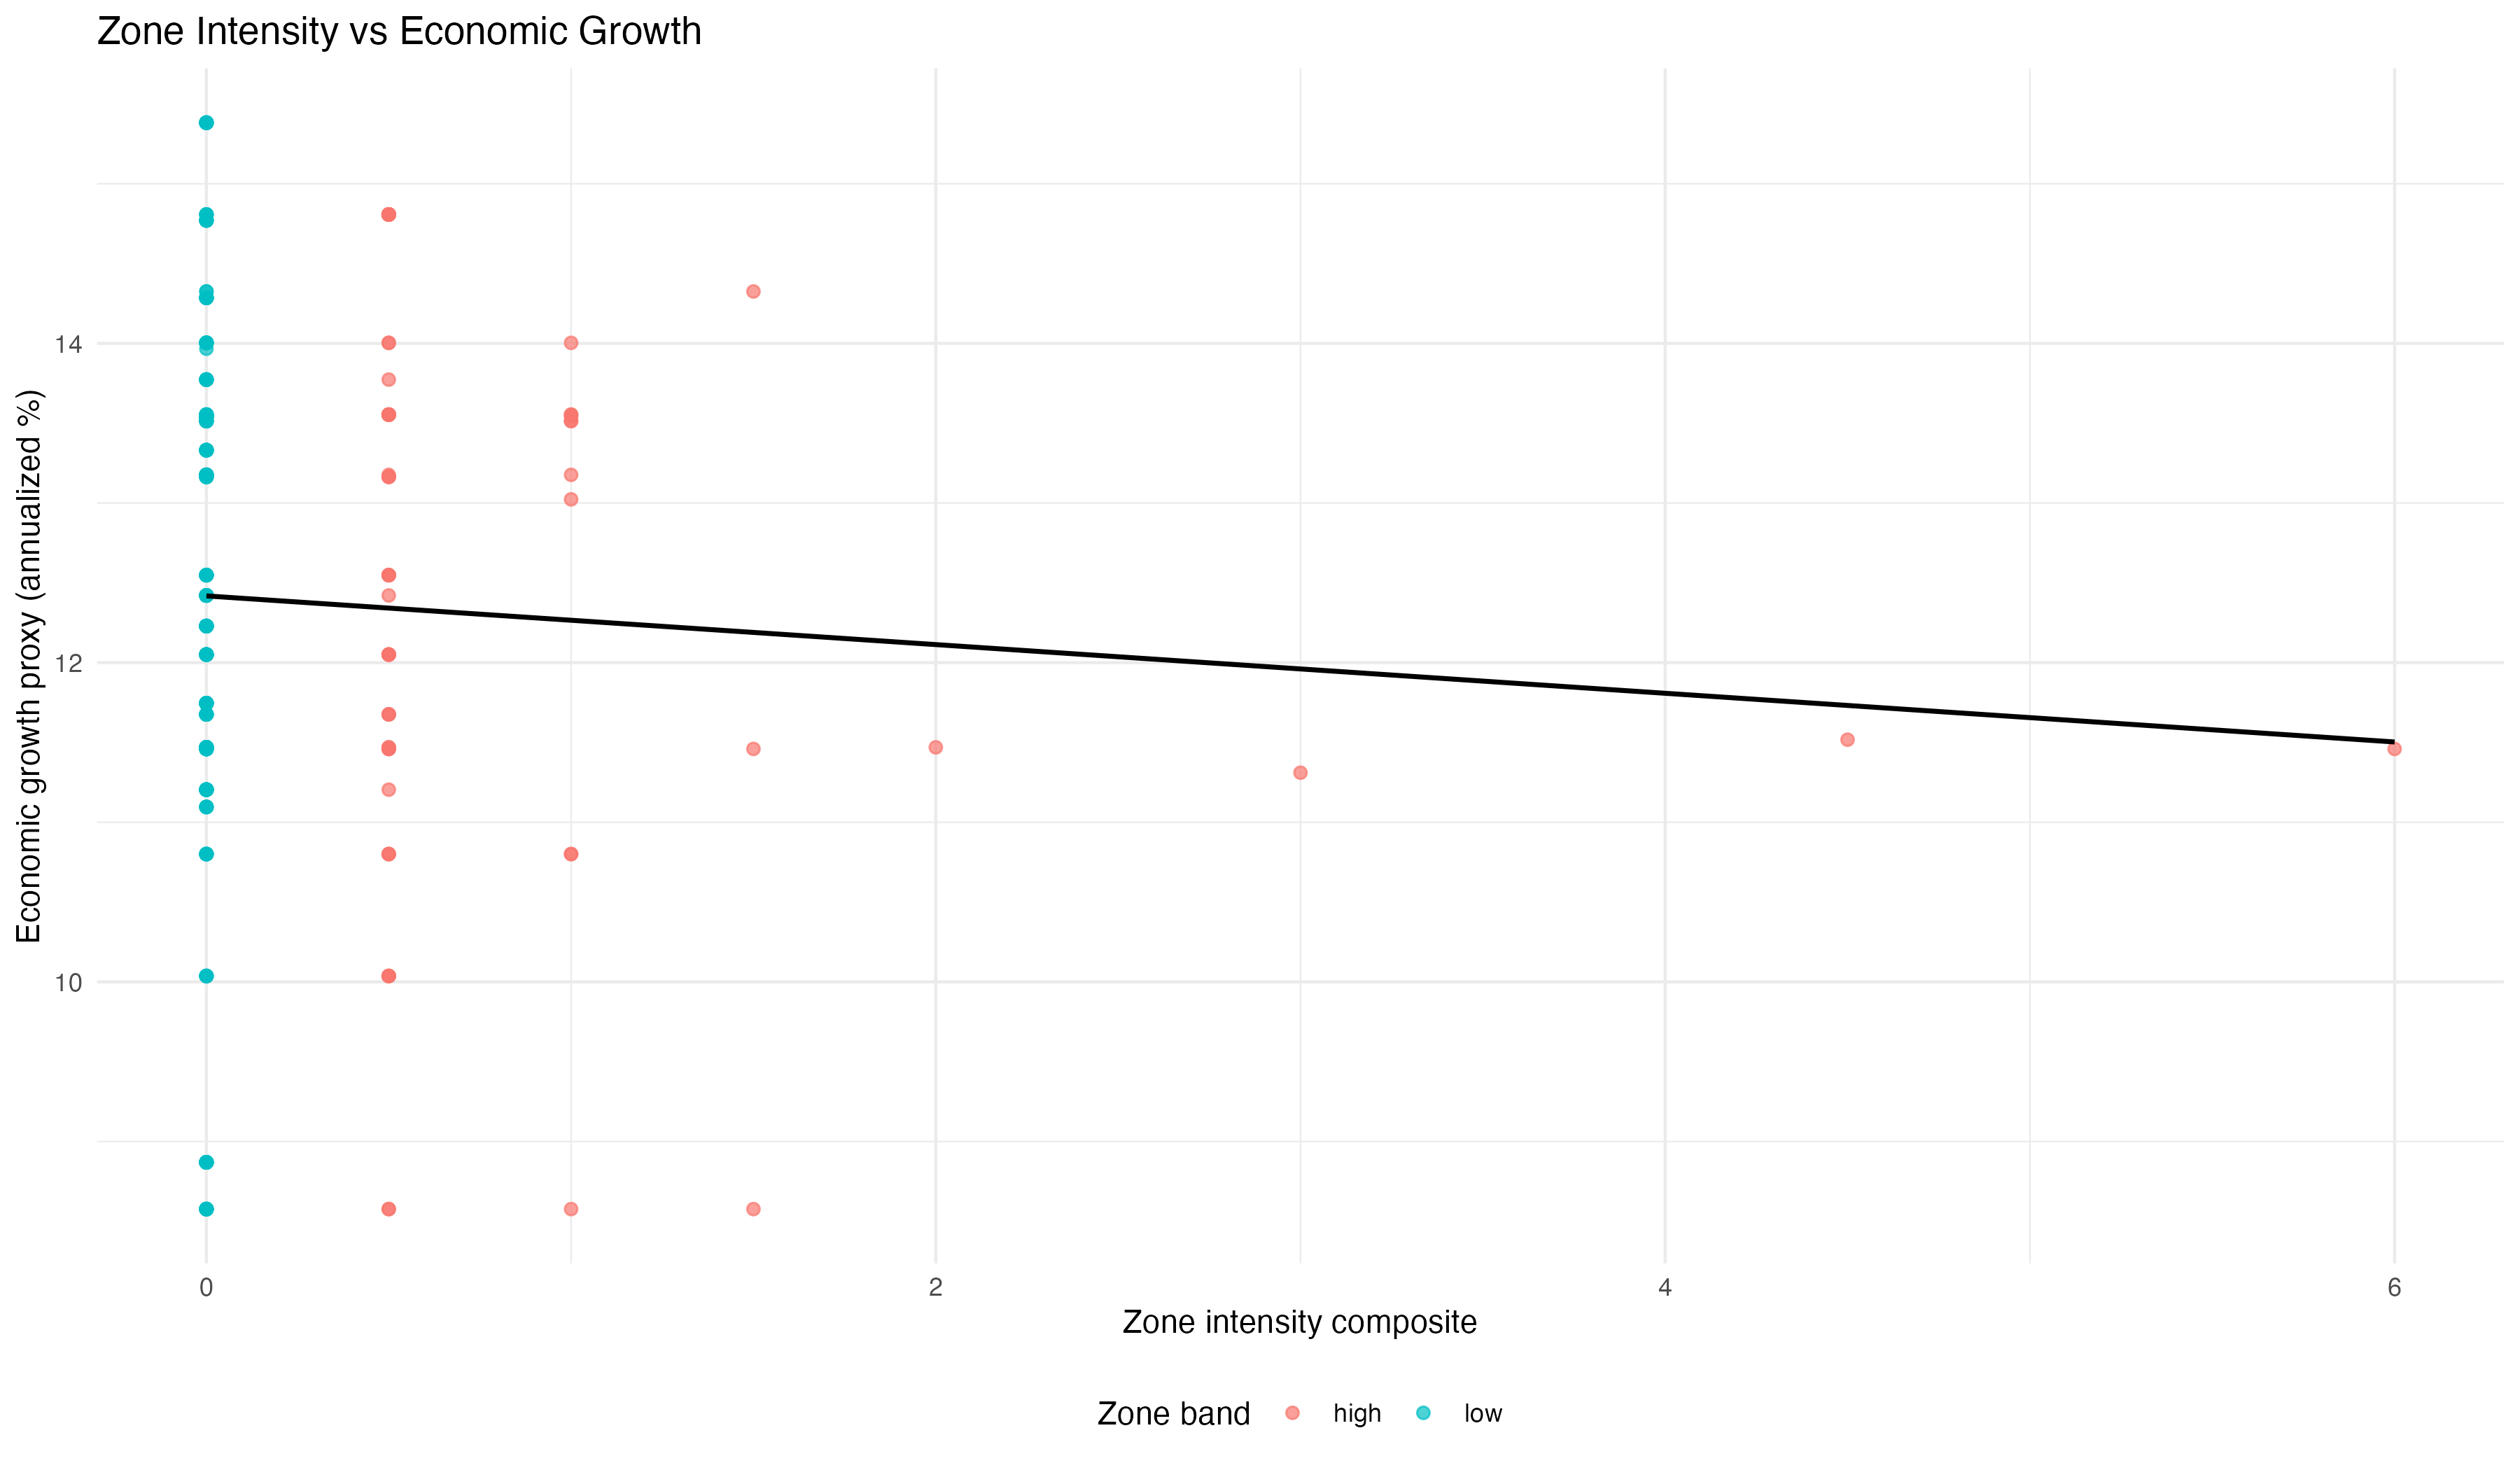
\includegraphics[width=\linewidth,height=0.72\textheight,keepaspectratio]{outputs/figures/fig_14_scatter_zone_vs_econ_growth.png}
\column{0.45\linewidth}
\justifying
\textbf{Interpretation:}
\begin{itemize}
  \item Zone intensity alone is not a universal guarantee of high growth.
  \item Stronger outcomes are more credible where zone intensity and connectivity gains co-occur.
  \item This supports a complementarity narrative over a single-factor narrative.
\end{itemize}
\end{columns}
\end{frame}

\begin{frame}{Typology Robustness Across Specifications}
\small
\begin{table}
\centering
\begin{tabular}{p{0.32\linewidth} p{0.16\linewidth} p{0.16\linewidth} p{0.14\linewidth}}
\toprule
Variant & Share Same as Baseline & ARI vs Baseline & Classes \\
\midrule
Baseline q33--q67 & 1.000 & 1.000 & 7 \\
Conn station heavy & 0.994 & 0.991 & 7 \\
Conn length heavy & 0.985 & 0.966 & 7 \\
Quantile q40--q60 & 0.869 & 0.694 & 7 \\
Quantile q25--q75 & 0.849 & 0.613 & 7 \\
\bottomrule
\end{tabular}
\end{table}
\smallskip
The class system is stable under substantial perturbations, especially weighting shifts.
\end{frame}

\begin{frame}{Key Quantitative Results (Executive Readout)}
\small
\begin{itemize}
  \item Population concentration change (HHI): \textbf{+11.84\%}.
  \item Economic concentration change (HHI): \textbf{+0.73\%}.
  \item HSR near-far population gap: \textbf{+0.019 pp/year}, CI crosses zero, p=0.921.
  \item HSR near-far economic gap: \textbf{+0.762 pp/year}, CI positive, p=0.011.
  \item Driver model coefficient (HSR km change $\rightarrow$ population growth): \textbf{+0.297}, 95\% CI [0.116, 0.458].
  \item Driver model coefficient (HSR km change $\rightarrow$ economic growth): \textbf{+0.110}, 95\% CI [-0.010, 0.241], borderline.
\end{itemize}
\vspace{0.3em}
This is a precise, mixed-strength evidence profile, not a one-direction universal effect.
\end{frame}

\begin{frame}{Interpretation: What the Study Supports}
\small
\begin{itemize}
  \item China's prefectural transformation is multi-regime and spatially uneven; a single national story is analytically misleading.
  \item Transport expansion, especially HSR accessibility, aligns more strongly with economic-growth differentials than with population-growth differentials in baseline corridor contrasts.
  \item Policy-zone intensity appears most informative when interpreted jointly with connectivity metrics and baseline conditions.
  \item Robustness scans show that some results are threshold-sensitive, which is exactly why uncertainty and sensitivity are now reported explicitly.
\end{itemize}
\end{frame}

\begin{frame}{Interpretation: What the Study Does \emph{Not} Claim}
\small
\begin{itemize}
  \item It does \textbf{not} claim causal treatment effects of HSR or zones.
  \item It does \textbf{not} claim prefecture GDP levels are official measurements; they are a disciplined proxy.
  \item It does \textbf{not} claim every near-HSR prefecture outperforms every far-HSR prefecture.
  \item It does \textbf{not} claim station access, line length, and zone intensity are independent drivers; they can co-move structurally.
\end{itemize}
\vspace{0.3em}
The analysis is strong descriptive evidence with explicit uncertainty boundaries.
\end{frame}

\begin{frame}{Policy Implications}
\small
\begin{itemize}
  \item Corridor policies should be targeted: benefits appear strongest in specific proximity bands (roughly 10--20 km in this setup).
  \item Transport investment alone is unlikely to maximize outcomes without complementary zone and local-development design.
  \item Regions in mixed or lagging typologies may need differentiated intervention bundles rather than uniform infrastructure-first programs.
  \item Monitoring frameworks should include uncertainty-aware diagnostics, not only headline mean-difference claims.
\end{itemize}
\end{frame}

\begin{frame}{Methodological Limitations and Next Upgrades}
\small
\textbf{Current limitations}
\begin{itemize}
  \item Development-zone inventory completeness is constrained by Wikidata point coverage.
  \item Economic activity uses a population-allocation proxy from provincial GDP.
  \item Population snapshots are periodic (GPW), not annual demographic accounting.
\end{itemize}
\textbf{Next technical upgrades}
\begin{itemize}
  \item Swap in official prefecture GDP series where available.
  \item Add additional controls for industrial structure and initial urbanization.
  \item Add spatial dependence diagnostics (e.g., Moran-type residual checks) and clustered uncertainty.
\end{itemize}
\end{frame}

\begin{frame}{Reproducibility and Output Suite}
\small
\begin{itemize}
  \item Pipeline script: \texttt{scripts/run\_china\_spatial\_reallocation.R}
  \item Core panel: \texttt{data/processed/analysis\_panel\_prefecture\_year.csv}
  \item Typology output: \texttt{data/processed/typology\_prefecture.csv}
  \item New robustness tables: \texttt{table\_hsr\_gap\_inference.csv}, \texttt{table\_hsr\_threshold\_sensitivity.csv}, \texttt{table\_driver\_regression\_bootstrap.csv}
  \item Narrative artifacts: \texttt{storyline\_evidence\_brief.md}, \texttt{method\_limitations\_reproducibility.md}
\end{itemize}
All artifacts are generated directly from the same deterministic pipeline.
\end{frame}

\begin{frame}{Final Takeaway}
\small
\begin{block}{One-sentence conclusion}
China's 2000--2020 prefectural transformation is heterogeneous, corridor-sensitive, and best explained by \emph{joint} transport-policy dynamics under explicit uncertainty, not by a single universal growth mechanism.
\end{block}
\vspace{0.4em}
\begin{itemize}
  \item The narrative is now sharper because it is tied to quantified uncertainty and robustness.
  \item The analysis is more comprehensive because multimodal, policy, demographic, and economic layers are integrated.
  \item The interpretation is methodologically tighter because over-claiming pathways are explicitly blocked.
\end{itemize}
\vfill
\centering
\textbf{Thank you.}
\end{frame}

\end{document}
